\documentclass[11pt,a4paper]{article}
\usepackage[a4paper,margin=21mm,headheight=15pt]{geometry}
\usepackage[T1]{fontenc}
\usepackage[utf8]{inputenc}
\usepackage{lmodern}
\usepackage{microtype}
\usepackage{graphicx}
\usepackage{float}
\usepackage{booktabs}
\usepackage{longtable}
\usepackage{array}
\usepackage{xcolor}
\usepackage{amsmath}
\usepackage{amssymb}
\usepackage{listings}
\usepackage{subcaption}
\usepackage{enumitem}
\usepackage{fancyhdr}
\usepackage[hidelinks]{hyperref}
\usepackage[most]{tcolorbox}
\usepackage{placeins}
\usepackage{titlesec}
\usepackage{lastpage}

\graphicspath{{figures/}}
\setlength{\parindent}{0pt}
\setlength{\parskip}{0.6em}
\renewcommand{\arraystretch}{1.14}
\setlist{itemsep=0.22em,topsep=0.3em}

\definecolor{navy}{HTML}{17324D}
\definecolor{teal}{HTML}{155E75}
\definecolor{softblue}{HTML}{EAF3F7}
\definecolor{softamber}{HTML}{FFF7E6}
\definecolor{softgrey}{HTML}{F3F4F6}
\definecolor{softgreen}{HTML}{EAF6EE}
\definecolor{softrose}{HTML}{FCEEEF}
\definecolor{codegreen}{HTML}{166534}

\hypersetup{pdftitle={Communication Engineering Laboratory Logbook -- Labs 1 to 5},pdfauthor={Aaron Taylor},colorlinks=true,linkcolor=navy,urlcolor=teal}
\pagestyle{fancy}
\fancyhf{}
\lhead{ENEL700 Communication Engineering}
\rhead{Laboratory Logbook}
\cfoot{\thepage\ of \pageref{LastPage}}
\titleformat{\section}{\Huge\bfseries\color{navy}}{}{0pt}{}
\titleformat{\subsection}{\Large\bfseries\color{teal}}{}{0pt}{}

\newtcolorbox{answerbox}{breakable,colback=softblue,colframe=teal,boxrule=0.7pt,arc=2mm,title=My answer,fonttitle=\bfseries}
\newtcolorbox{evidencebox}{breakable,colback=softgrey,colframe=navy,boxrule=0.6pt,arc=2mm,title=Evidence and what it supports,fonttitle=\bfseries}
\newtcolorbox{observationbox}{breakable,colback=softgreen,colframe=green!45!black,boxrule=0.6pt,arc=2mm,title=What I observed,fonttitle=\bfseries}
\newtcolorbox{checkbox}{breakable,colback=softamber,colframe=orange!65!black,boxrule=0.6pt,arc=2mm,title=*** Check or complete,fonttitle=\bfseries}
\newtcolorbox{notebox}{breakable,colback=softrose,colframe=red!55!black,boxrule=0.6pt,arc=2mm,title=Weekly lab note,fonttitle=\bfseries}
\newtcolorbox{placeholderbox}{breakable,colback=white,colframe=navy!45,boxrule=0.6pt,arc=2mm,title=Space retained for this lab,fonttitle=\bfseries}

\lstdefinestyle{matlab}{language=Matlab,basicstyle=\ttfamily\small,keywordstyle=\color{blue!65!black}\bfseries,commentstyle=\color{codegreen},stringstyle=\color{red!60!black},numbers=left,numberstyle=\tiny\color{gray},numbersep=8pt,frame=single,rulecolor=\color{gray!40},breaklines=true,showstringspaces=false,backgroundcolor=\color{gray!4}}

\newcommand{\weeklynote}[1]{\begin{notebox}#1\end{notebox}}
\newcommand{\labdivider}{\FloatBarrier\clearpage}

\begin{document}
\begin{titlepage}
\pagecolor{navy}\color{white}
\vspace*{25mm}
{\Huge\bfseries Communication Engineering\\[0.25em]Laboratory Logbook\par}
\vspace{8mm}
{\Large Labs 1--5: practical work, evidence and answered questions\par}
\vfill
\begin{tcolorbox}[colback=white,colframe=white,coltext=navy,boxrule=0.7pt,arc=3mm]
\Large\textbf{Student:} Aaron Taylor\\[0.4em]
\textbf{Course:} ENEL700 Communication Engineering\\[0.4em]
\textbf{Academic year:} 2026\\[0.4em]
\textbf{Group:} *** confirm names for the title page
\end{tcolorbox}
\vfill
{\large A working document. Unsupported details are marked with *** rather than guessed.\par}
\end{titlepage}
\nopagecolor\color{black}

\begin{evidencebox}
This is a practical logbook rather than a formal laboratory report. Each laboratory has its own section for what I did, what I should examine, answers to the manual questions, important evidence, and the short weekly note written after the session. The original photographs and class files remain the primary evidence. Duplicate photographs are not repeated merely to make the document look fuller.
\end{evidencebox}
\tableofcontents
\clearpage
\section{Lab 1 -- Amplitude Modulation}
\begin{placeholderbox}
This section is deliberately retained for Lab 1 material. No technical content has been inserted yet because I have not supplied the class evidence or weekly note.
\vspace{30mm}
\end{placeholderbox}
\subsection{Questions or points to examine}
\begin{checkbox}*** Add the Lab 1 manual questions, observations and evidence when they are available.\end{checkbox}
\weeklynote{\textbf{Date:} ***\\\textbf{Who attended / roles:} ***\\\textbf{What we achieved:} ***\\\textbf{What was difficult:} ***\\\textbf{What I will do differently next time:} ***\vspace{18mm}}
\labdivider

\section{Lab 2 -- Frequency Modulation}
\begin{placeholderbox}
This section is deliberately retained for Lab 2 material. No technical content has been inserted yet because I have not supplied the class evidence or weekly note.
\vspace{30mm}
\end{placeholderbox}
\subsection{Questions or points to examine}
\begin{checkbox}*** Add the Lab 2 manual questions, observations and evidence when they are available.\end{checkbox}
\weeklynote{\textbf{Date:} ***\\\textbf{Who attended / roles:} ***\\\textbf{What we achieved:} ***\\\textbf{What was difficult:} ***\\\textbf{What I will do differently next time:} ***\vspace{18mm}}
\labdivider
\section{Lab 3 -- Binary Phase-Shift Keying}
\subsection{Purpose and practical arrangement}
The objective was to use the TIMS equipment to investigate a digitally modulated binary phase-shift keying signal. I generated BPSK by multiplying a sinusoidal carrier by a bipolar NRZ-L sequence. A change in data polarity reverses the carrier polarity, which is equivalent to a $180^\circ$ phase change. The manual arranged the carrier at four times the bit-clock rate, used a tuneable low-pass filter to investigate transmitter bandwidth, and used a stolen synchronous carrier for demodulation.

\begin{checkbox}
\textbf{Session details still needed:} *** confirm the Lab 3 date, who attended, how the work was divided, and the short personal note you want at the bottom of this section. One oscilloscope display visibly shows 13-Aug-26, but I have not treated that instrument date as proof of the full attendance record.
\end{checkbox}

\begin{figure}[H]\centering
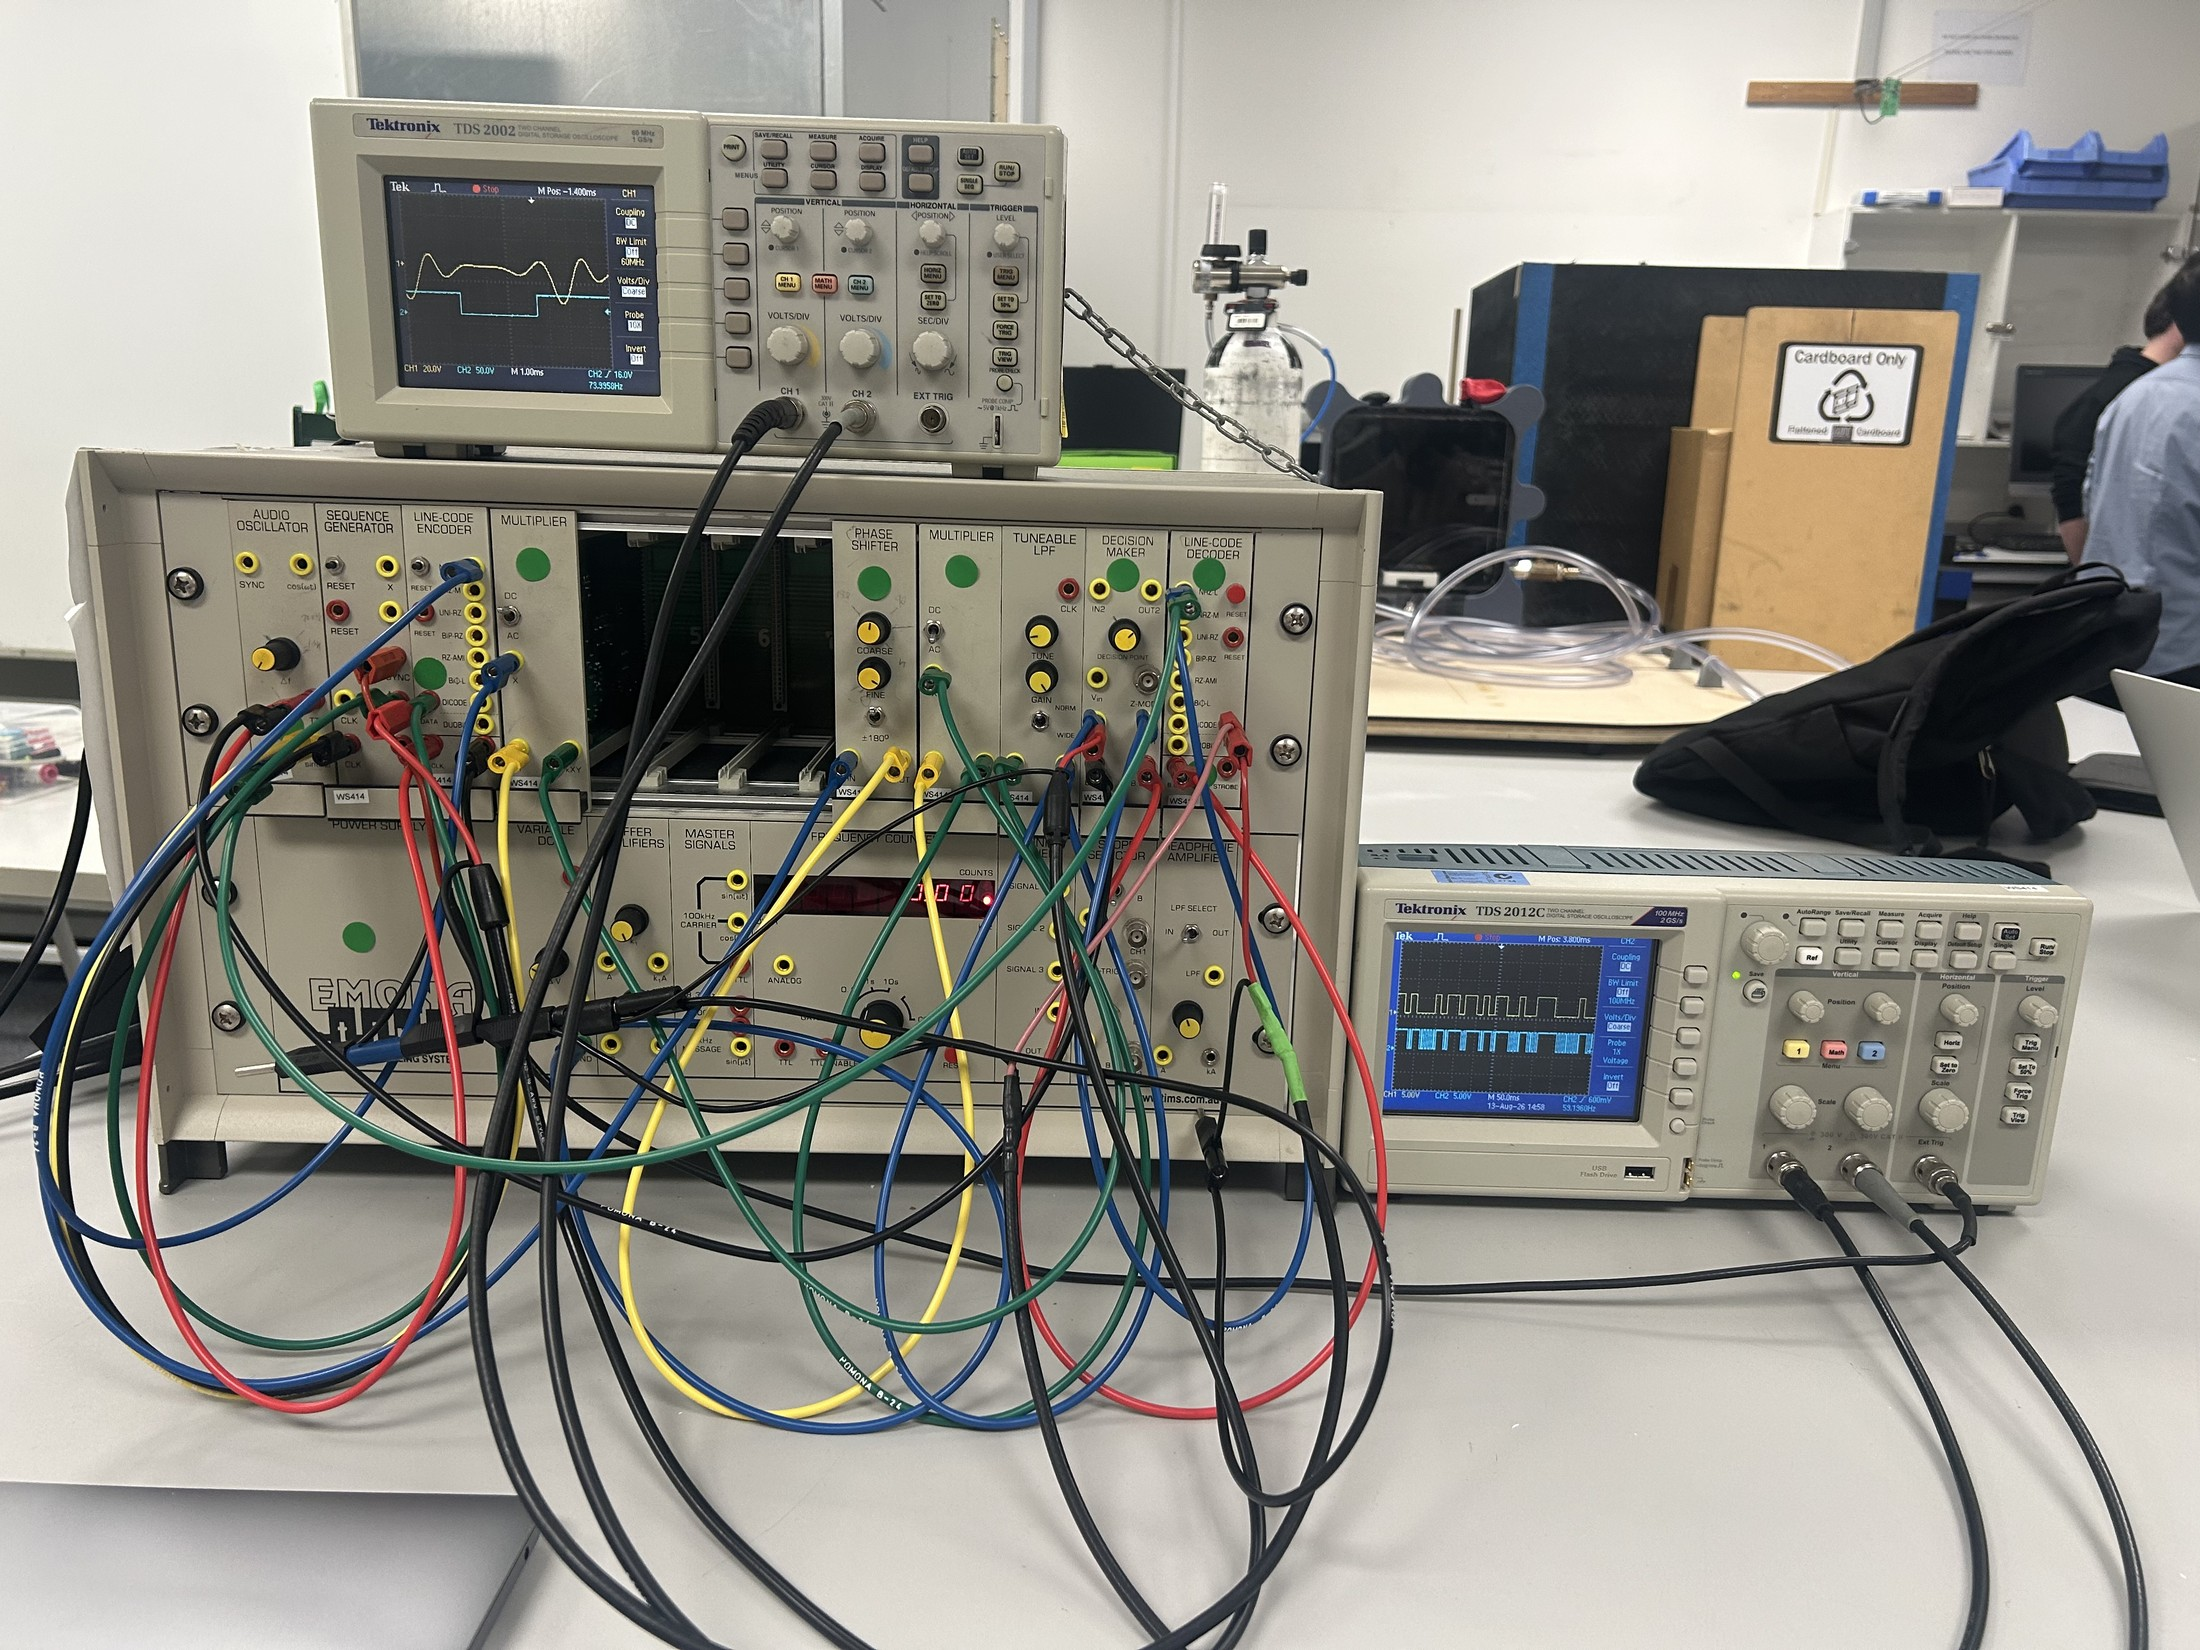
\includegraphics[width=0.98\textwidth]{lab3_full_setup.jpg}
\caption{Primary physical evidence for Lab 3. The TIMS patch includes the AUDIO OSCILLATOR, SEQUENCE GENERATOR, LINE-CODE ENCODER, MULTIPLIER, PHASE SHIFTER, second MULTIPLIER, TUNEABLE LPF, DECISION MAKER and LINE-CODE DECODER. Two oscilloscopes were used to view analogue/modulated and digital-related signals.}
\label{fig:lab3-setup}\end{figure}

\subsection{What the manual asked me to investigate}
\begin{enumerate}
\item Patch the Figure 10 BPSK generator; inspect carrier phase reversals as the bit-clock/carrier phase is changed; vary transmitter low-pass-filter bandwidth and observe the envelope.
\item Patch the Figure 11 synchronous demodulator; compare the tuneable-LPF output with the transmitted sequence and correct an inverted result with the receiver's $180^\circ$ phase switch.
\item Configure the DECISION MAKER for NRZ-L, set its input near the TIMS analogue reference level, adjust the decision point and inspect the regenerated output.
\item Observe the LINE-CODE DECODER TTL output and check whether recovered polarity still depends on receiver carrier phase.
\item Change transmitter bandwidth and inspect the resulting amplitude at the DECISION MAKER input.
\end{enumerate}

\subsection{Observed BPSK and transition behaviour}
\begin{figure}[H]\centering
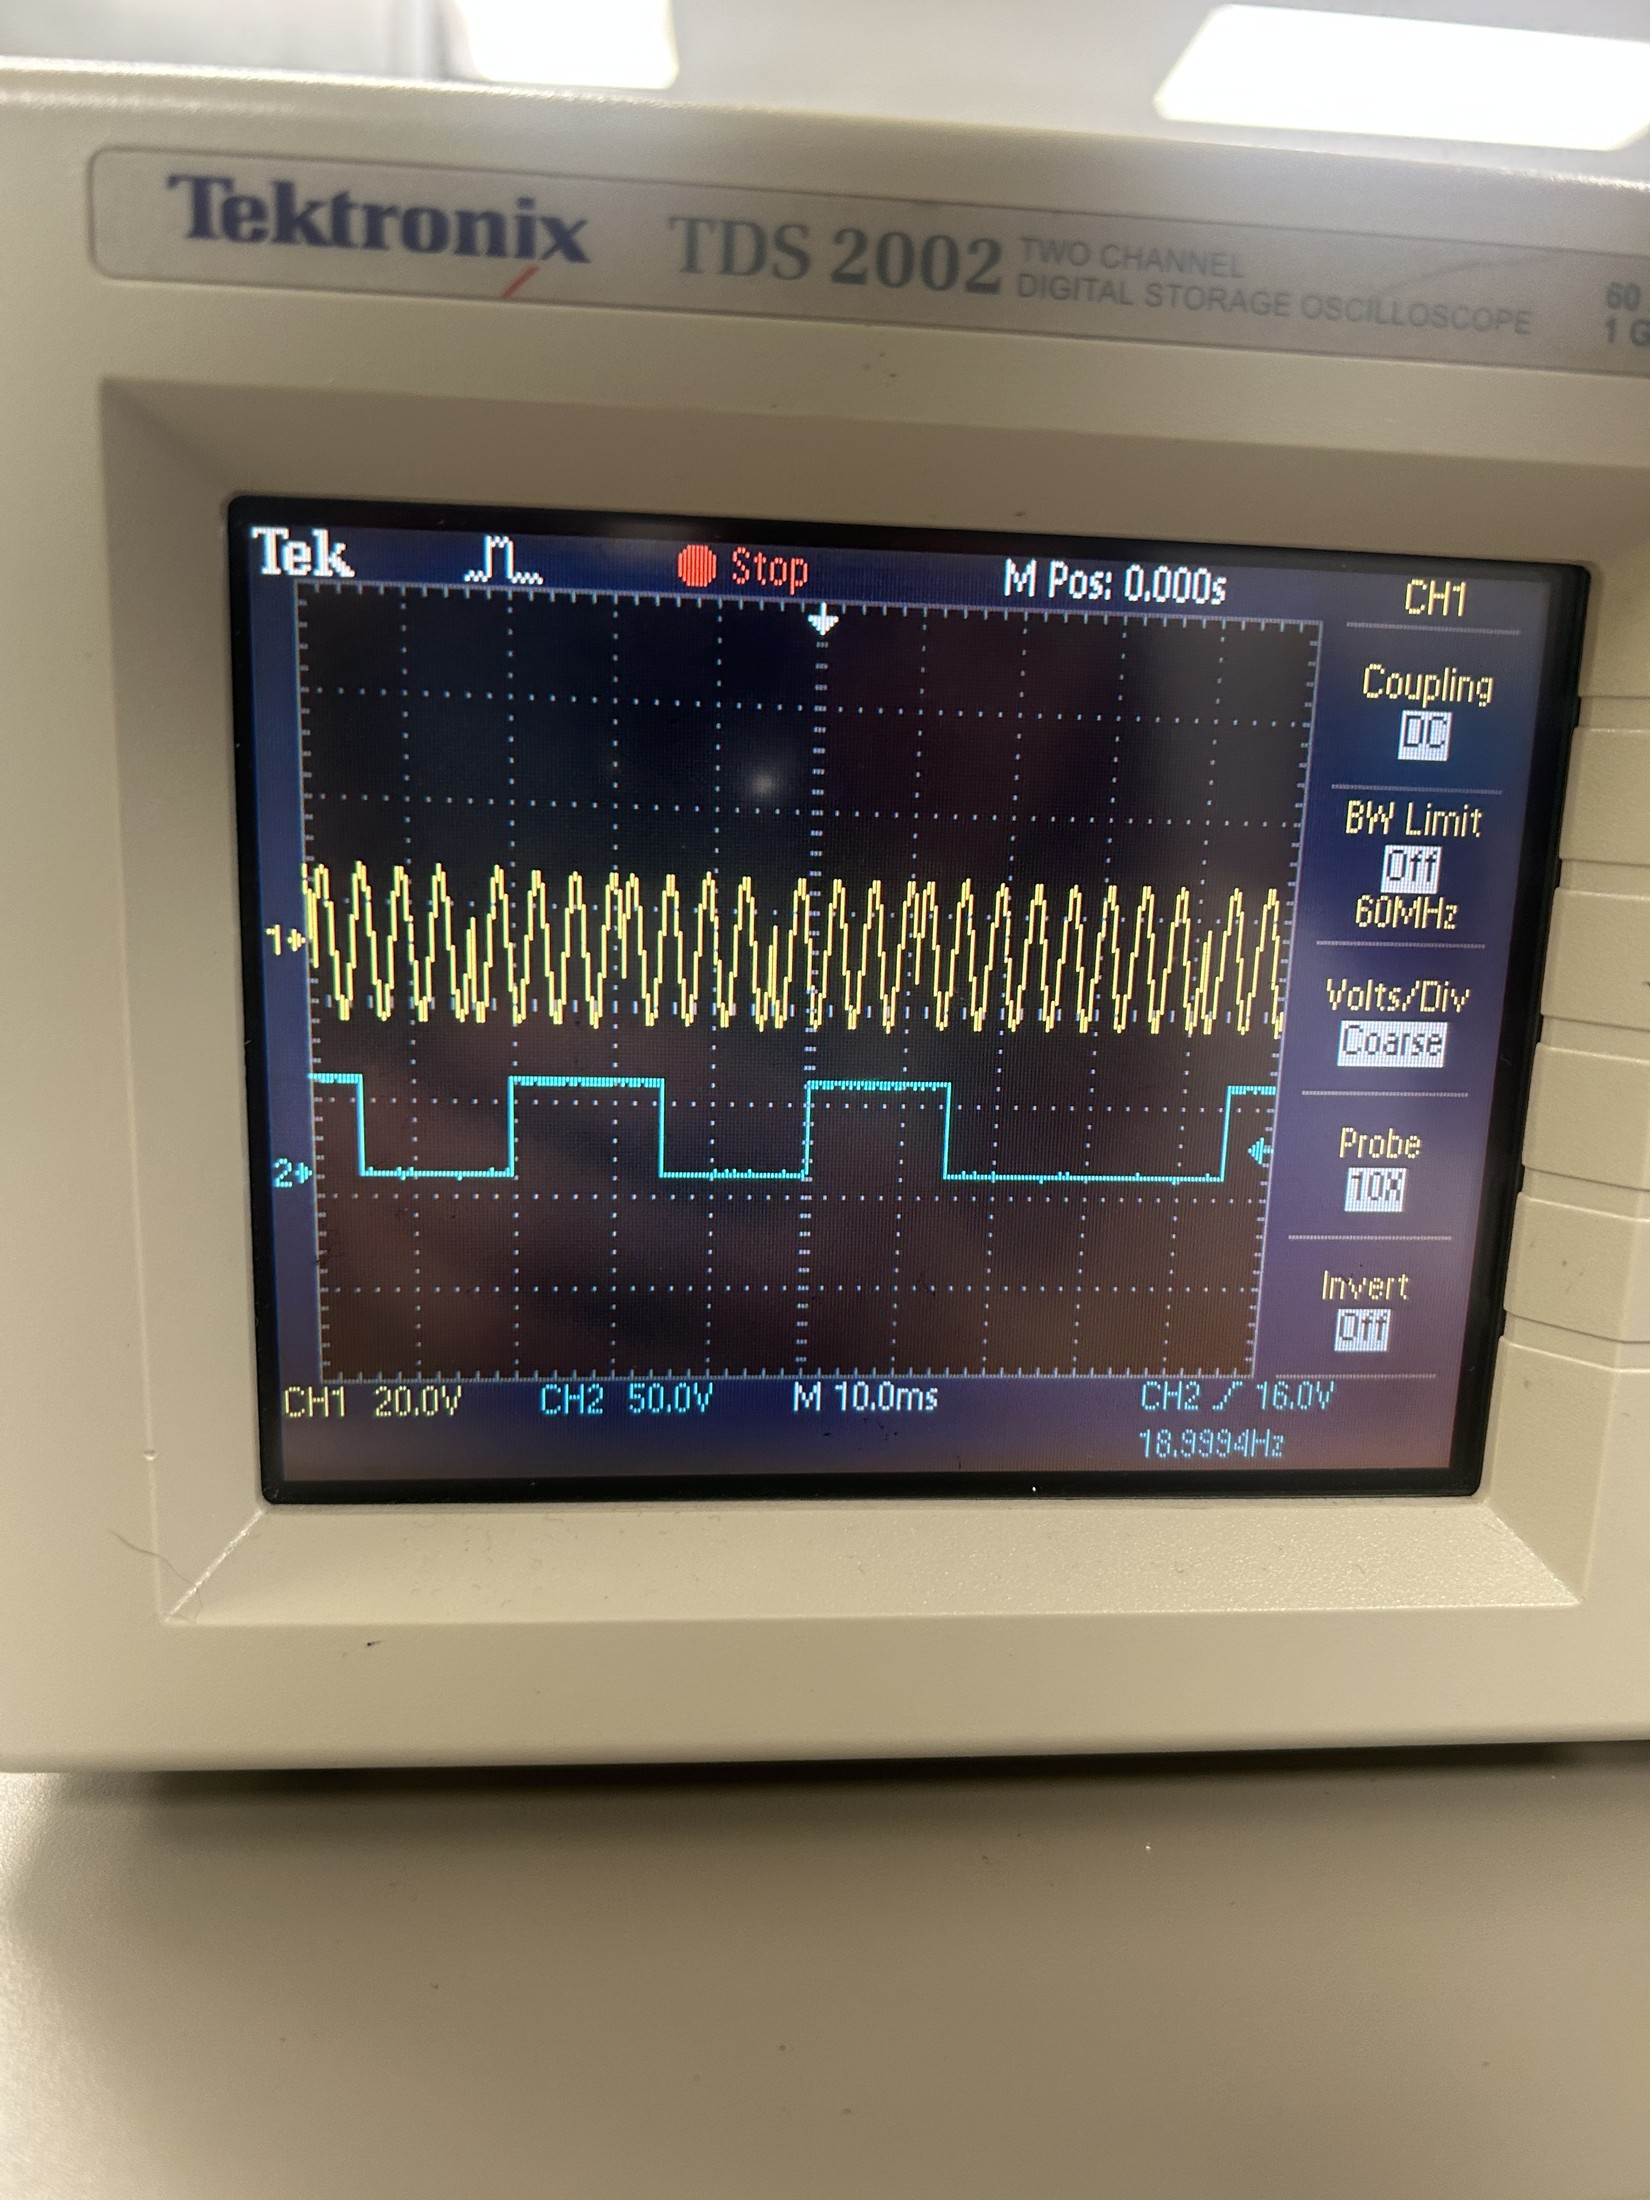
\includegraphics[width=0.63\textwidth]{lab3_bpsk_phase_transitions.jpg}
\caption{A clear class capture of a high-frequency yellow waveform viewed against a cyan binary sequence. The display shows CH1 20.0 V/div, CH2 50.0 V/div, 10.0 ms/div and a visible frequency readout of about 18.99 Hz for the selected channel. The repeated carrier-like waveform changes its relationship to the data at the sequence transitions, supporting the BPSK phase-transition investigation.}
\label{fig:lab3-bpsk}\end{figure}

\begin{observationbox}
The carrier-like waveform remained present through both data states, but its polarity/phase relationship changed at data transitions. This is the central visible feature of BPSK: the information is conveyed by phase choice rather than by simply turning the carrier off. Because the carrier and bit clock were harmonically related, the transitions appeared in repeatable positions relative to the bit sequence.
\end{observationbox}

\subsection{Bandwidth and demodulated waveform shape}
\begin{figure}[H]\centering
\begin{subfigure}[t]{0.49\textwidth}\centering
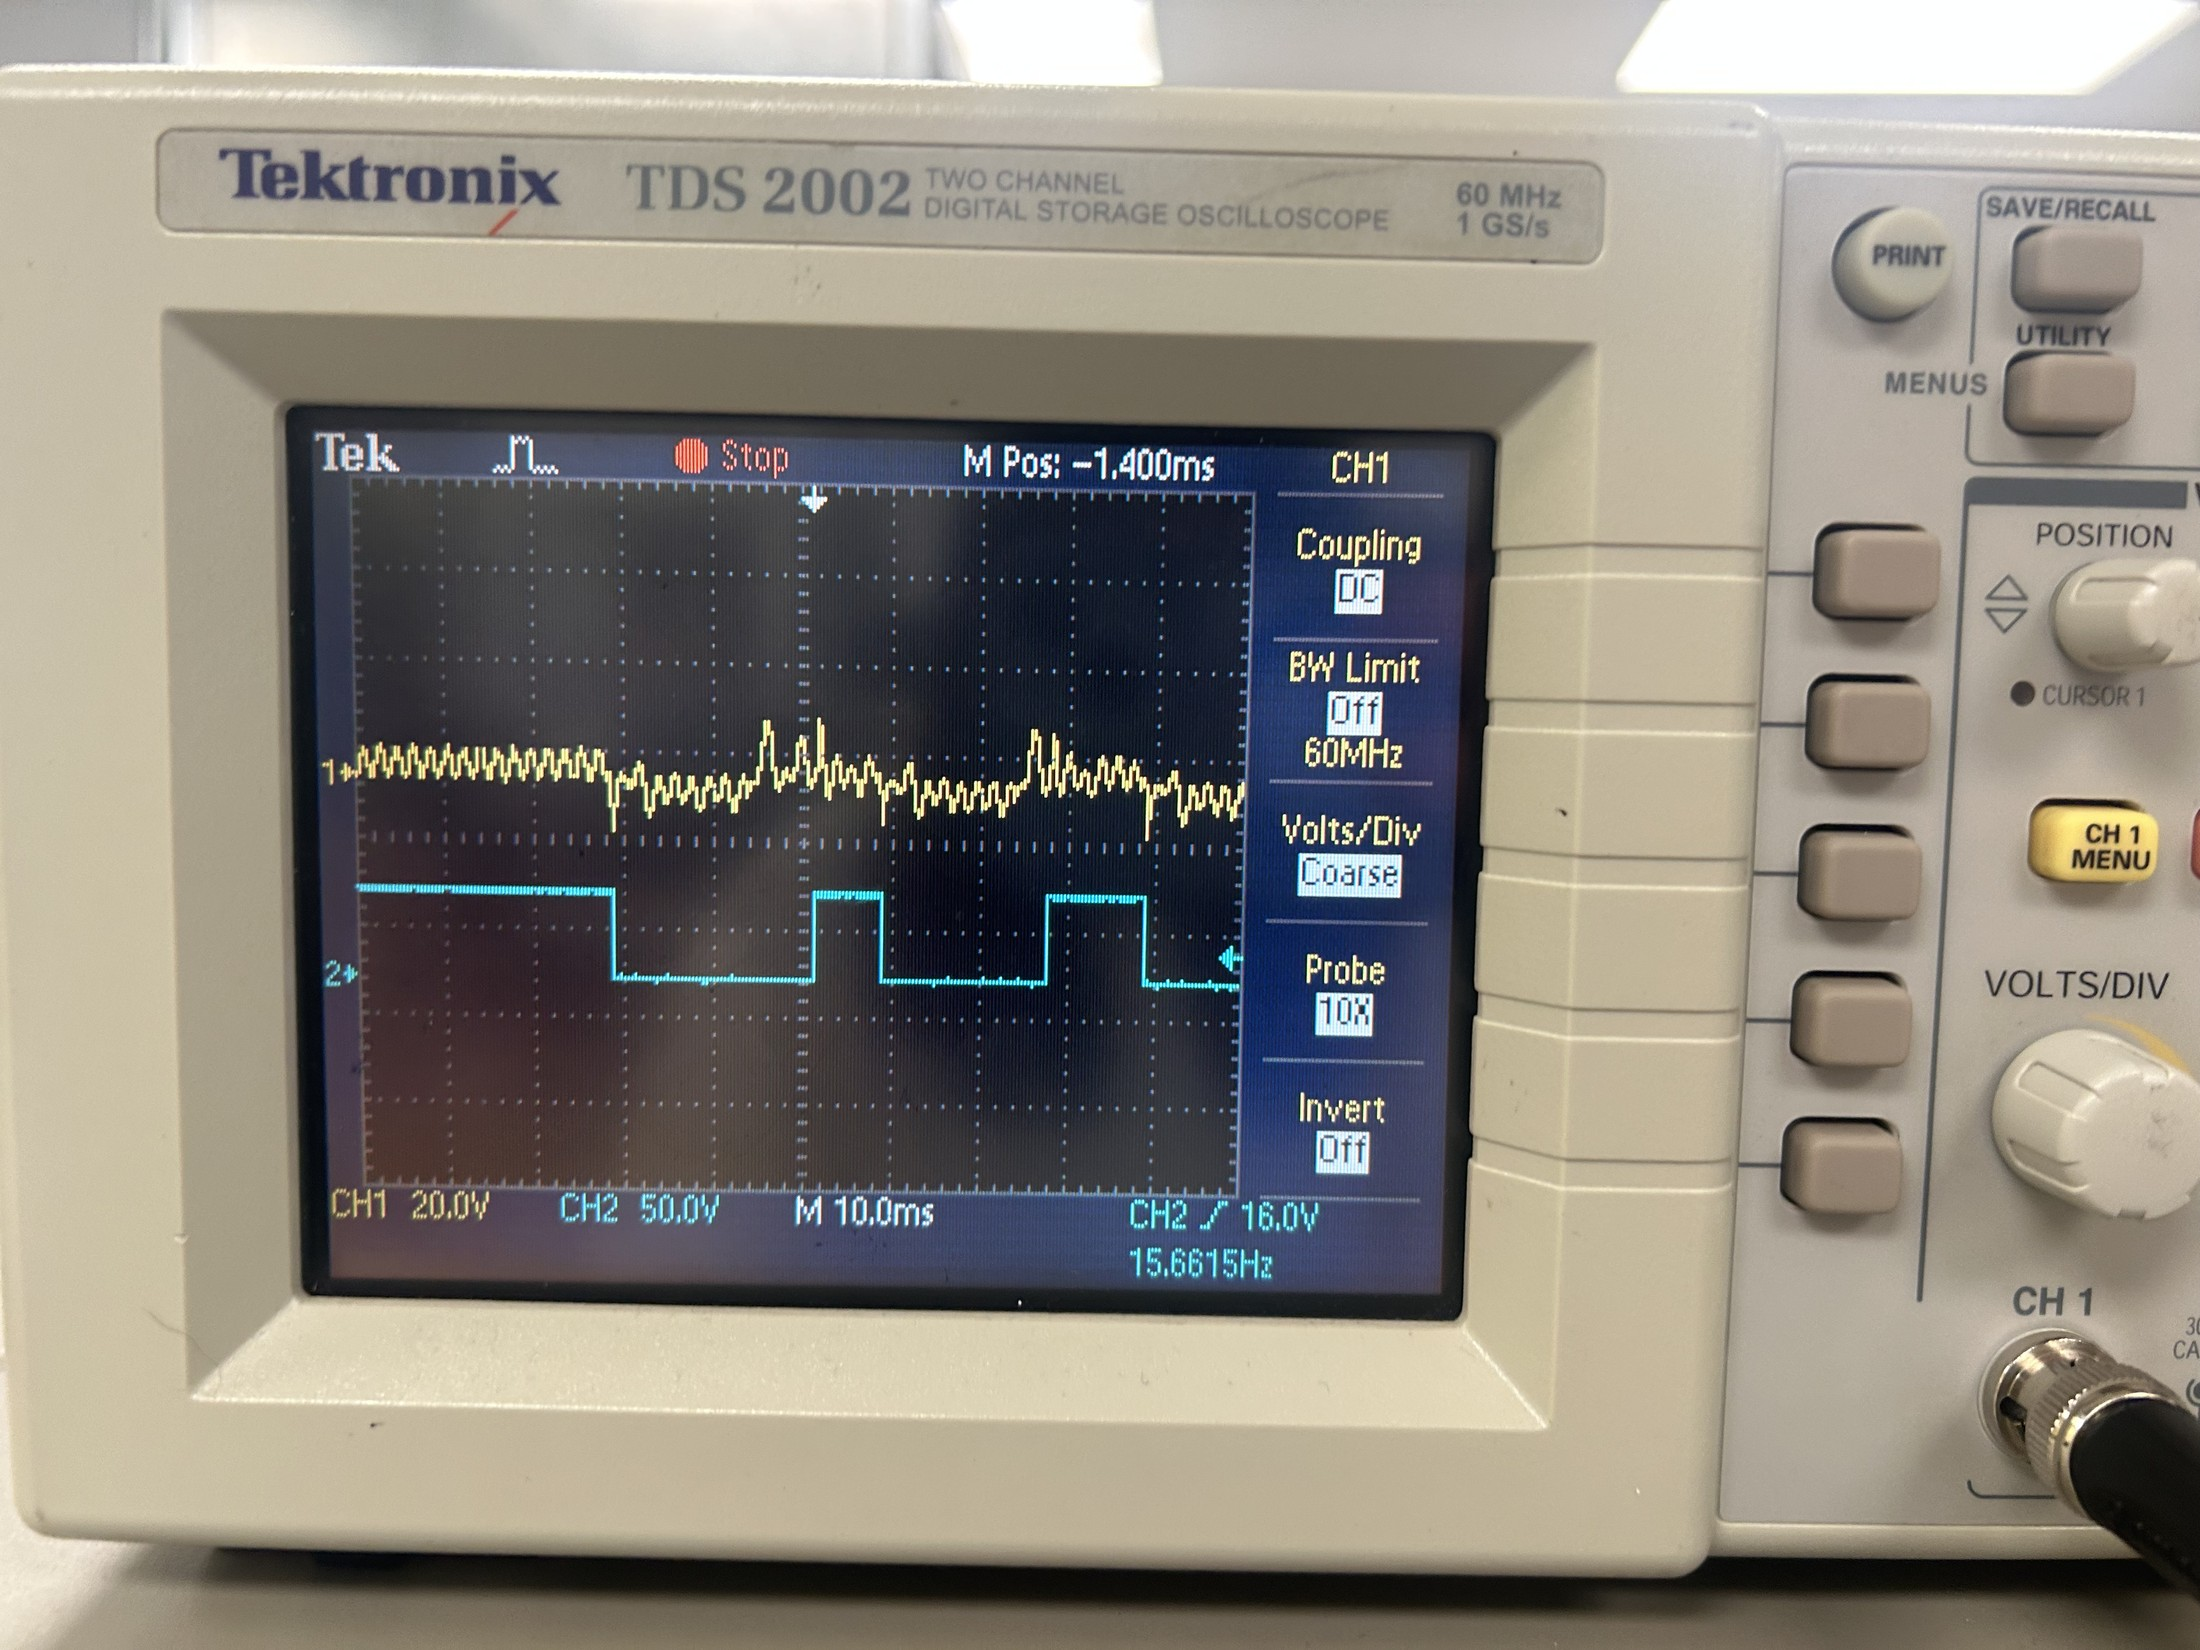
\includegraphics[width=\linewidth]{lab3_bandlimited_transition.jpg}
\caption{Band-limited/noisy transition waveform compared with the binary sequence; 10.0 ms/div and about 15.66 Hz visible.}
\end{subfigure}\hfill
\begin{subfigure}[t]{0.49\textwidth}\centering
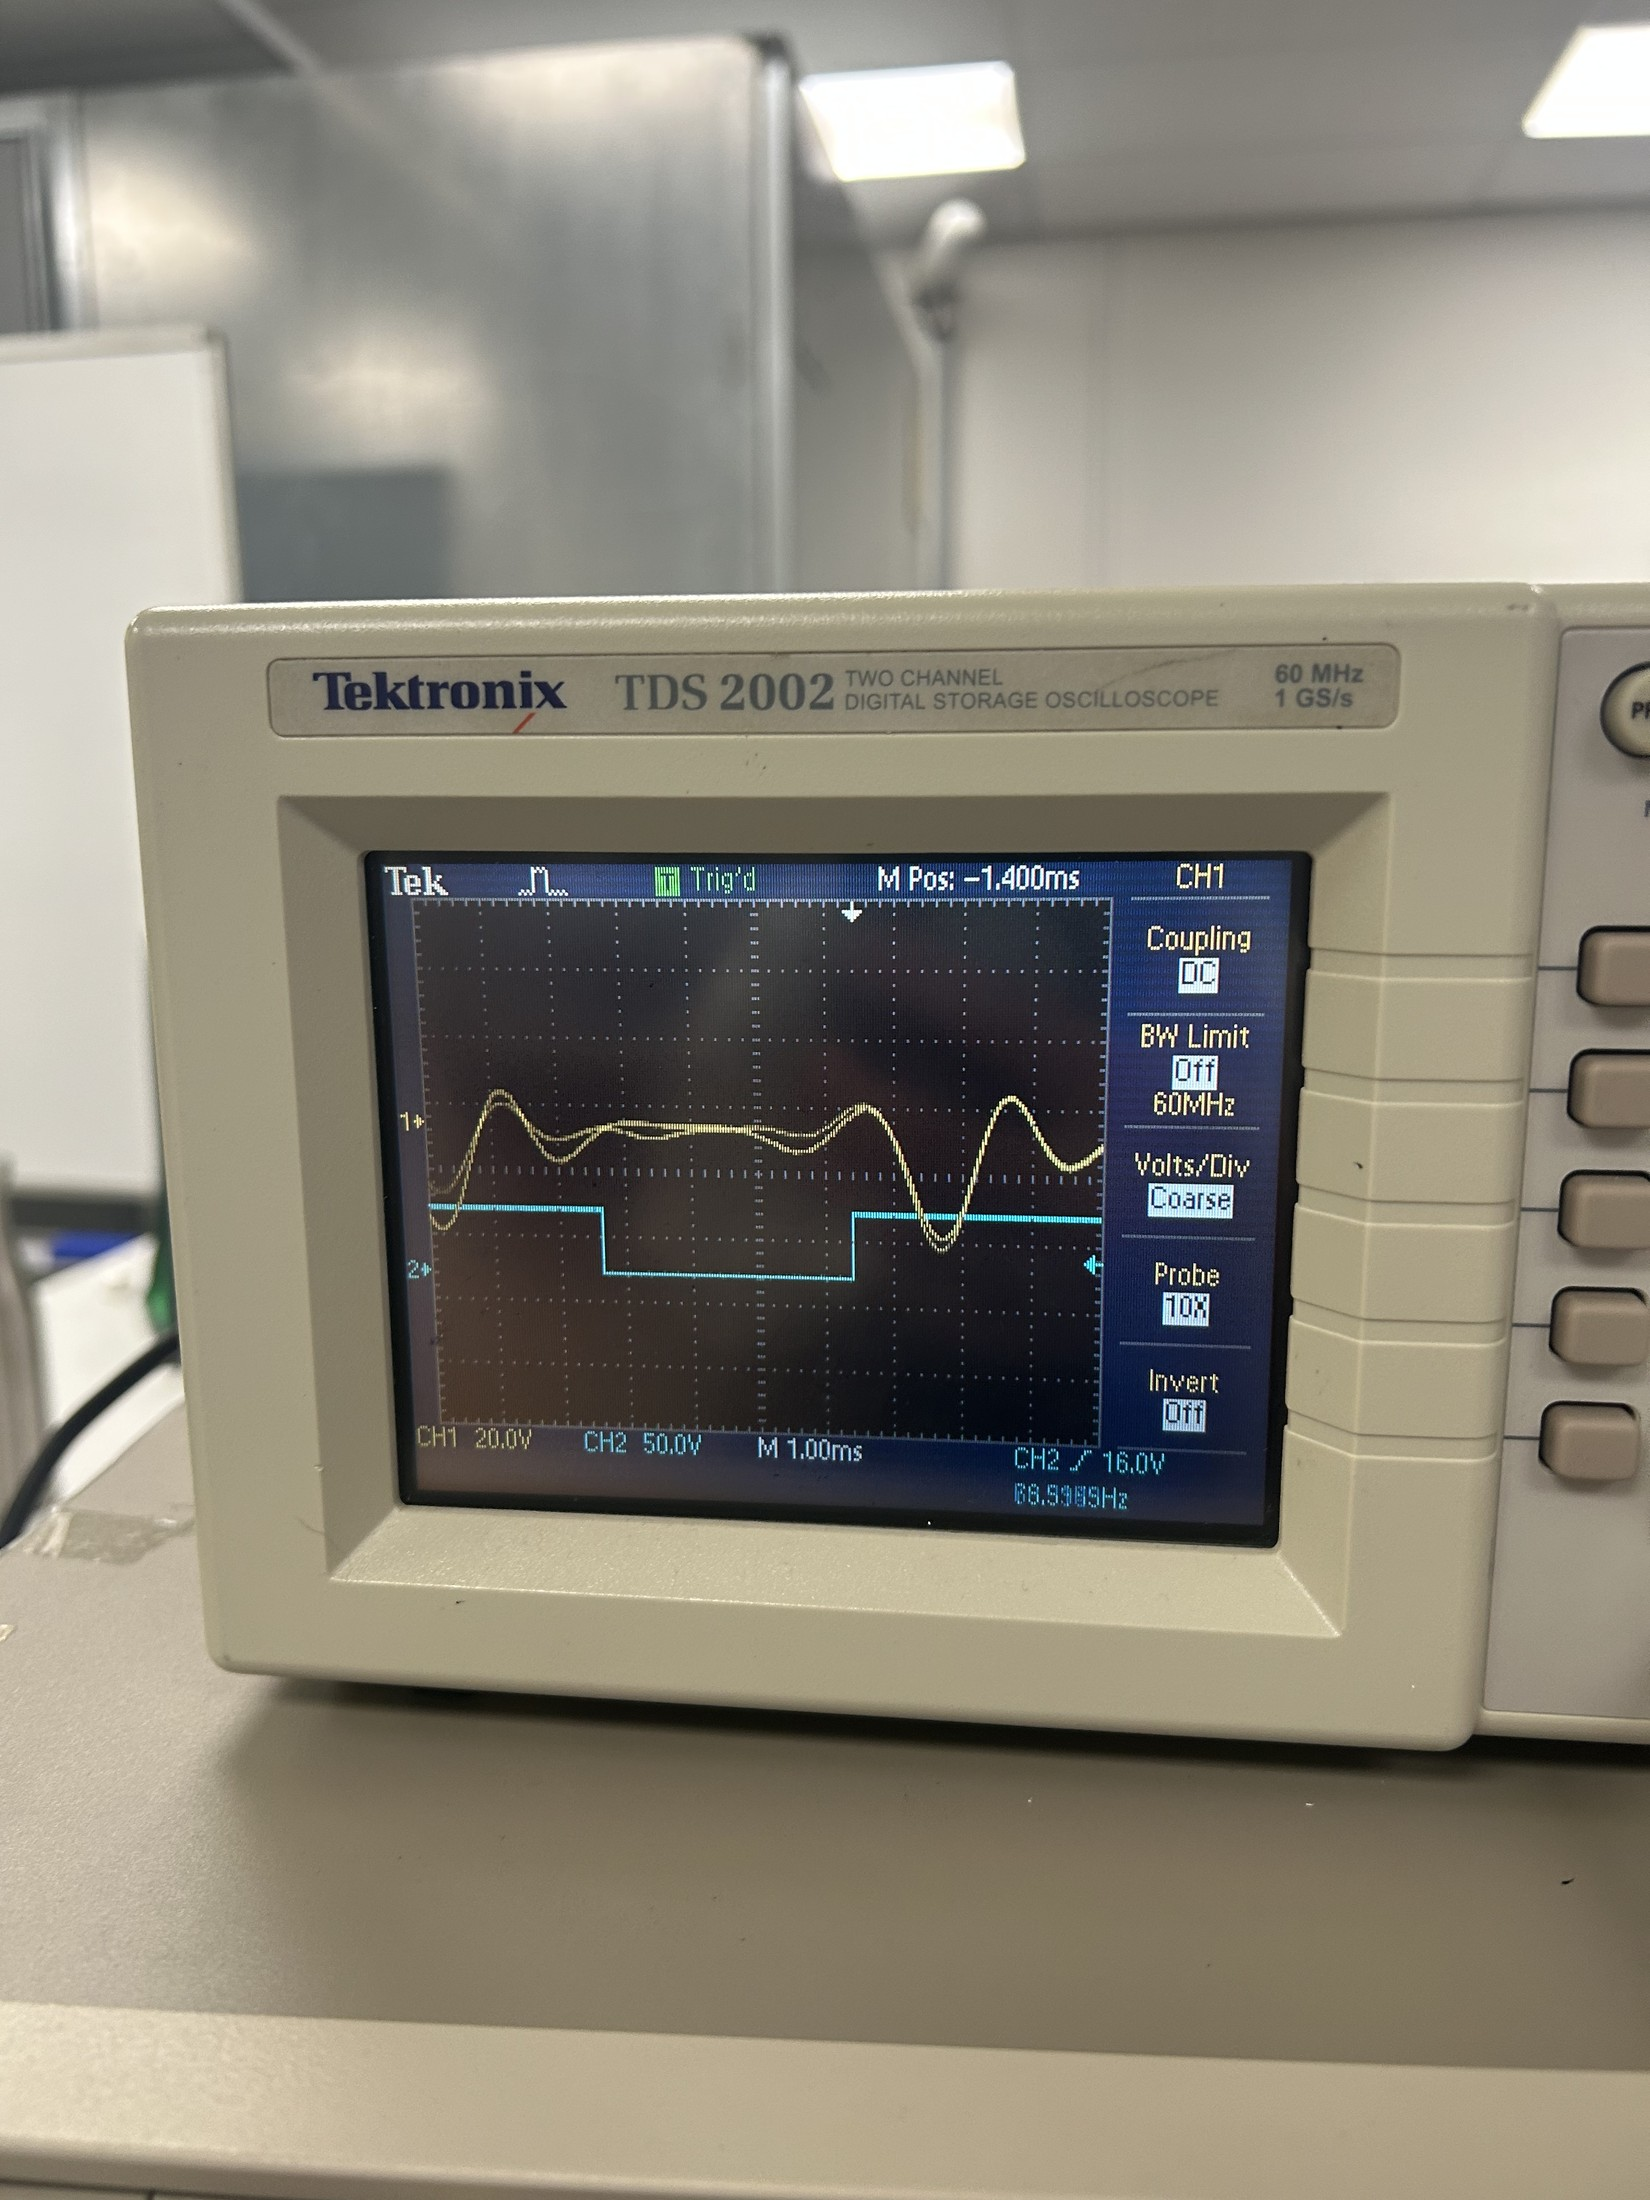
\includegraphics[width=\linewidth]{lab3_recovered_bandlimited_waveform.jpg}
\caption{A smoother recovered or filtered analogue waveform compared with a rectangular binary sequence.}
\end{subfigure}
\caption{Primary evidence that filtering changes transition shape and amplitude. The photos show rounded/oscillatory analogue transitions rather than a perfect rectangle. Exact probe points were not recorded, so the captions do not claim a more specific node than the images support.}
\label{fig:lab3-filtering}\end{figure}

\begin{observationbox}
Changing bandwidth visibly changed how sharply the analogue waveform followed the data. Reduced bandwidth suppressed fast edges and produced rounded transitions, ringing and amplitude changes. The decision stage therefore has to sample a filtered waveform at a suitable threshold rather than expect a perfect rectangular input.
\end{observationbox}

\subsection{Digital-related comparison}
\begin{figure}[H]\centering
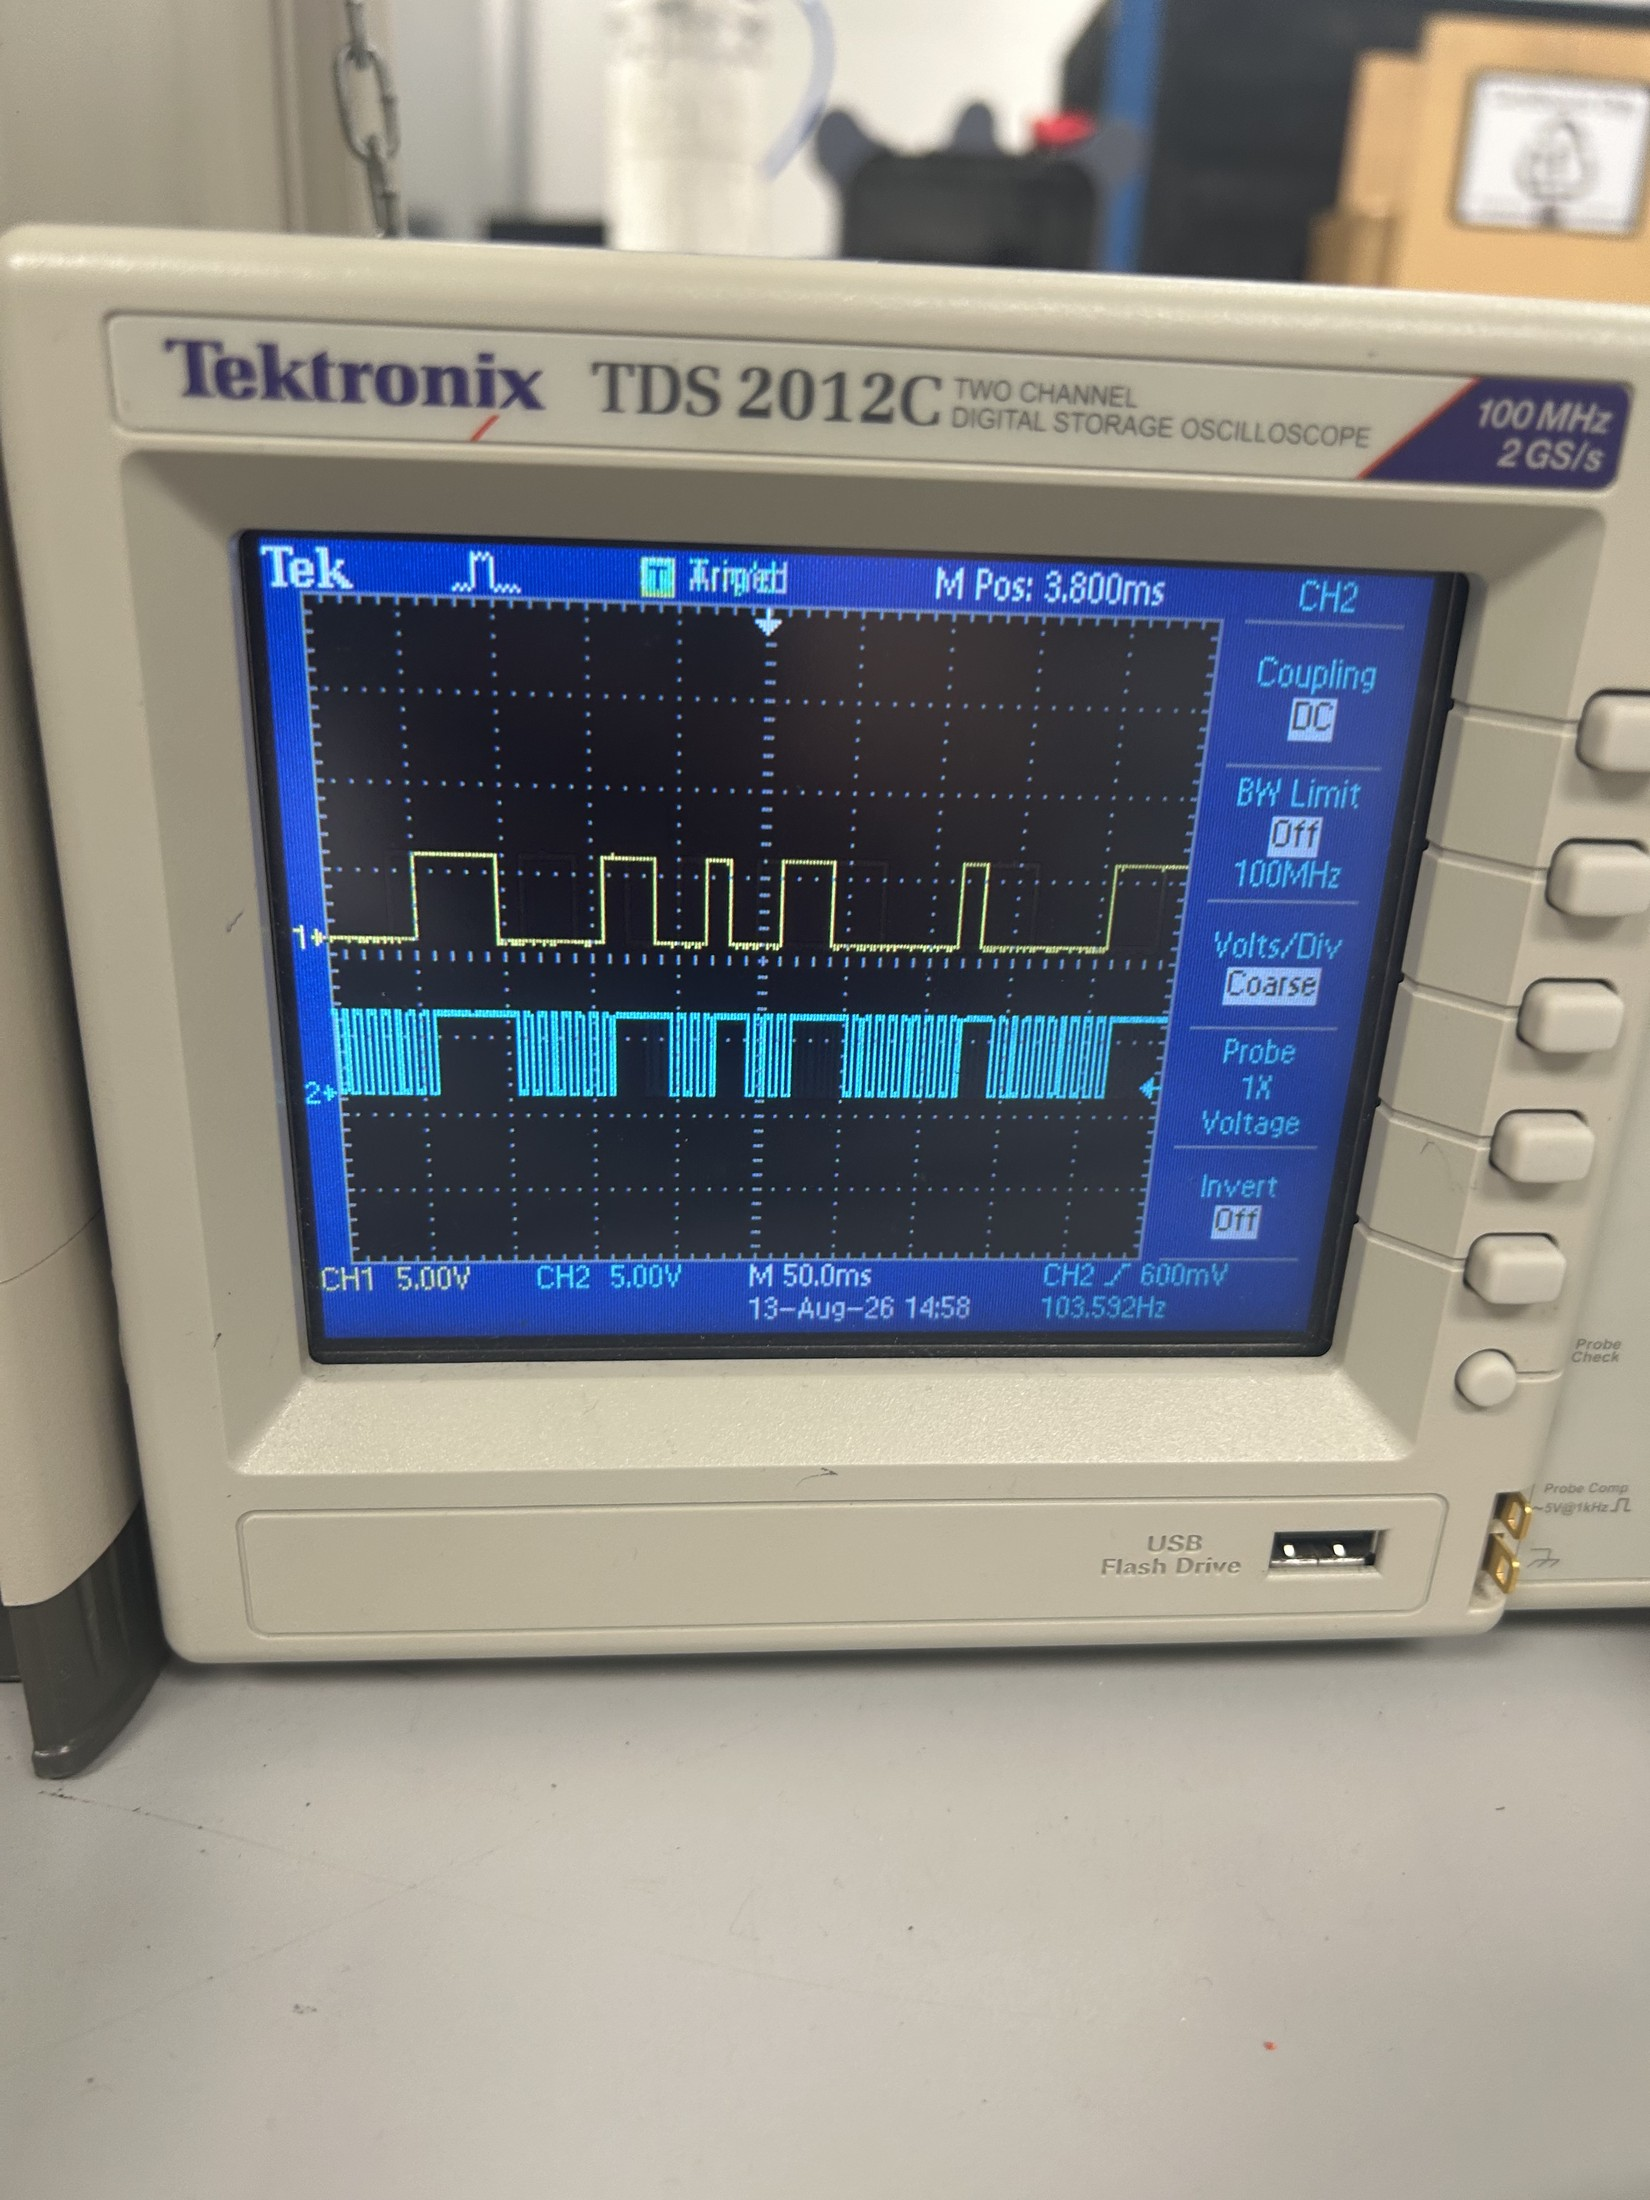
\includegraphics[width=0.60\textwidth]{lab3_digital_comparison.jpg}
\caption{Two simultaneously observed digital-related traces on the second oscilloscope. The display shows 5.00 V/div on both channels and 50.0 ms/div. The yellow trace is a slower binary pattern; the cyan trace contains groups of fast transitions associated with that pattern. This supports the presence of coordinated data/clock or line-code signals, but the exact probe-point mapping was not written down and is therefore left unclaimed.}
\label{fig:lab3-digital}\end{figure}

\begin{evidencebox}
Sixteen images were supplied. Two exact duplicate pairs were identified: \texttt{Image.jpeg}=\texttt{Image(1).jpeg} and \texttt{Image(3).jpeg}=\texttt{Image(4).jpeg}. The PDF uses five clear representatives. Several other photos repeat the same scope/setup states or crop away the useful trace, so they remain preserved outside the PDF but are not treated as additional independent results.
\end{evidencebox}

\subsection{Manual questions answered}
\subsubsection*{Question 1 -- Is BPSK an analogue signal?}
\begin{answerbox}
Yes, the transmitted BPSK waveform is an analogue continuous-time carrier waveform, even though it represents digital information. The binary symbol selects one of two carrier phases, normally separated by $180^\circ$. It is therefore best described as a digitally modulated analogue waveform, not as a baseband TTL signal.
\end{answerbox}

\subsubsection*{Question 2 -- Must the transmitter multiplier be set to DC?}
\begin{answerbox}
For this model it should be DC coupled. The bipolar NRZ-L data can contain low-frequency content and long constant runs. AC coupling would remove the DC/very-low-frequency component, introduce baseline droop and distort the multiplier input, especially across long runs. DC coupling preserves the intended positive and negative data levels that select the two BPSK phases.
\end{answerbox}

\subsubsection*{Question 3 -- Does changing receiver phase-shifter setting influence the BPSK spectrum?}
\begin{answerbox}
Changing the receiver's local-carrier phase does not change the spectrum of the already-transmitted BPSK signal. It changes the coherent demodulator result: the recovered baseband amplitude can reduce, reverse sign or pass through zero as the local carrier moves away from the correct phase. A phase change applied at the transmitter would alter absolute phase, but a constant phase rotation does not change the magnitude spectrum.
\end{answerbox}

\subsubsection*{Question 4 -- Does making bit rate a sub-multiple of carrier frequency influence the spectrum?}
\begin{answerbox}
The principal occupied bandwidth is governed by the bit rate and pulse shaping, not simply by choosing an integer carrier/bit-rate ratio. The harmonic relationship does make transitions occur at repeatable carrier phases and can change the detailed line structure of a repetitive laboratory sequence, but it does not remove the sidebands created by the data. Band limiting is still required.
\end{answerbox}

\subsubsection*{Question 5 -- Purpose and bandwidth of the demodulator LPF}
\begin{answerbox}
After coherent multiplication, the output contains the wanted baseband data term and an unwanted term around twice the carrier frequency. The low-pass filter removes the high-frequency product and noise while retaining enough baseband bandwidth for the bit transitions. Its bandwidth is therefore chosen from the data rate and pulse shape, the required transition fidelity and intersymbol interference, and the attenuation needed at the double-carrier component.
\end{answerbox}

\subsubsection*{Question 6 -- Why can a narrower transmitter bandwidth produce a larger decision-input amplitude?}
\begin{answerbox}
The amplitude at one instant is the vector sum of many spectral components. Widening the bandwidth does not guarantee that every component adds constructively at the decision instant; additional components can partly cancel existing ones. Narrowing the filter can also create ringing or overshoot and shift the time of the peak. The measured peak can therefore increase even while total passed bandwidth or energy decreases. The practical result is that the decision threshold and sampling instant must be checked whenever the transmitter filter changes.
\end{answerbox}

\subsection{What remains uncertain}
\begin{checkbox}
*** I still need the session attendance/roles and the short weekly note. I also need confirmation of which exact nodes were connected to the two channels in Figures~\ref{fig:lab3-filtering} and~\ref{fig:lab3-digital} if we want captions more specific than the photographs support.
\end{checkbox}
\weeklynote{\textbf{Date:} ***\\\textbf{Who attended / roles:} ***\\\textbf{What we achieved:} We built and observed the BPSK transmitter/receiver chain, compared carrier/data-related traces, and investigated filtering and recovered signals.\\\textbf{What was difficult:} ***\\\textbf{What I learned:} BPSK stores binary information in the carrier phase, and coherent recovery depends on carrier phase, filtering and the decision threshold.\\\textbf{Next improvement:} Record every probe point and scope setting beside each photo while still at the bench.}
\labdivider
\section{Lab 4 -- Pulse-Code Modulation}
\subsection{Open labbook questions}
\subsubsection*{Who attended Lab 4 with me?}
\begin{answerbox}
Nahil attended Lab 4 with me. The other two group members were sick, so Nahil and I completed the class work as a pair. We first worked out how to read the four data-bit positions in the PCM frame, checked our interpretation with the lecturer and nearby classmates, and then divided the task between changing the input and recording each voltage/code pair.
\end{answerbox}

\subsubsection*{Are $-0.308$ V and $-0.270$ V exact values?}
\begin{answerbox}
They are the values preserved in my typed class-data transcription, but none of the retained meter photographs shows either value. I cannot independently confirm them from the surviving evidence. I have therefore plotted them exactly as recorded and highlighted them for checking rather than silently changing them. The $0.038$ V spacing between these adjacent codes is much smaller than the typical spacing in the rest of the linear table, so at least one of these entries may contain a transcription or measurement error.
\end{answerbox}

\subsubsection*{Were only 11 companded points measured?}
\begin{answerbox}
Only 11 companded points are preserved in the class-data file. The recorded decimal codes are 0, 1, 2, 3, 4, 9, 11, 12, 13, 14 and 15. Codes 5, 6, 7, 8 and 10 are absent. I found no second in-class table containing the missing values, so I describe the companded graph as partial rather than presenting it as a complete 16-level law.
\end{answerbox}

\subsubsection*{Can I confirm the evidence-photo grouping?}
\begin{answerbox}
Yes. The visible meter readings match the class-data table to within approximately 1 mV. The photographs at about $-2.634$, $-2.240$, $-1.911$ and $-1.595$ V match Question 4.1 codes 0000, 0001, 0010 and 0011. The photographs at about $-2.633$ and $-1.100$ V match Question 4.2 codes 0000 and 0001. Both photographs near $-2.63$ V show a minus sign; neither is evidence for the positive endpoint.
\end{answerbox}
\subsection{Evidence and measured graphs}
\begin{figure}[H]
\centering
\begin{subfigure}[t]{0.48\textwidth}
  \centering
  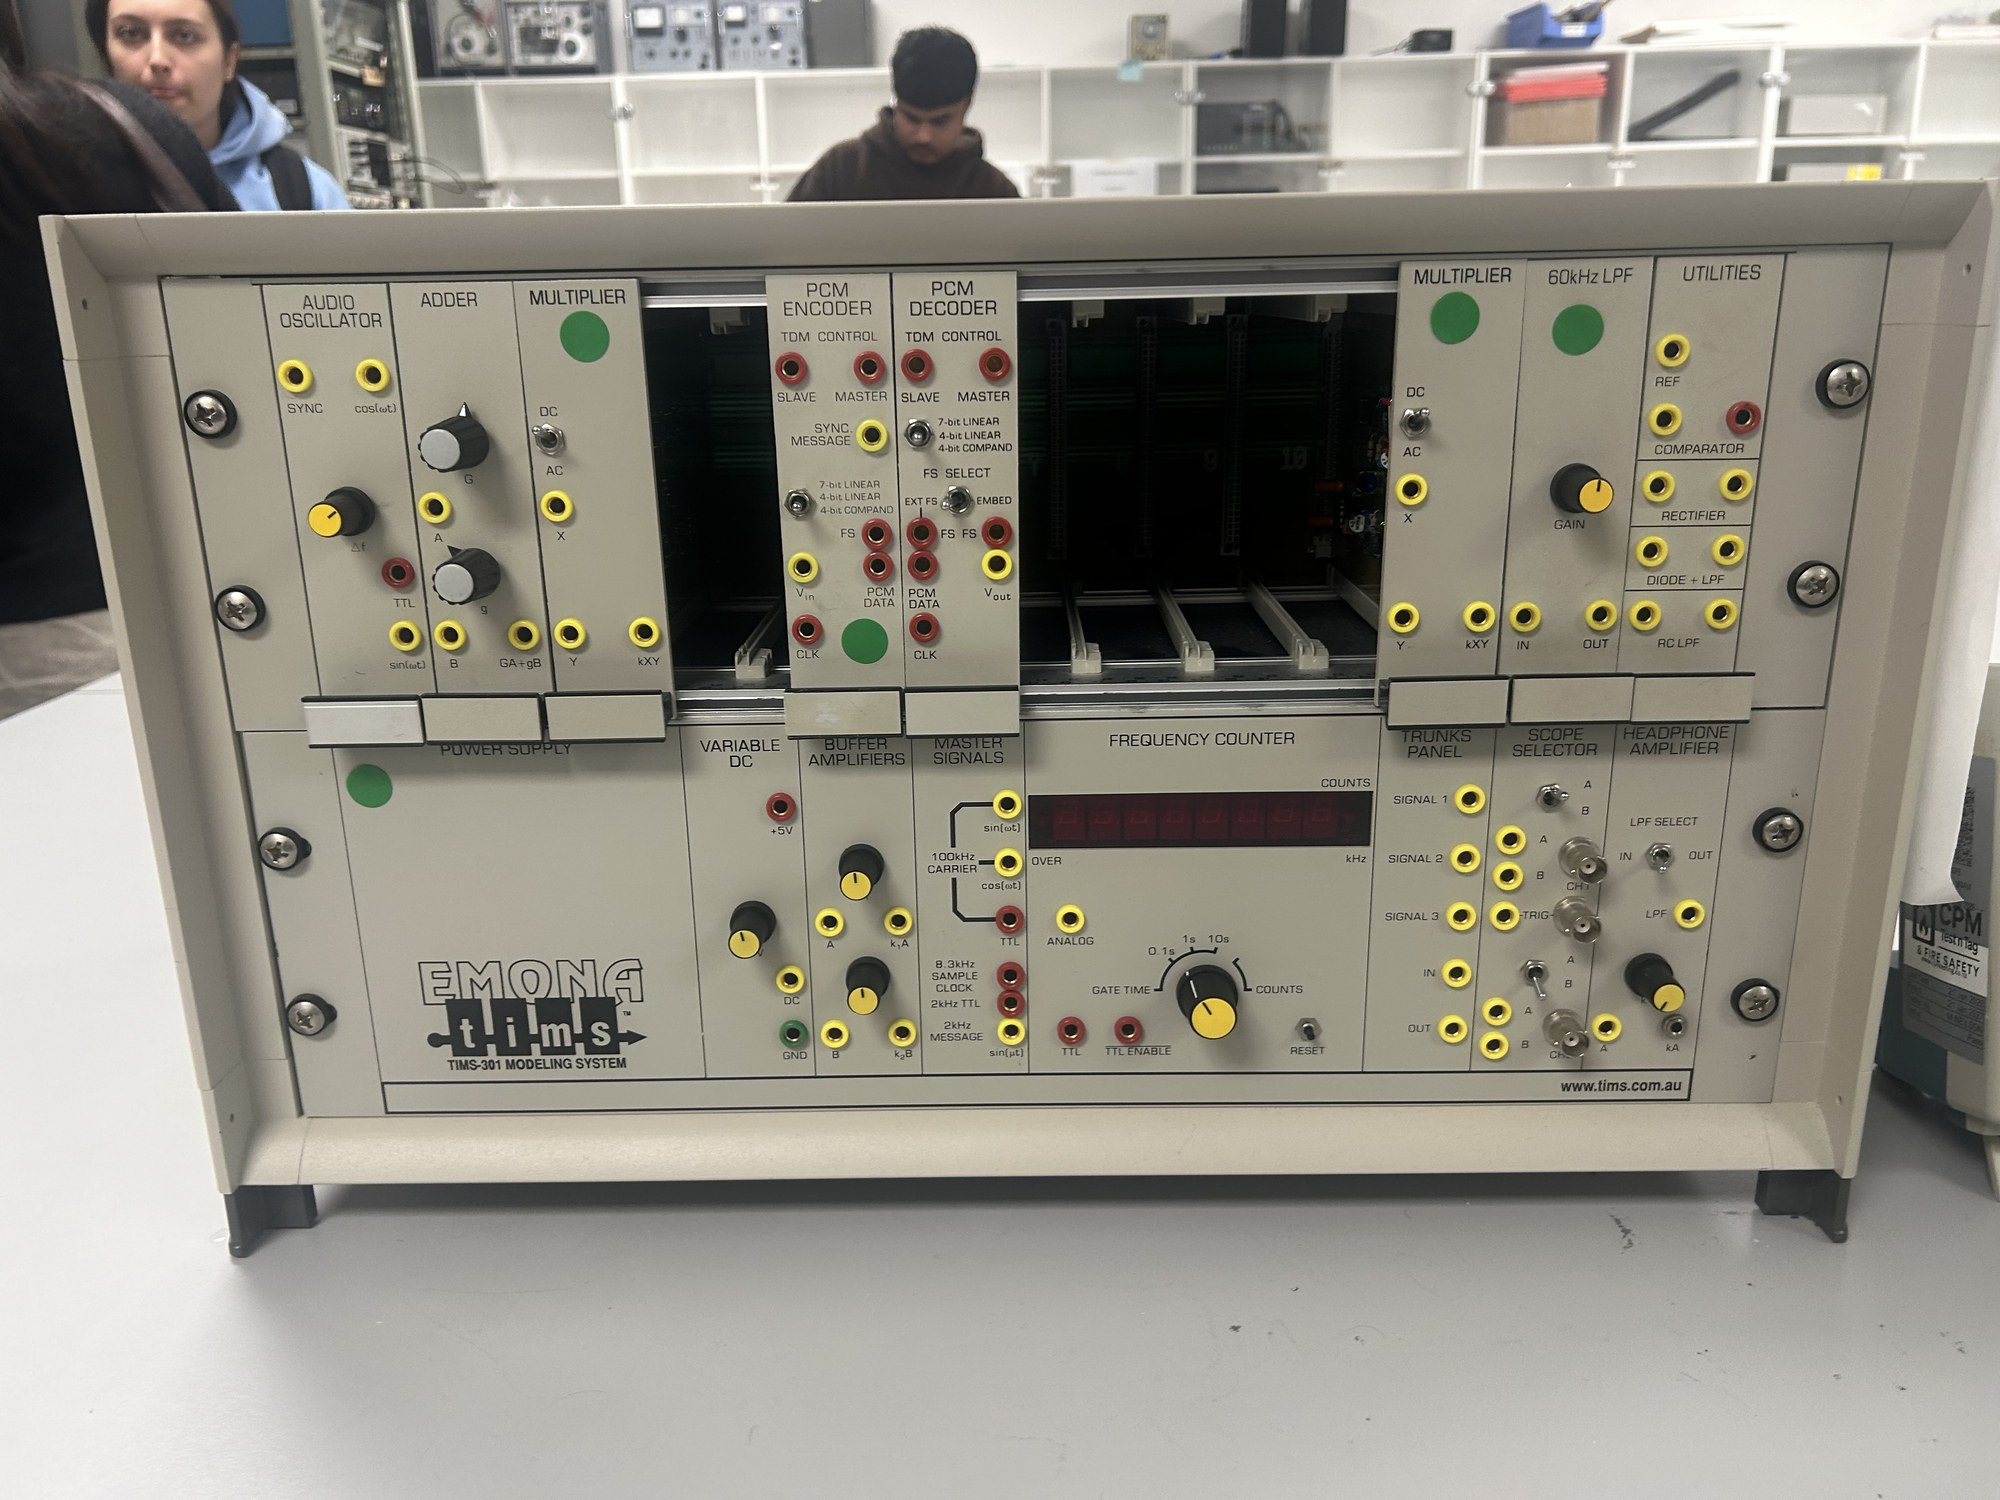
\includegraphics[width=\linewidth]{lab4_tims_system.jpg}
  \caption{The TIMS-301 system used in class.}
\end{subfigure}\hfill
\begin{subfigure}[t]{0.48\textwidth}
  \centering
  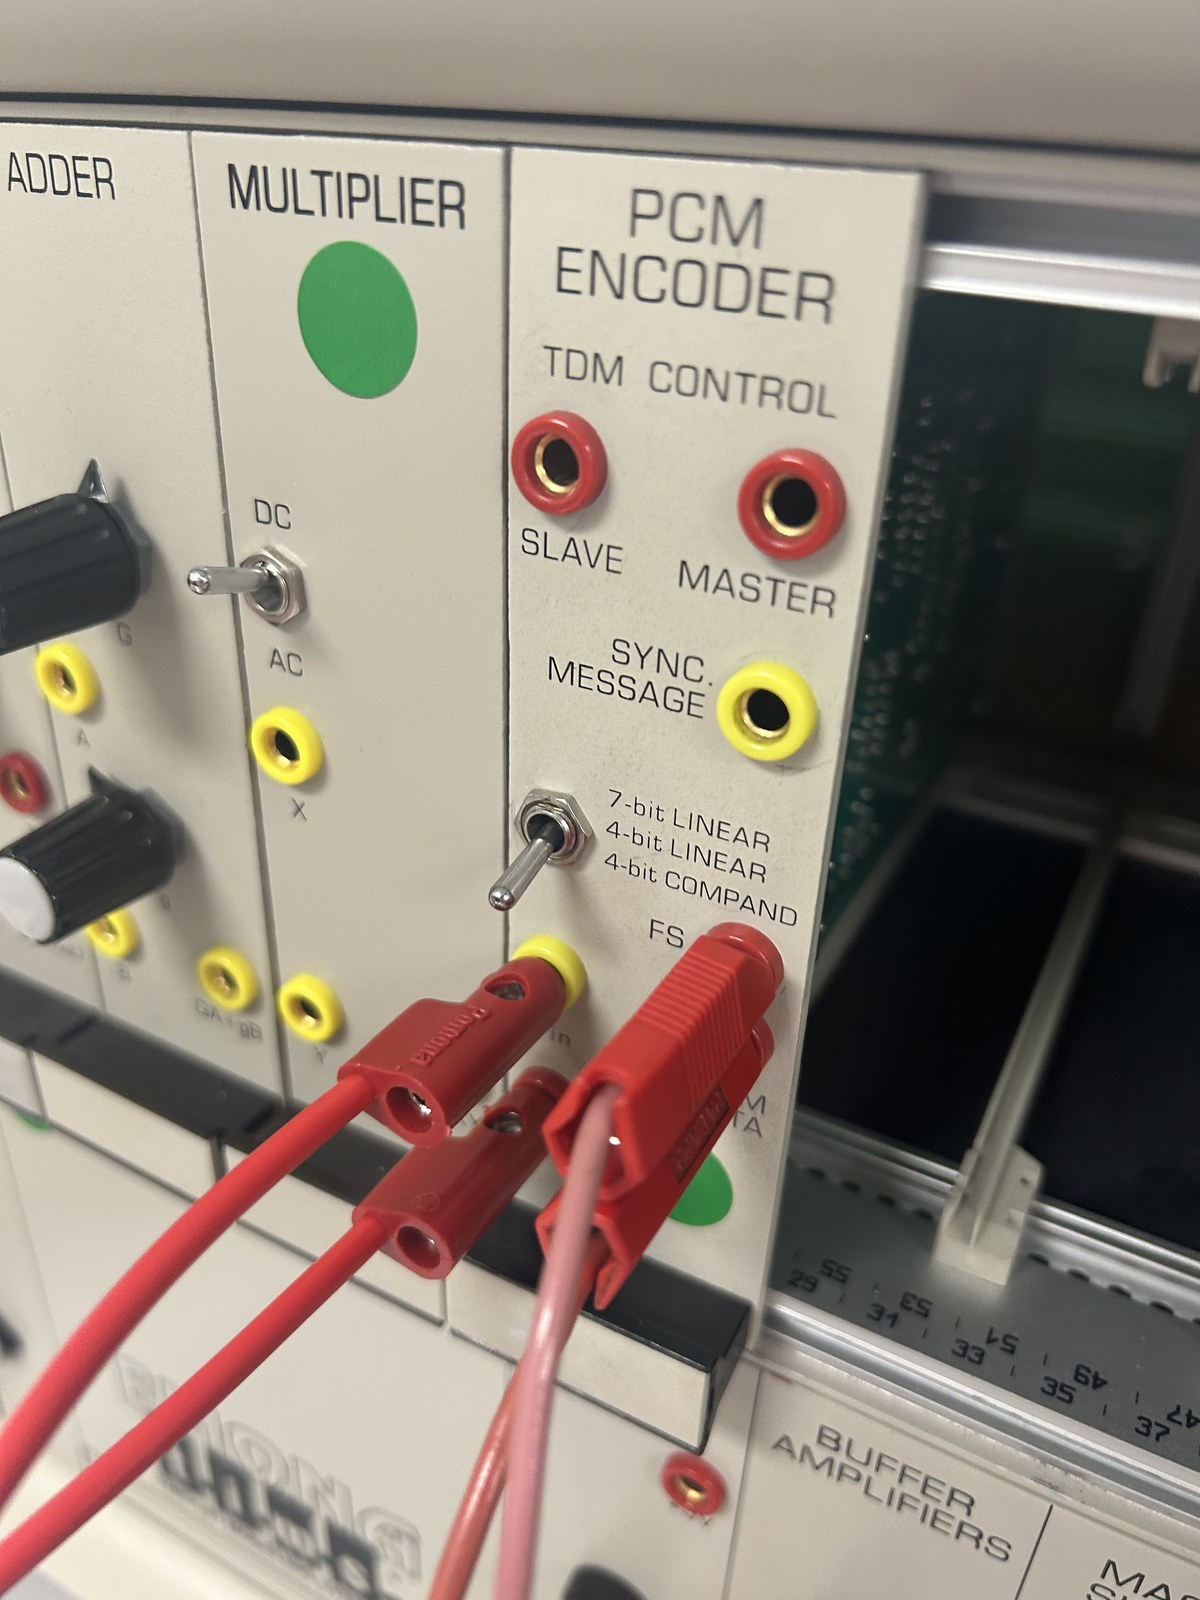
\includegraphics[width=\linewidth]{lab4_encoder_patch.jpg}
  \caption{Our in-class PCM encoder patching.}
\end{subfigure}
\caption{Primary physical evidence from Lab 4.}
\label{fig:lab4-setup}
\end{figure}

\begin{figure}[H]
  \centering
  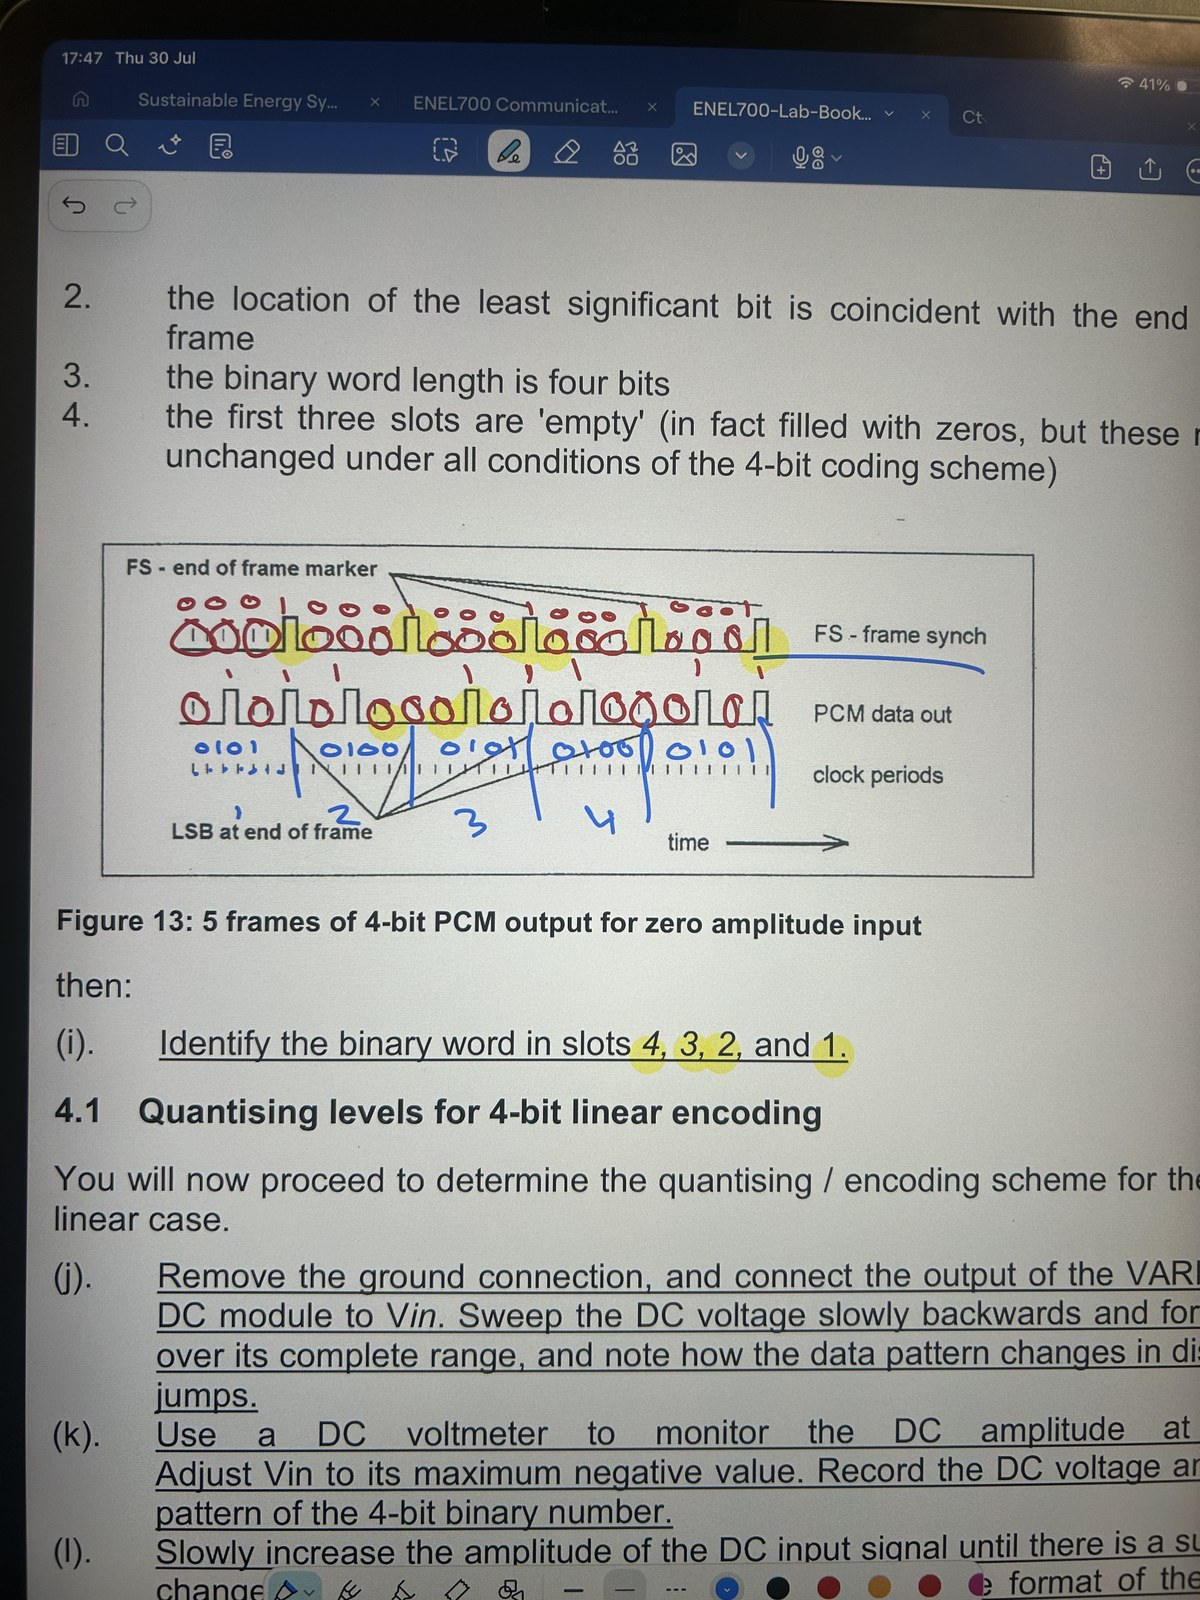
\includegraphics[width=0.55\textwidth]{lab4_decoding_note.jpg}
  \caption{Our in-class working note used to identify the four data-bit positions in each PCM frame.}
  \label{fig:lab4-note}
\end{figure}

\subsection{Question 4.1 raw linear data}

\begin{longtable}{r r c r}
\toprule
No. & $V_{in}$ (V) & Binary code & Decimal code \\
\midrule
\endhead
1 & $-2.635$ & 0000 & 0 \\
2 & $-2.239$ & 0001 & 1 \\
3 & $-1.911$ & 0010 & 2 \\
4 & $-1.595$ & 0011 & 3 \\
5 & $-1.277$ & 0100 & 4 \\
6 & $-0.960$ & 0101 & 5 \\
7 & $-0.308$ & 0110 & 6 \\
8 & $-0.270$ & 0111 & 7 \\
9 & $-0.020$ & 1000 & 8 \\
10 & $0.296$ & 1001 & 9 \\
11 & $0.645$ & 1010 & 10 \\
12 & $0.840$ & 1011 & 11 \\
13 & $1.314$ & 1100 & 12 \\
14 & $1.608$ & 1101 & 13 \\
15 & $2.062$ & 1110 & 14 \\
16 & $2.633$ & 1111 & 15 \\
\bottomrule
\end{longtable}

\begin{figure}[H]
  \centering
  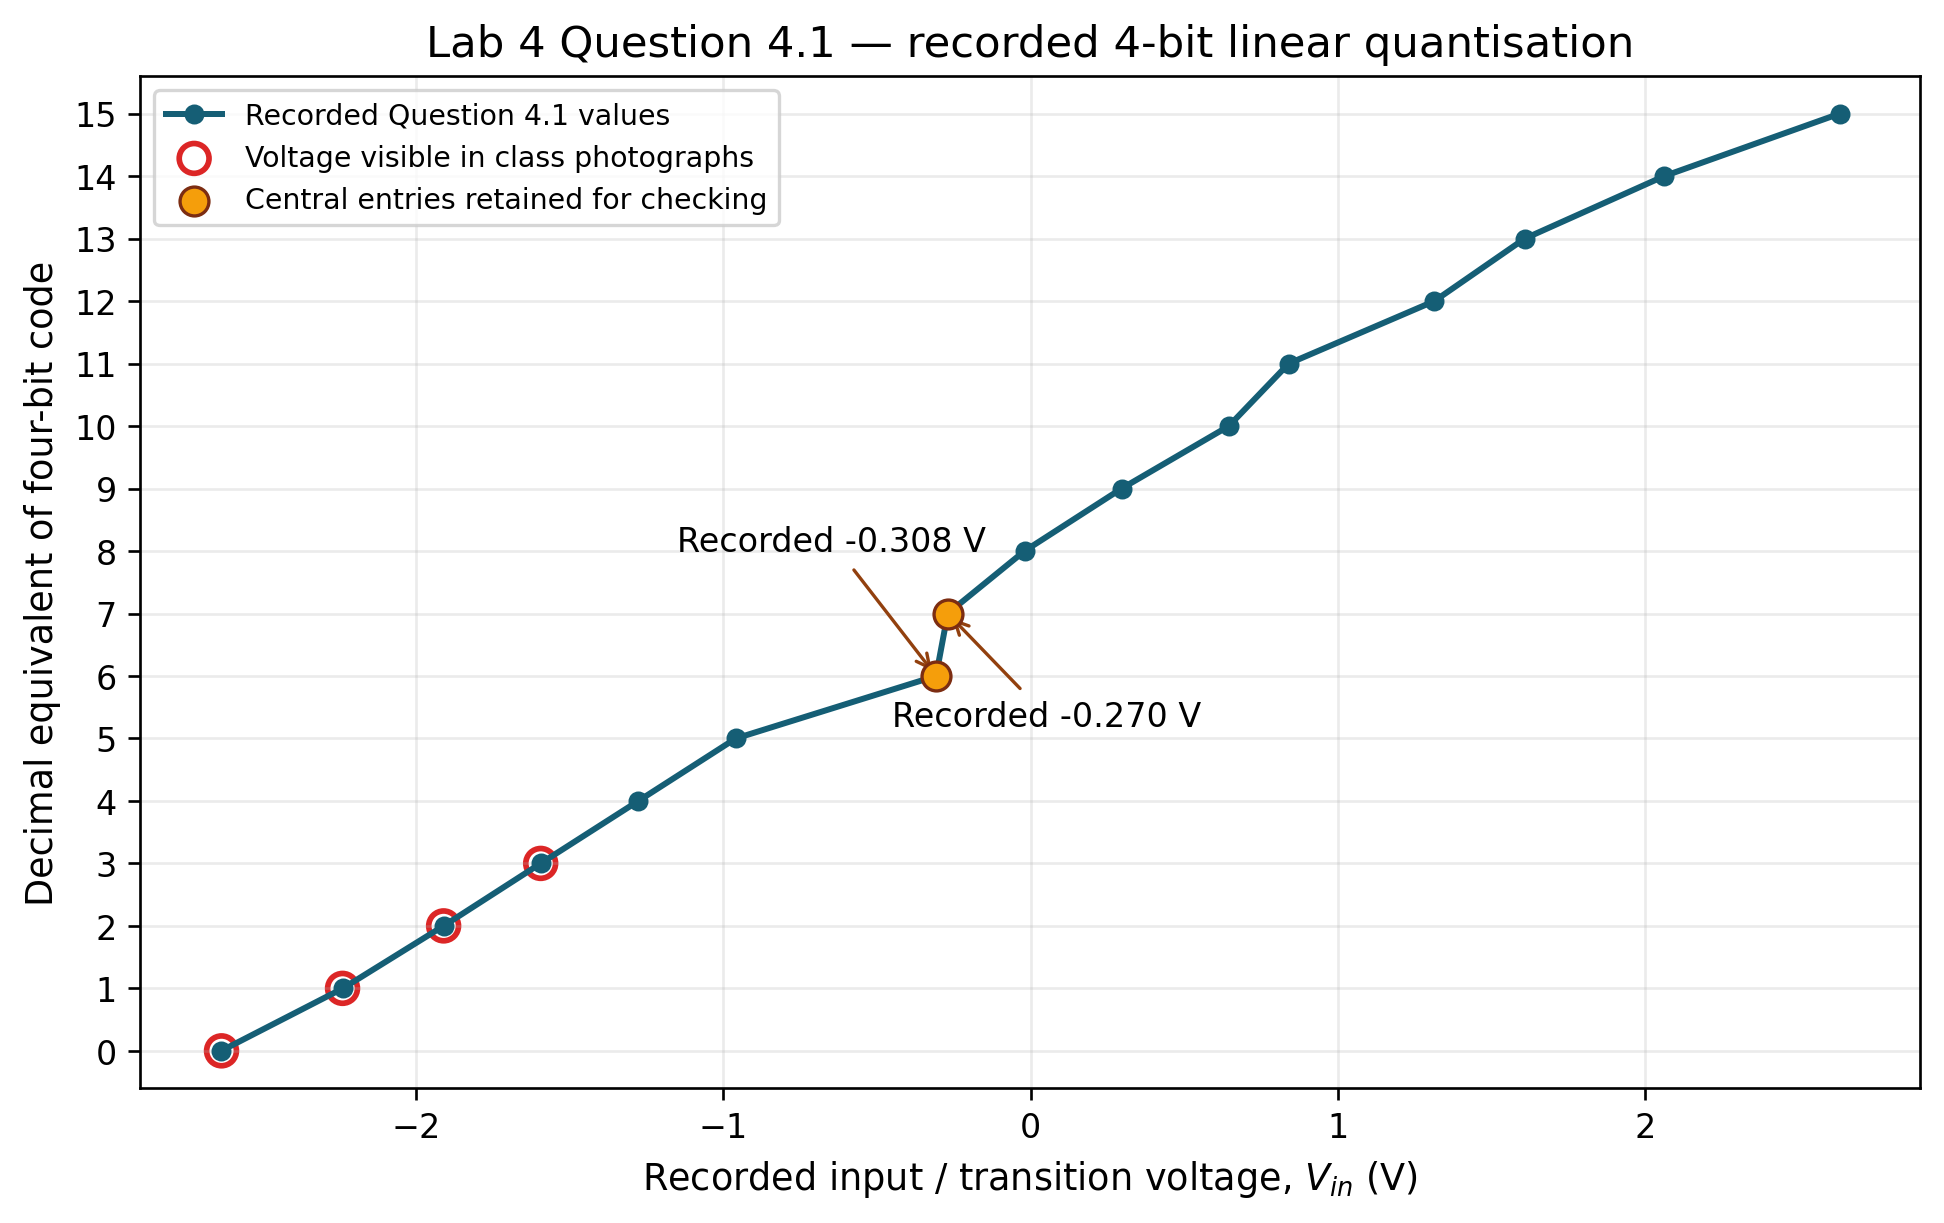
\includegraphics[width=0.96\textwidth]{lab4_q41_linear_raw.png}
  \caption{My graph of the Question 4.1 values exactly as recorded. The red rings mark values independently supported by class photographs. I retained the two questionable central entries and marked them in amber.}
  \label{fig:q41-linear}
\end{figure}

Across the full recorded range, the mean change is approximately $0.3512$ V per code step. The median adjacent spacing is approximately $0.318$ V. However, the recorded adjacent spacings range from $0.038$ V to $0.652$ V, largely because of the central entries. I therefore conclude that the result is broadly consistent with a linear 4-bit progression, but the typed table is not accurate enough to demonstrate uniform spacing quantitatively without checking the original hardcopy.

\begin{figure}[H]
\centering
\begin{subfigure}[t]{0.49\textwidth}
  \centering
  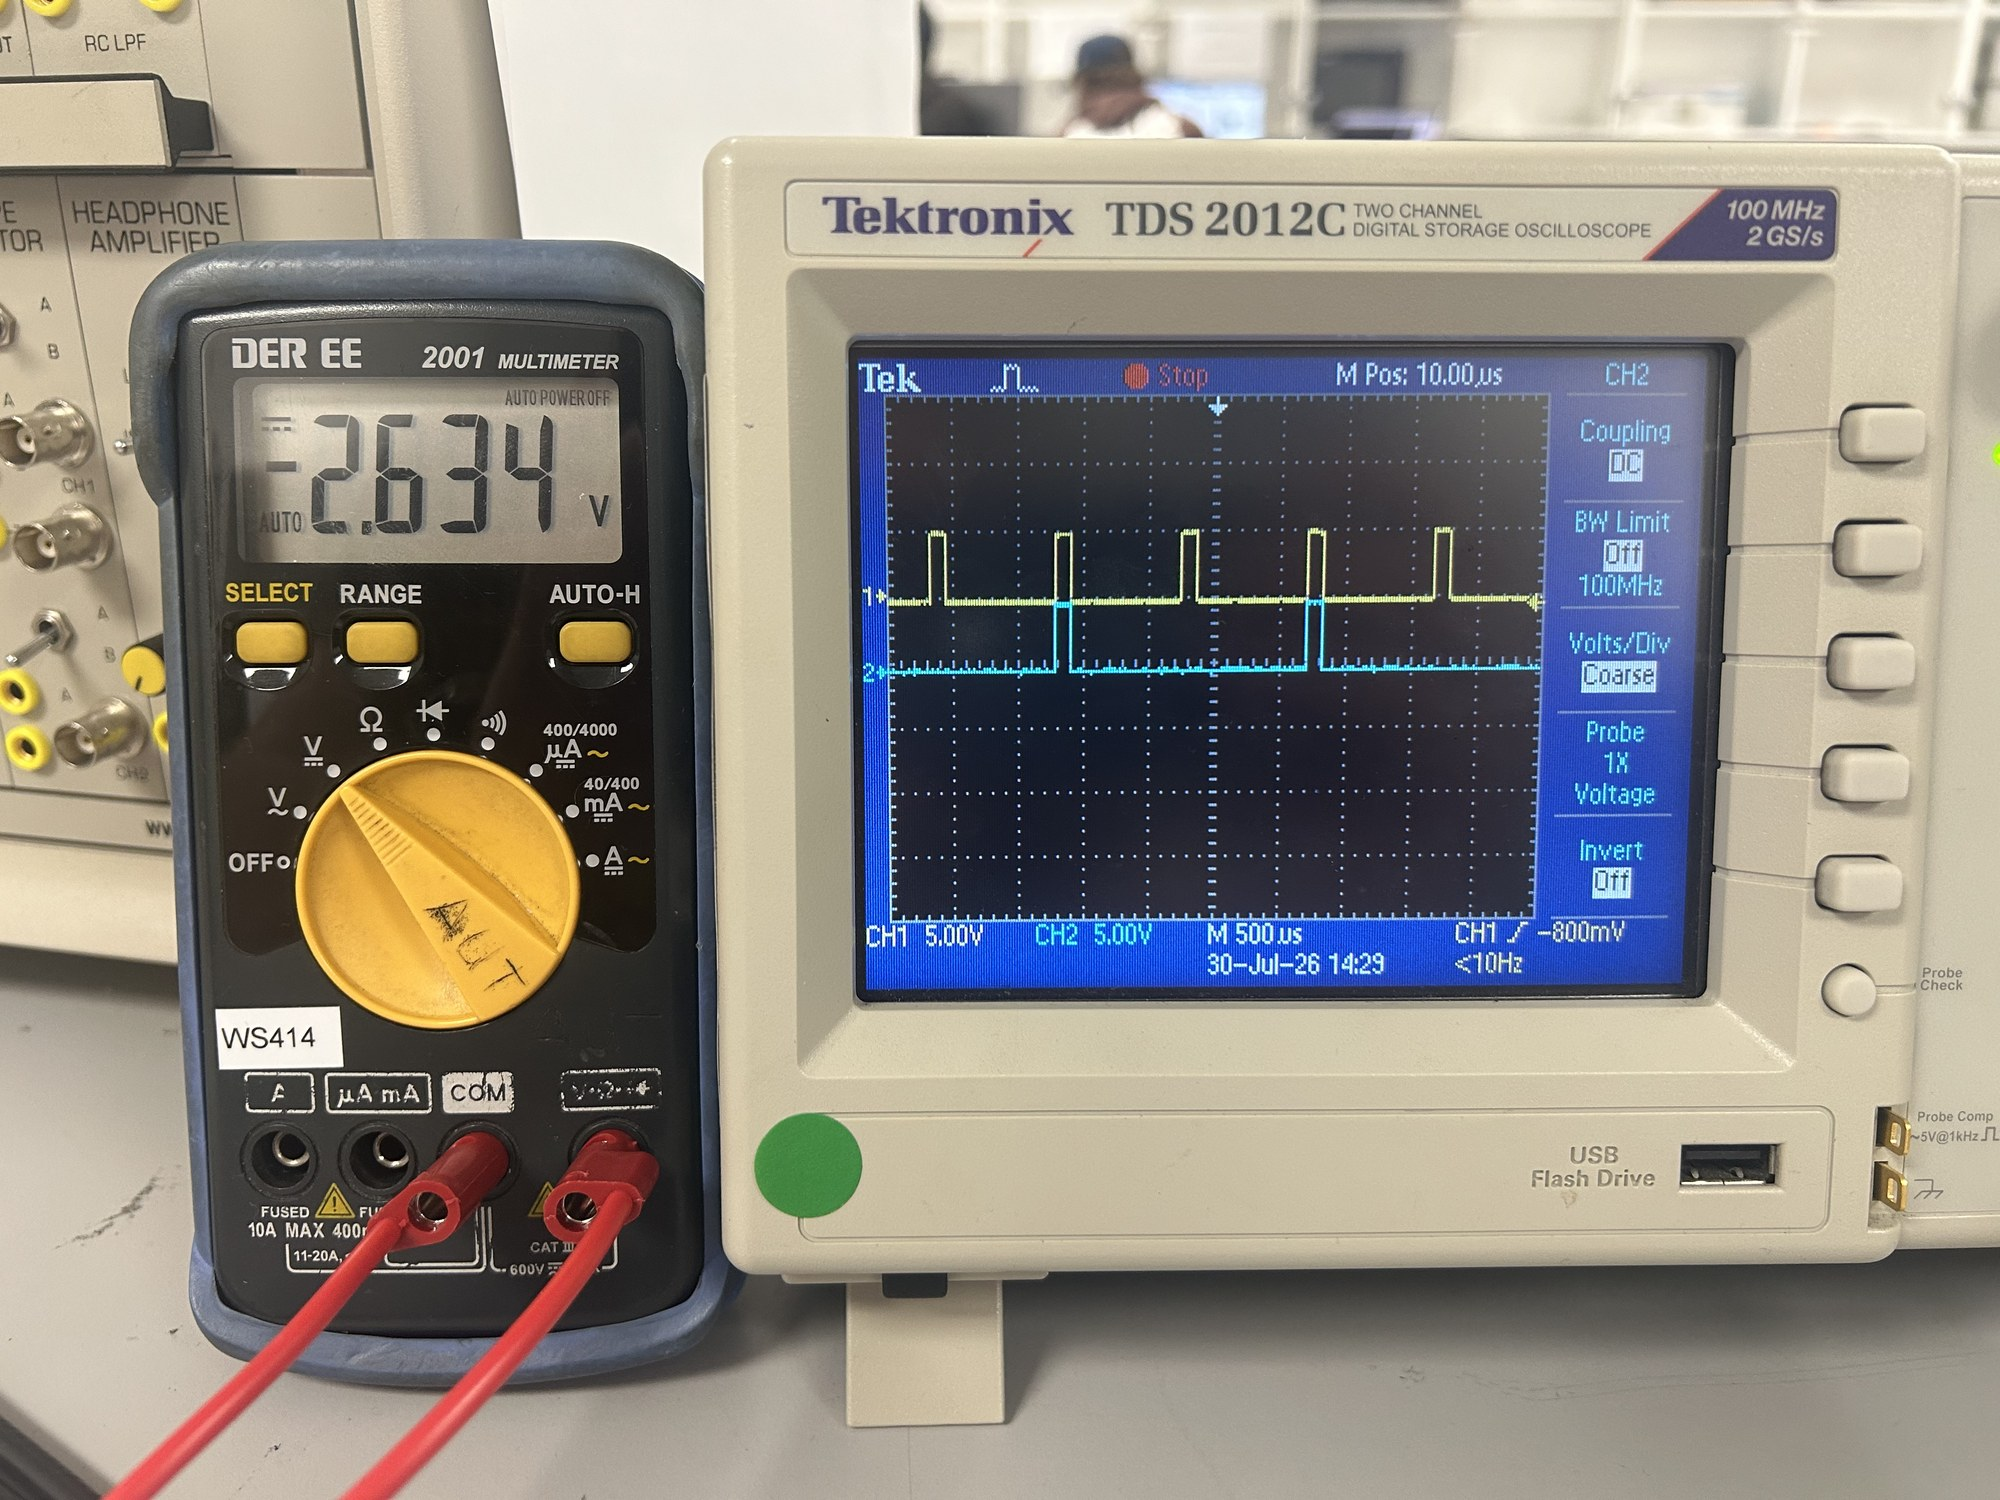
\includegraphics[width=\linewidth]{lab4_q41_minus2634.jpg}
  \caption{$-2.634$ V, code 0000.}
\end{subfigure}\hfill
\begin{subfigure}[t]{0.49\textwidth}
  \centering
  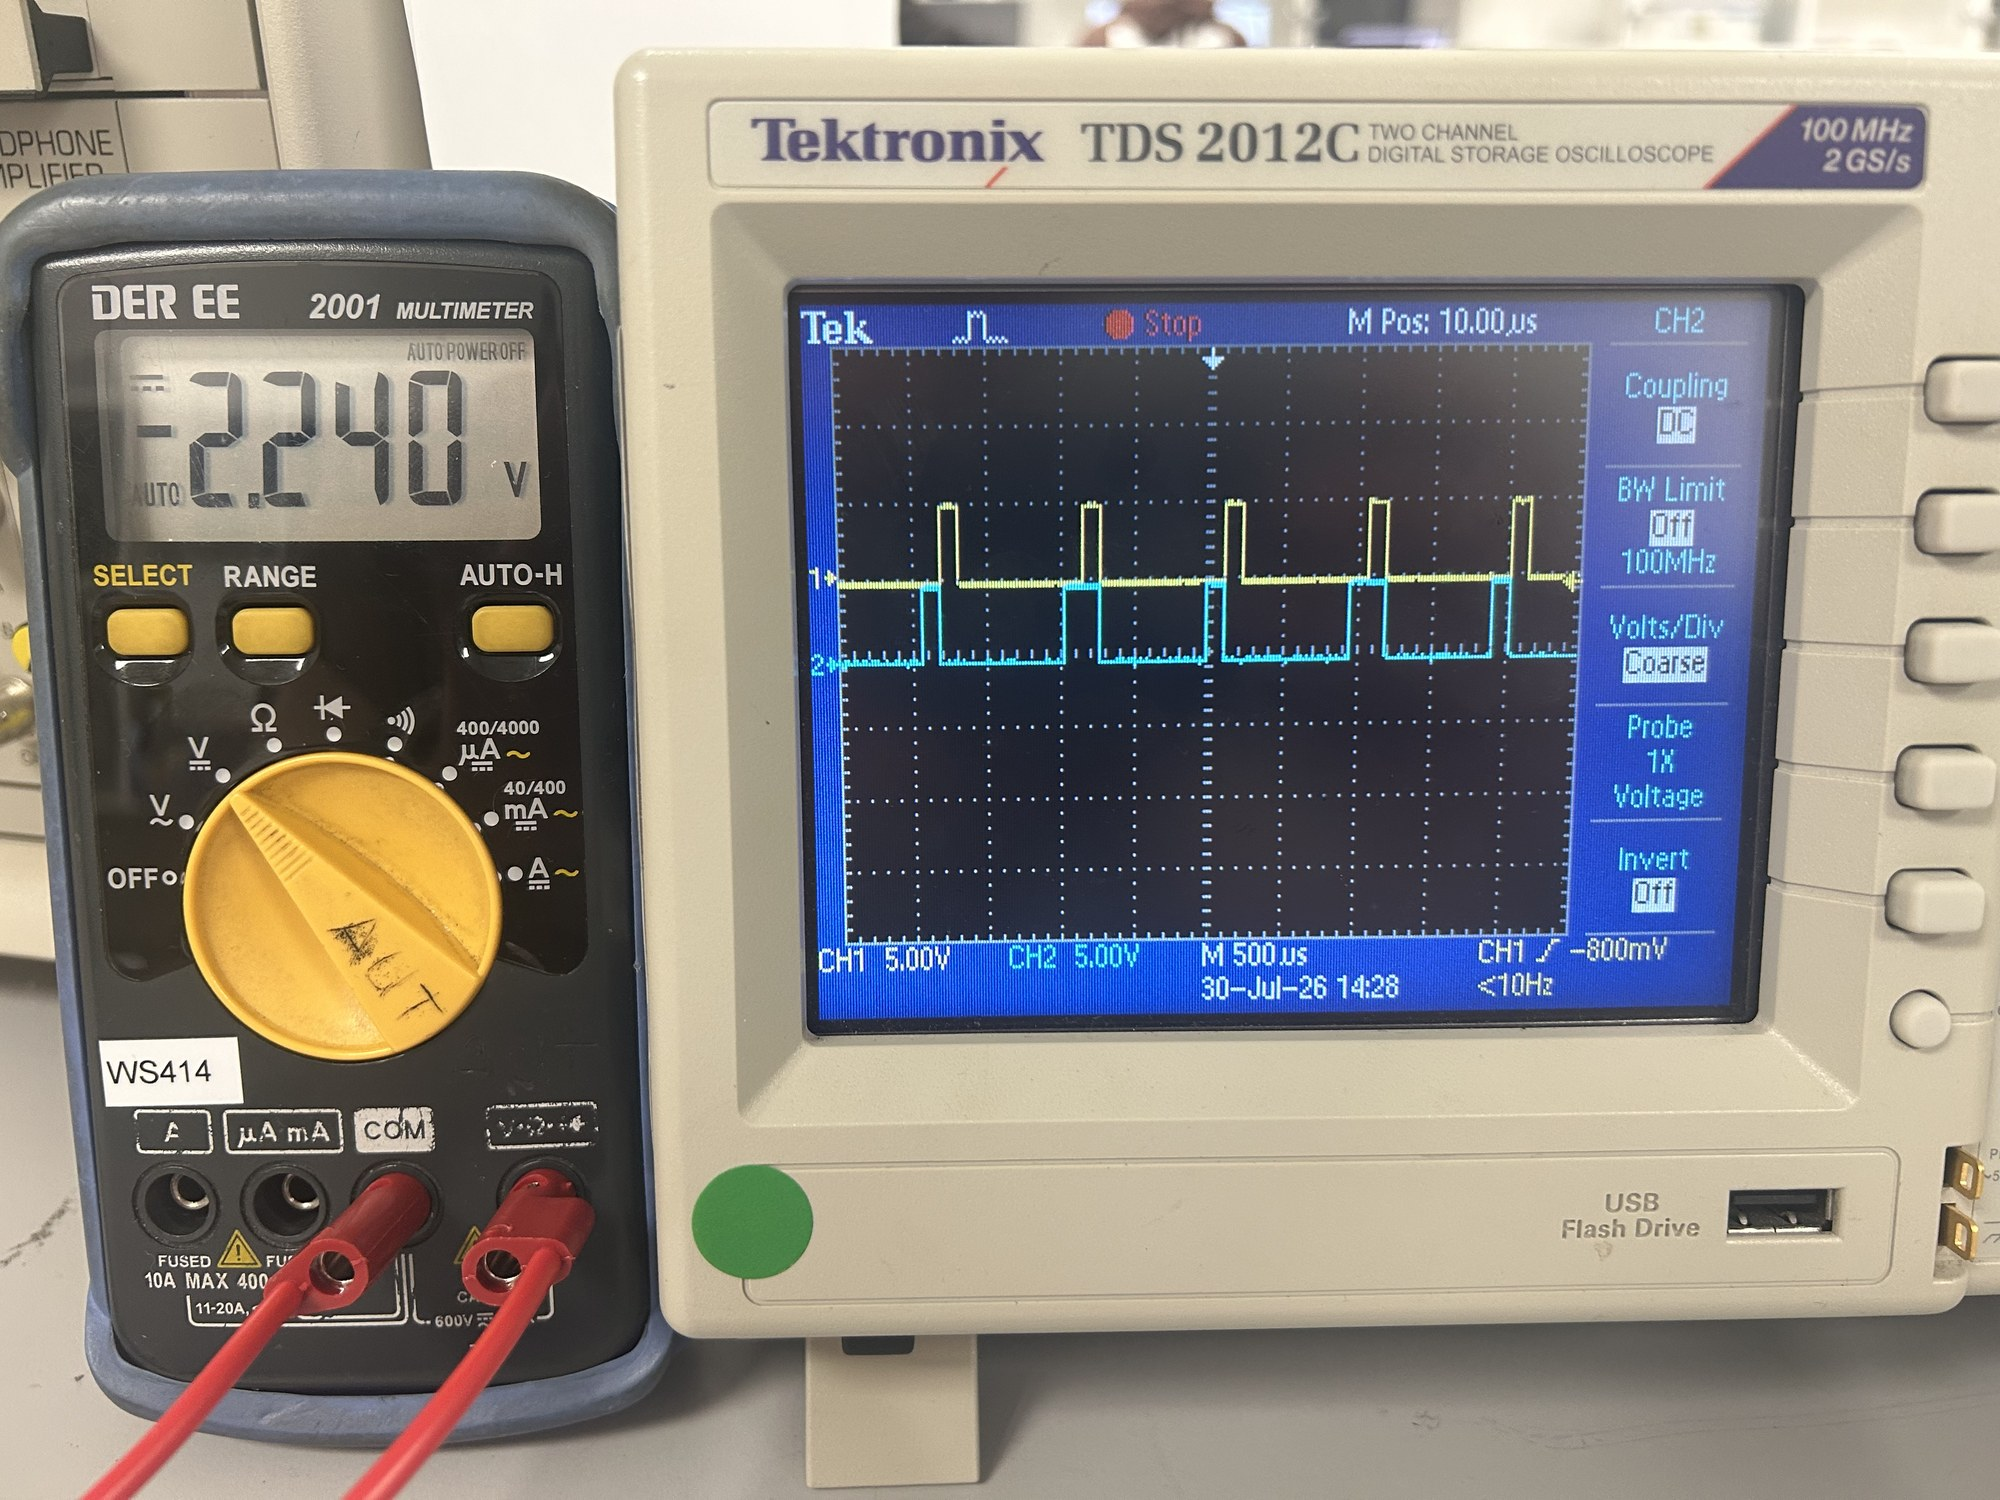
\includegraphics[width=\linewidth]{lab4_q41_minus2240.jpg}
  \caption{$-2.240$ V, code 0001.}
\end{subfigure}

\begin{subfigure}[t]{0.49\textwidth}
  \centering
  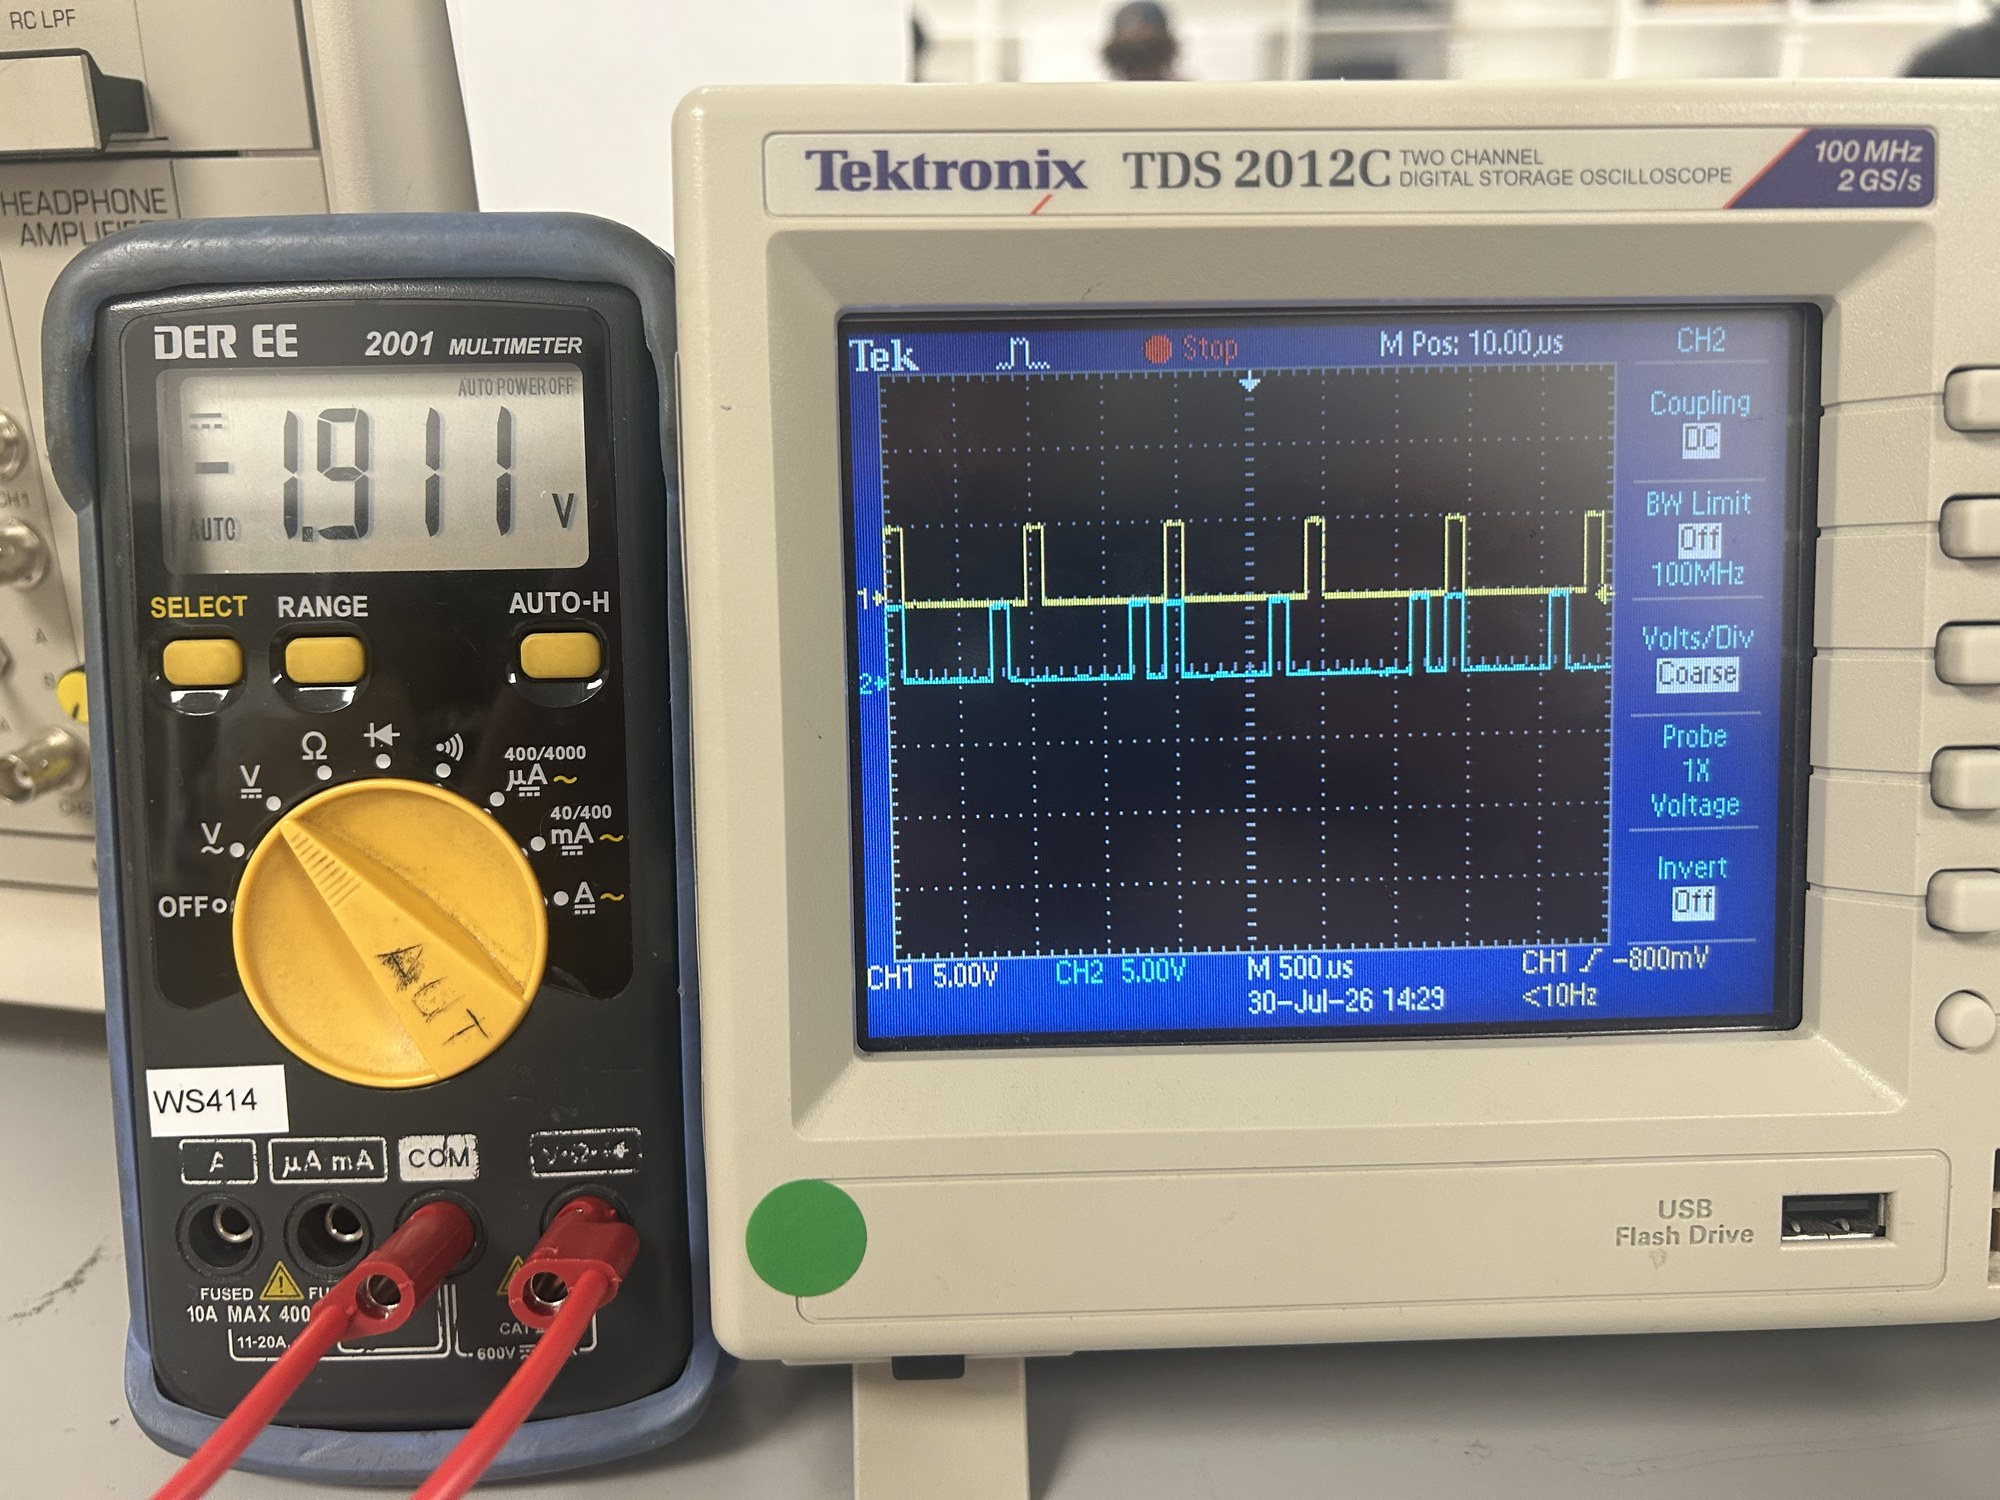
\includegraphics[width=\linewidth]{lab4_q41_minus1911.jpg}
  \caption{$-1.911$ V, code 0010.}
\end{subfigure}\hfill
\begin{subfigure}[t]{0.49\textwidth}
  \centering
  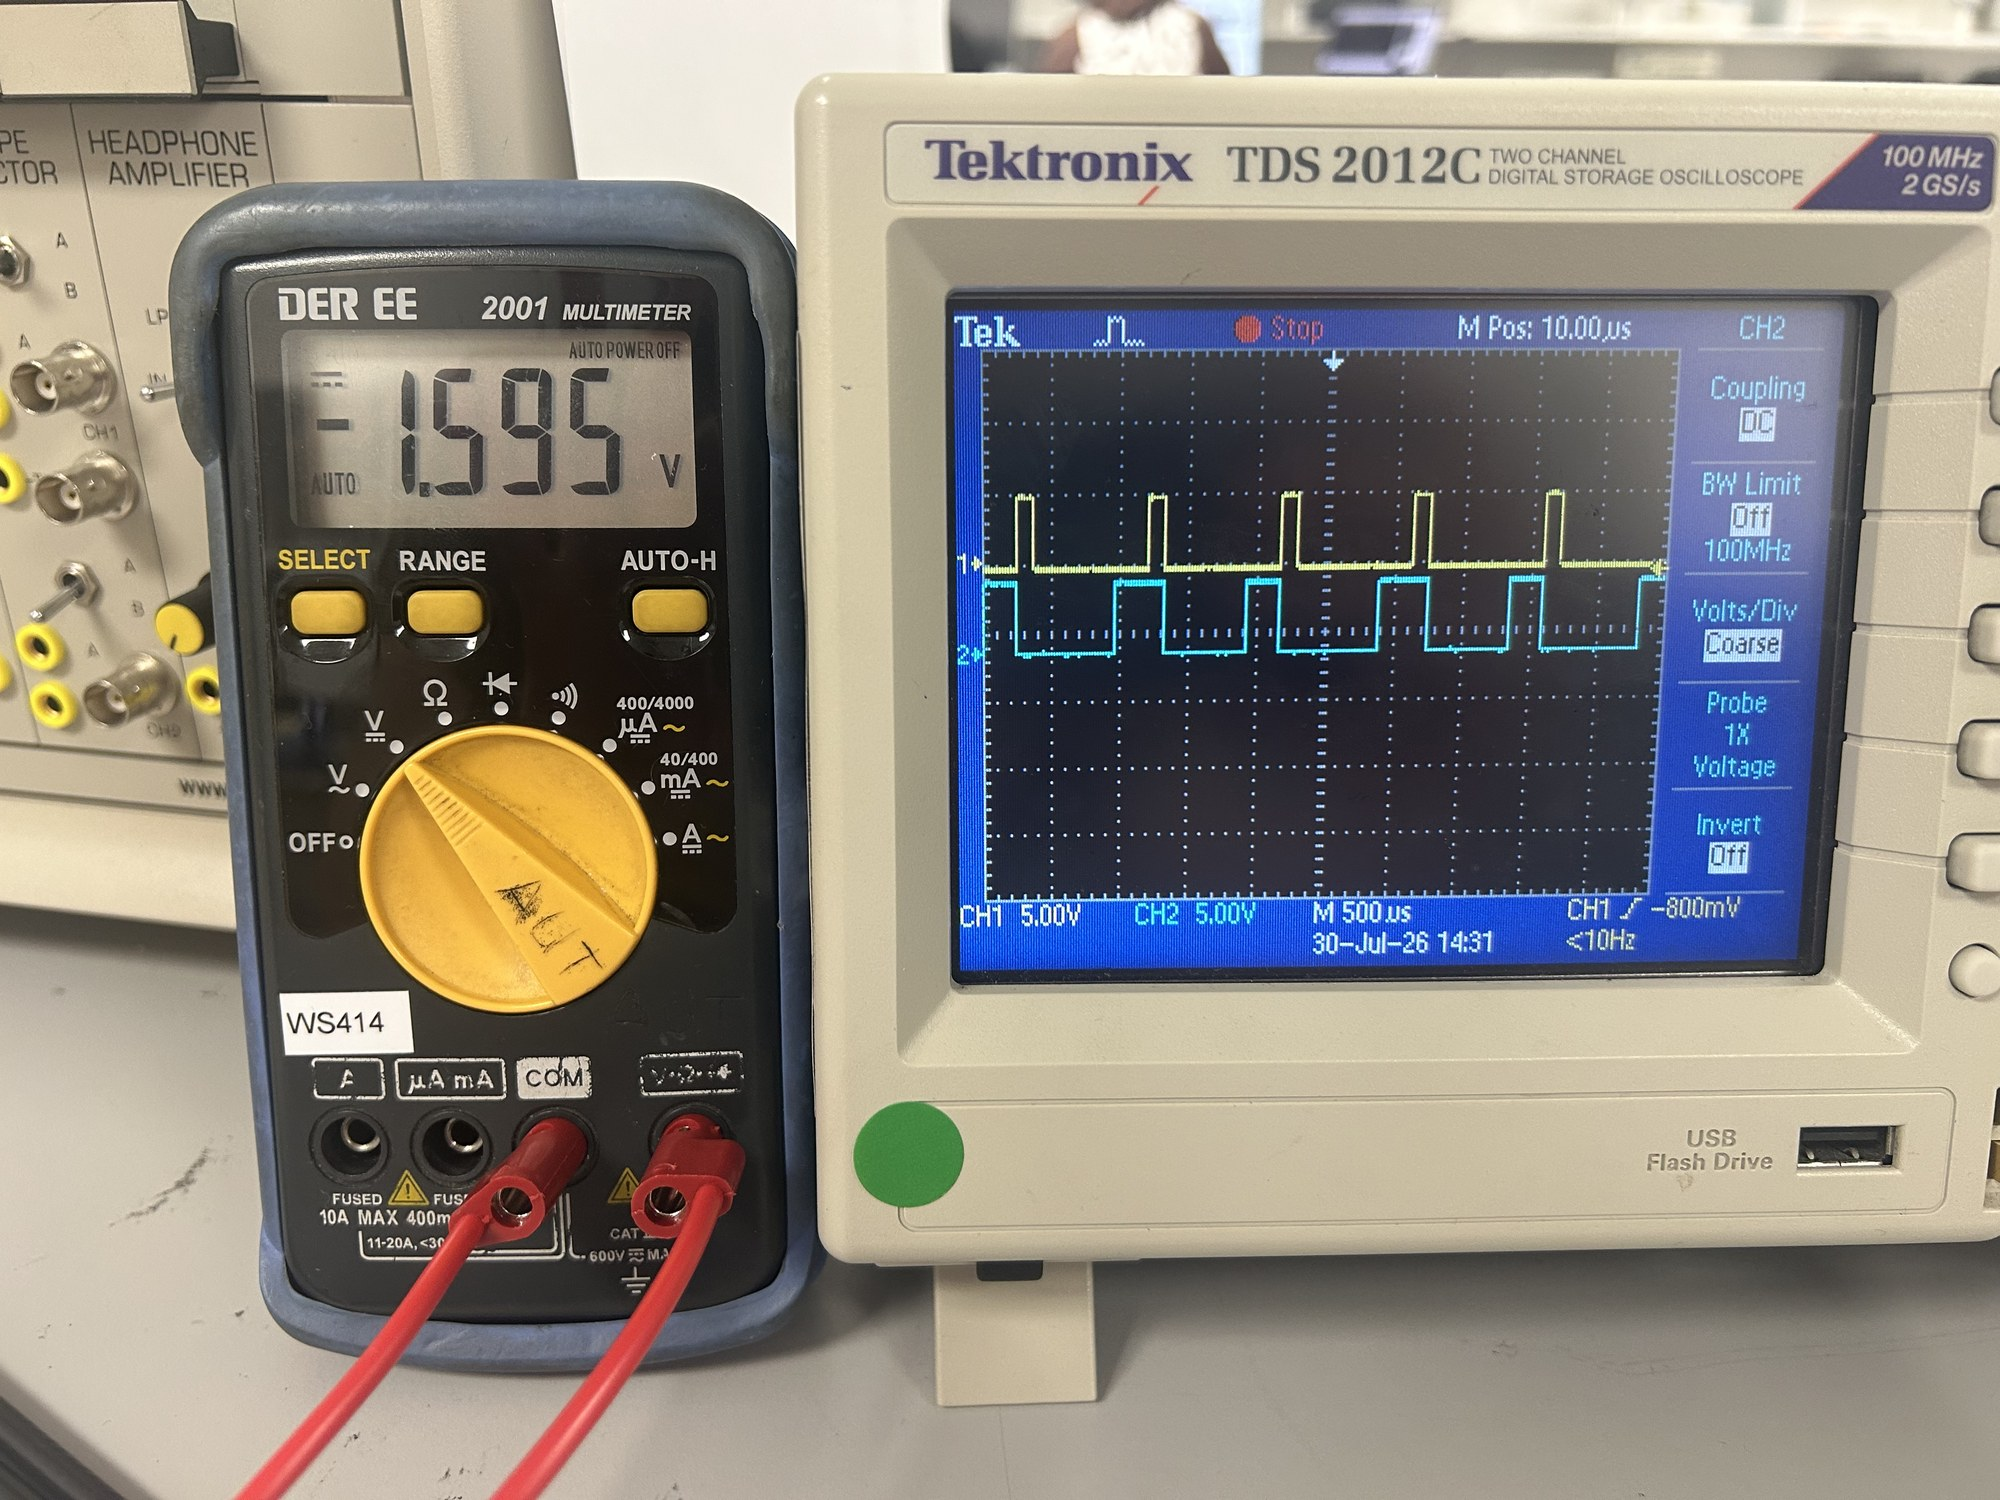
\includegraphics[width=\linewidth]{lab4_q41_minus1595.jpg}
  \caption{$-1.595$ V, code 0011.}
\end{subfigure}
\caption{Primary in-class photographic support for the first four Question 4.1 values. The meter signs and digits were checked directly at full resolution.}
\label{fig:q41-photos}
\end{figure}

\subsection{Question 4.2 partial companded data}

\begin{longtable}{r r c r}
\toprule
No. & $V_{in}$ (V) & Binary code & Decimal code \\
\midrule
\endhead
1 & $-2.632$ & 0000 & 0 \\
2 & $-1.100$ & 0001 & 1 \\
3 & $-0.522$ & 0010 & 2 \\
4 & $-0.291$ & 0011 & 3 \\
5 & $-0.154$ & 0100 & 4 \\
6 & $-0.003$ & 1001 & 9 \\
7 & $-0.072$ & 1011 & 11 \\
8 & $0.217$ & 1100 & 12 \\
9 & $0.308$ & 1101 & 13 \\
10 & $0.809$ & 1110 & 14 \\
11 & $1.272$ & 1111 & 15 \\
\bottomrule
\end{longtable}

\begin{figure}[H]
  \centering
  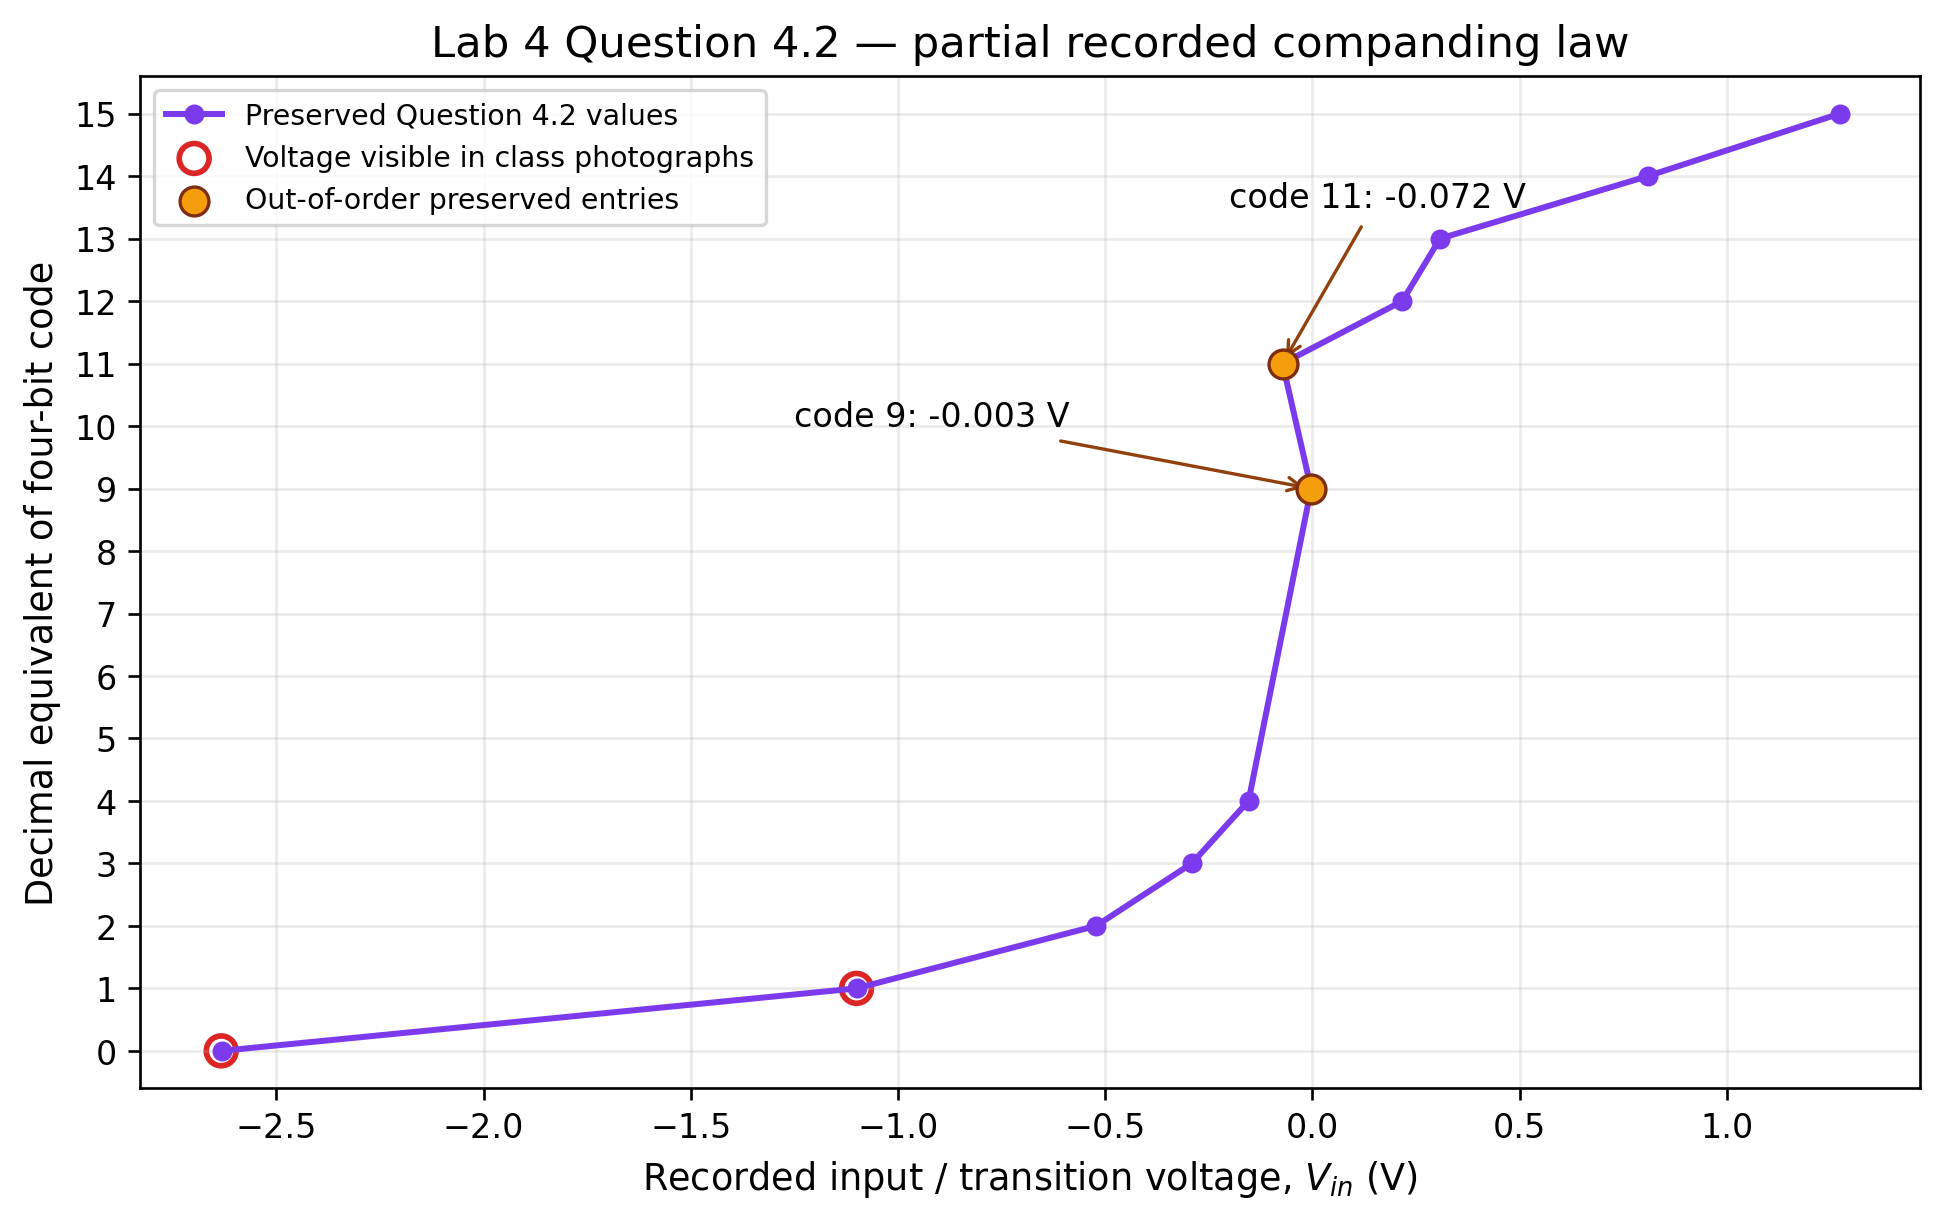
\includegraphics[width=0.96\textwidth]{lab4_q42_companding_partial.png}
  \caption{My graph of the partial Question 4.2 data. Missing codes create gaps, and the preserved code-9/code-11 pair is not monotonic. I show these limitations instead of interpolating invented measurements.}
  \label{fig:q42-compand}
\end{figure}

\begin{figure}[H]
\centering
\begin{subfigure}[t]{0.49\textwidth}
  \centering
  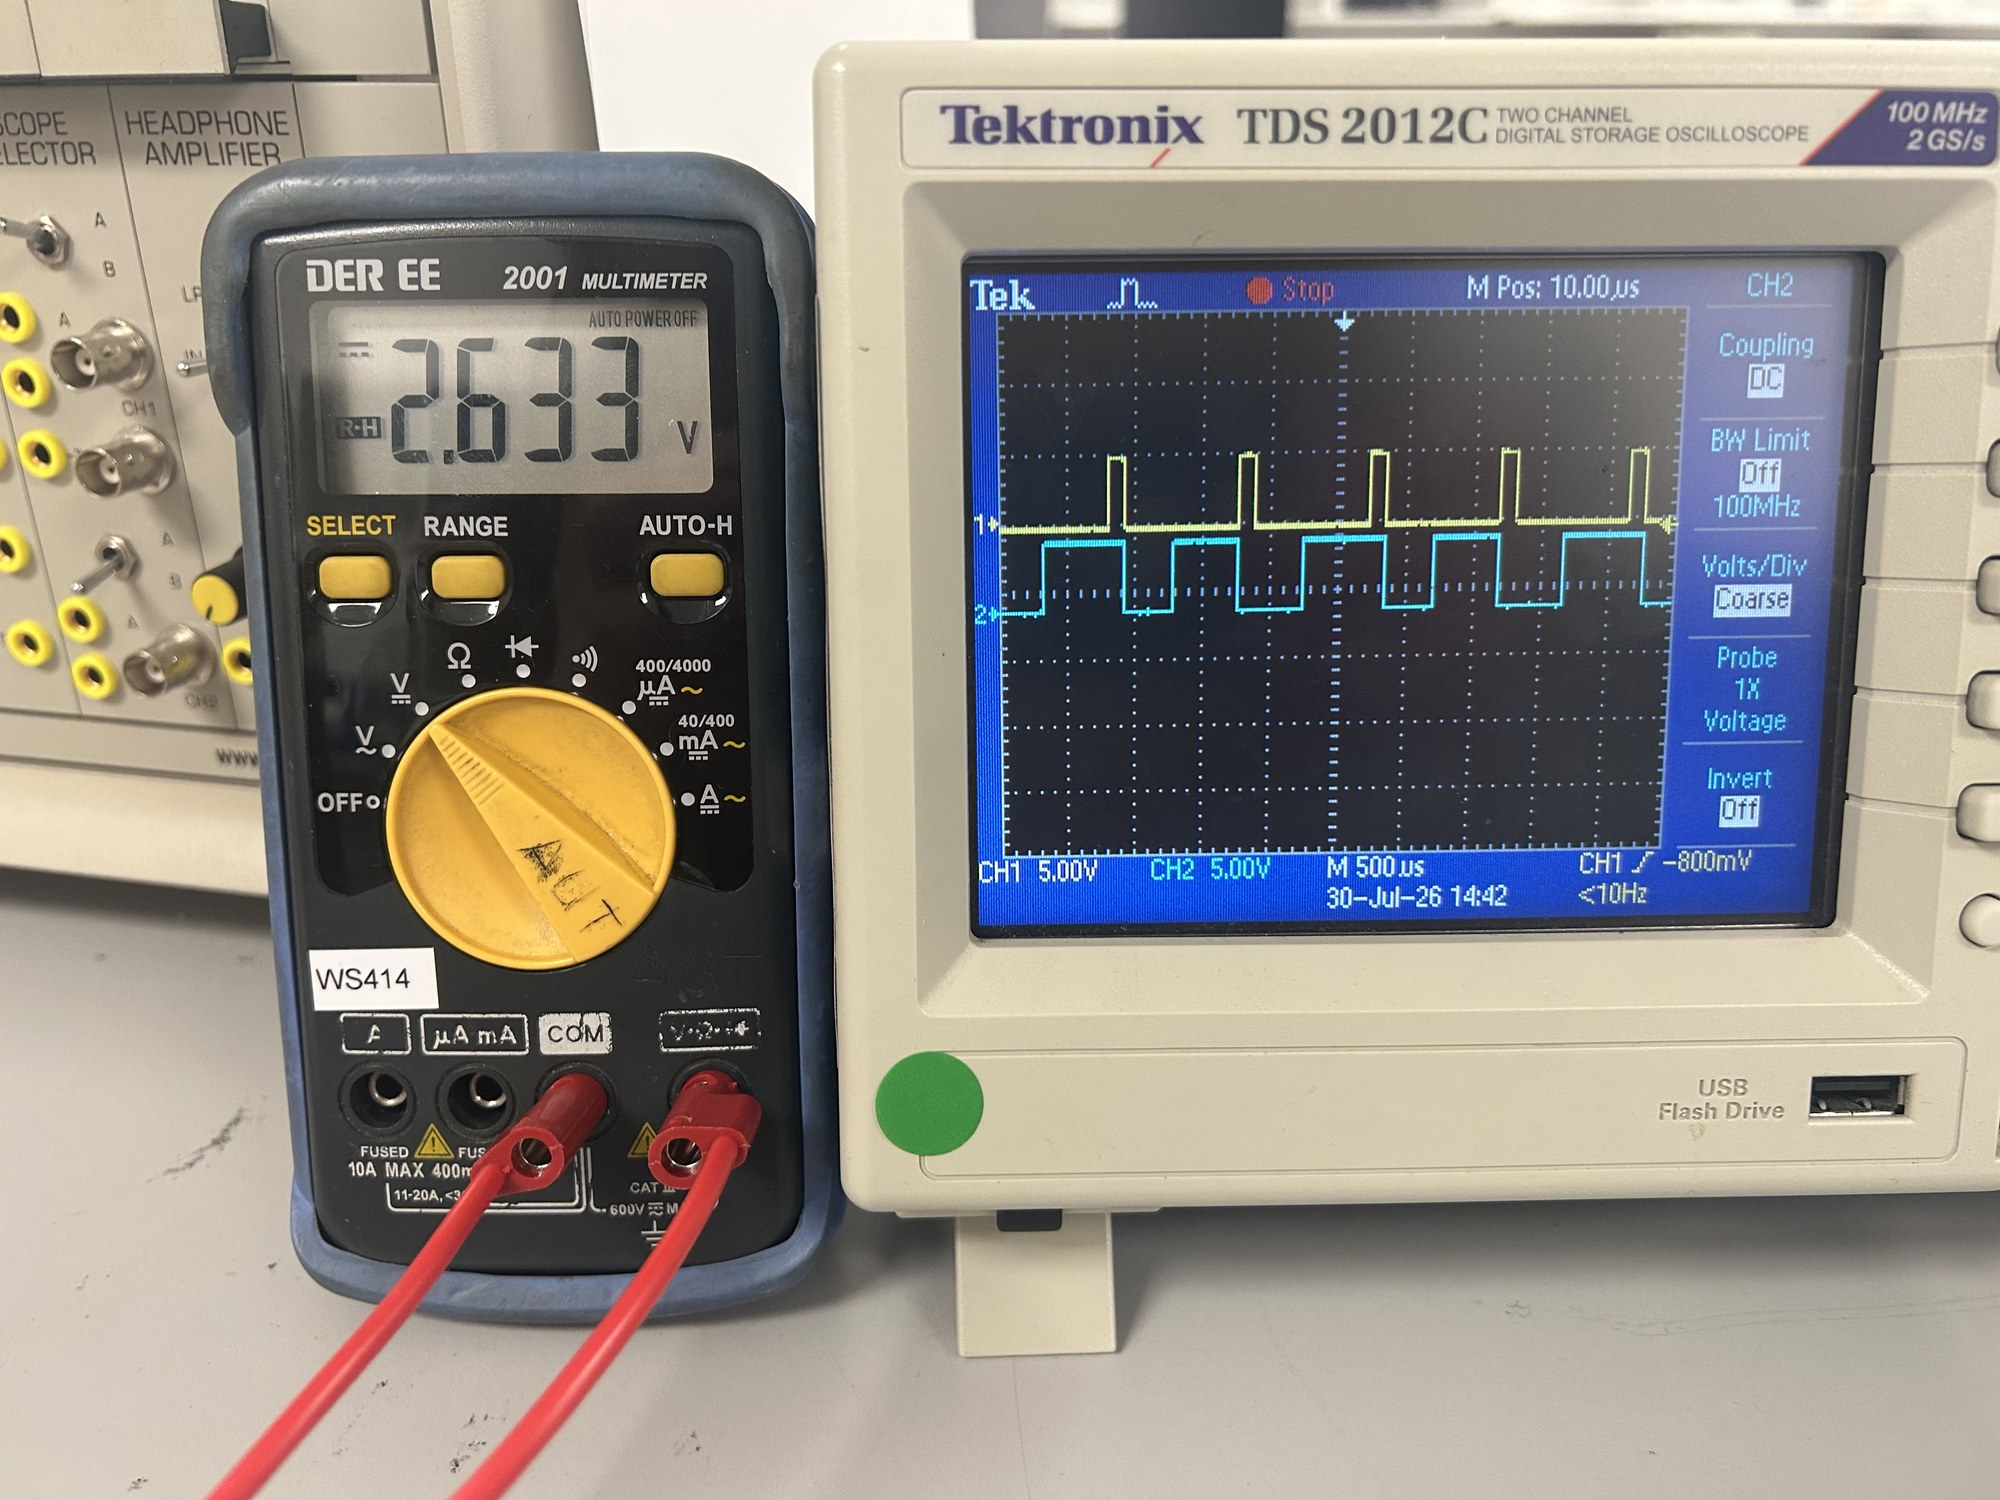
\includegraphics[width=\linewidth]{lab4_q42_minus2633.jpg}
  \caption{$-2.633$ V, matching code 0000.}
\end{subfigure}\hfill
\begin{subfigure}[t]{0.49\textwidth}
  \centering
  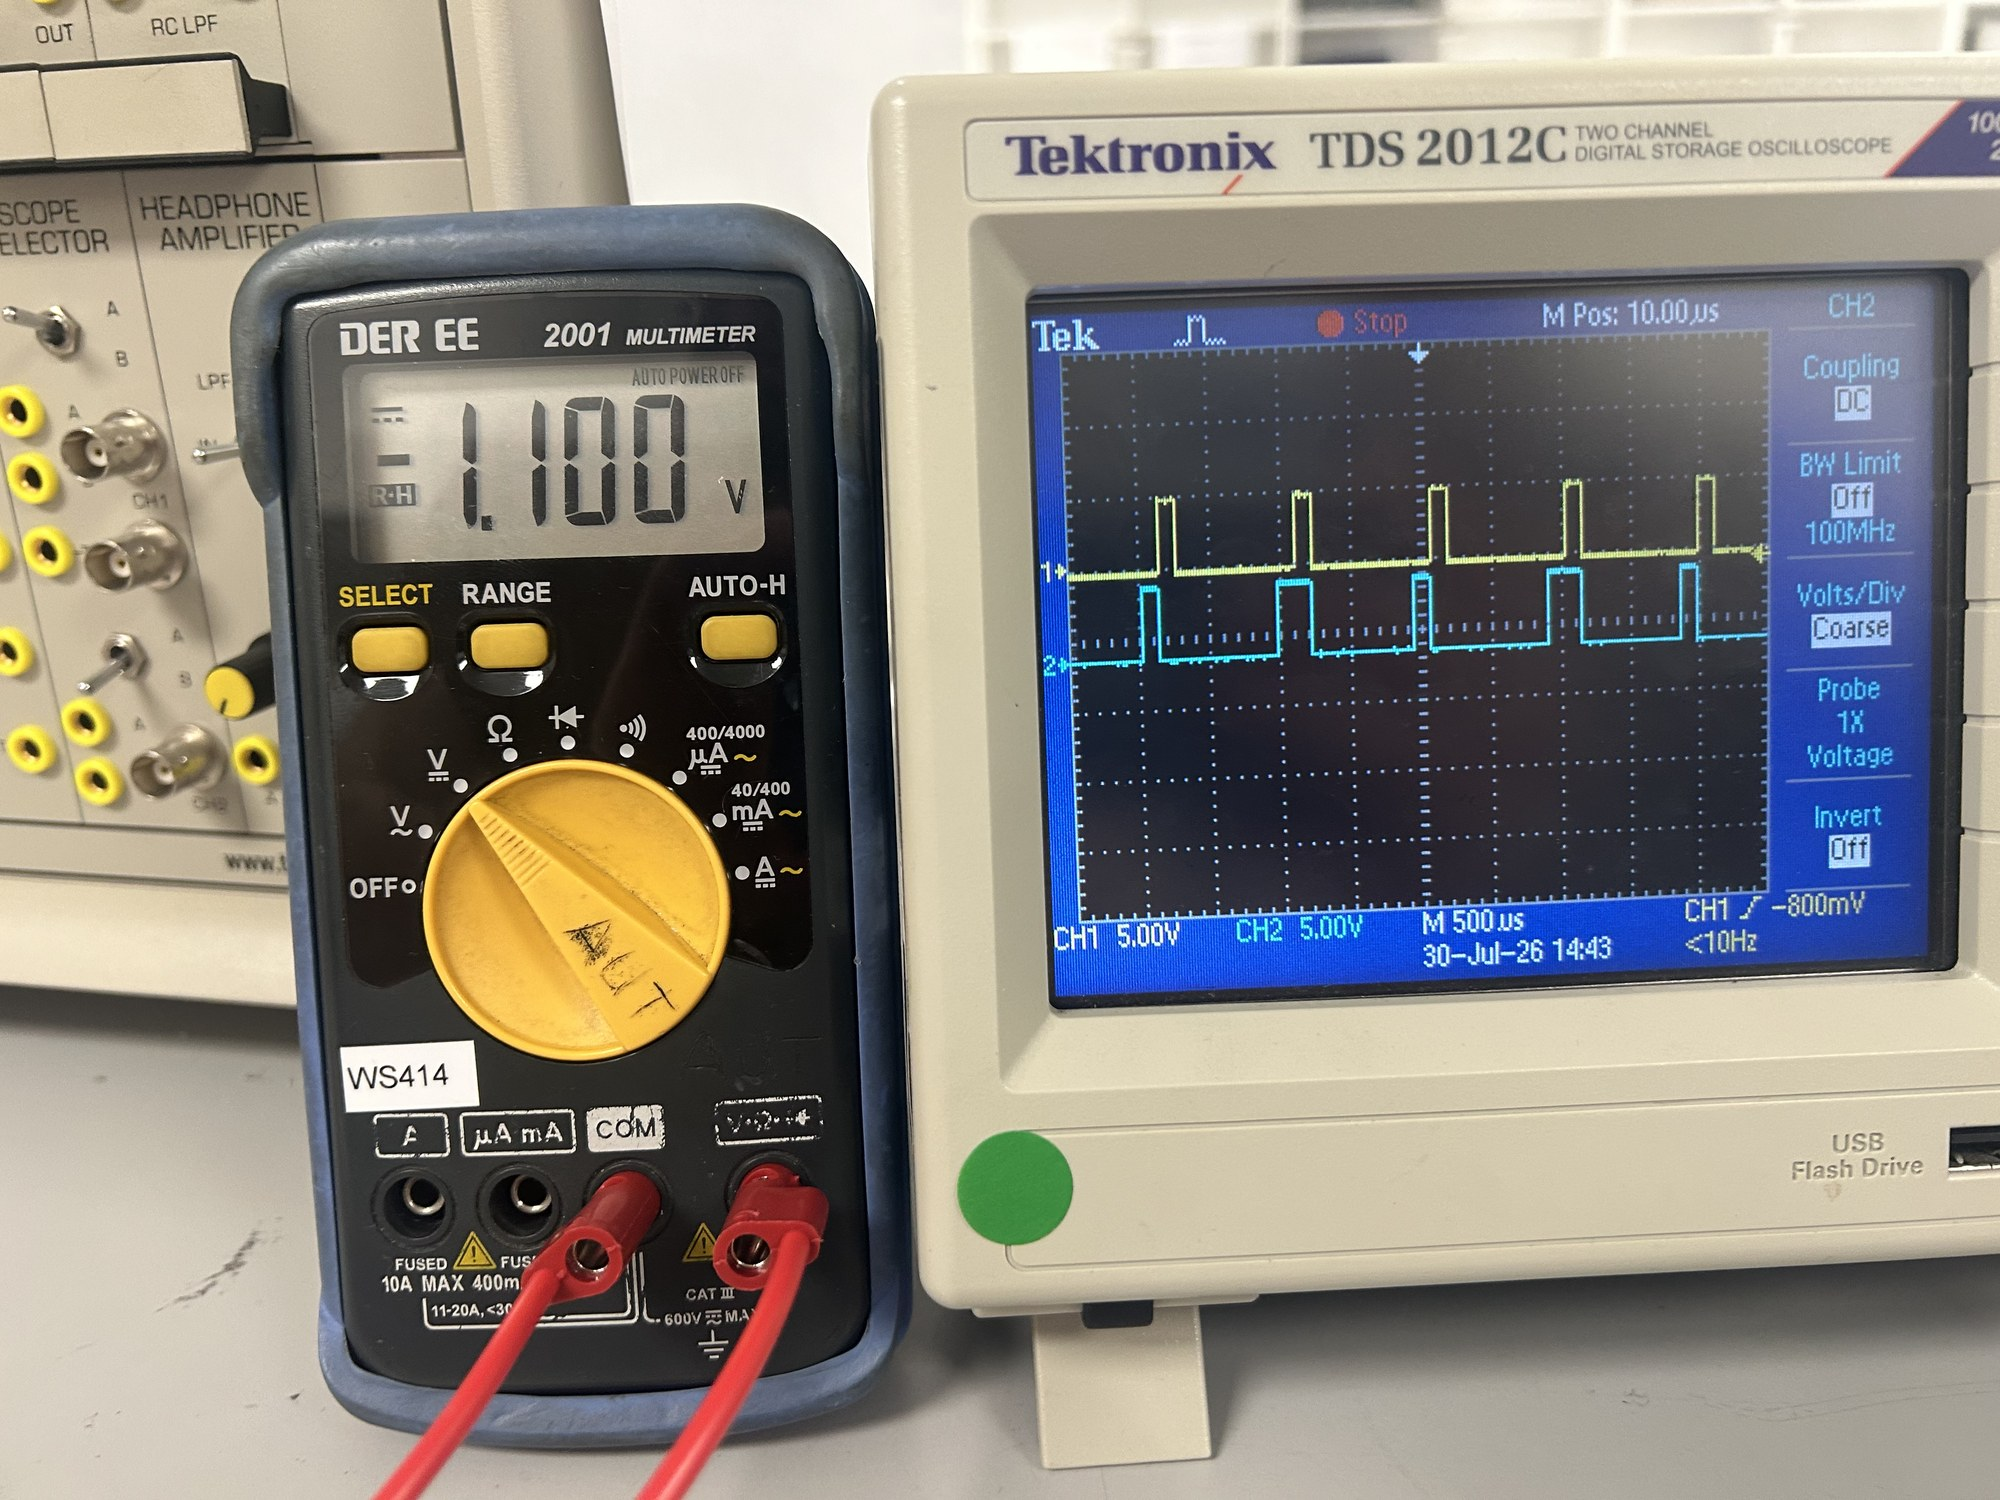
\includegraphics[width=\linewidth]{lab4_q42_minus1100.jpg}
  \caption{$-1.100$ V, matching code 0001.}
\end{subfigure}
\caption{Primary in-class photographic support for the first two Question 4.2 values.}
\label{fig:q42-photos}
\end{figure}

\begin{figure}[H]
  \centering
  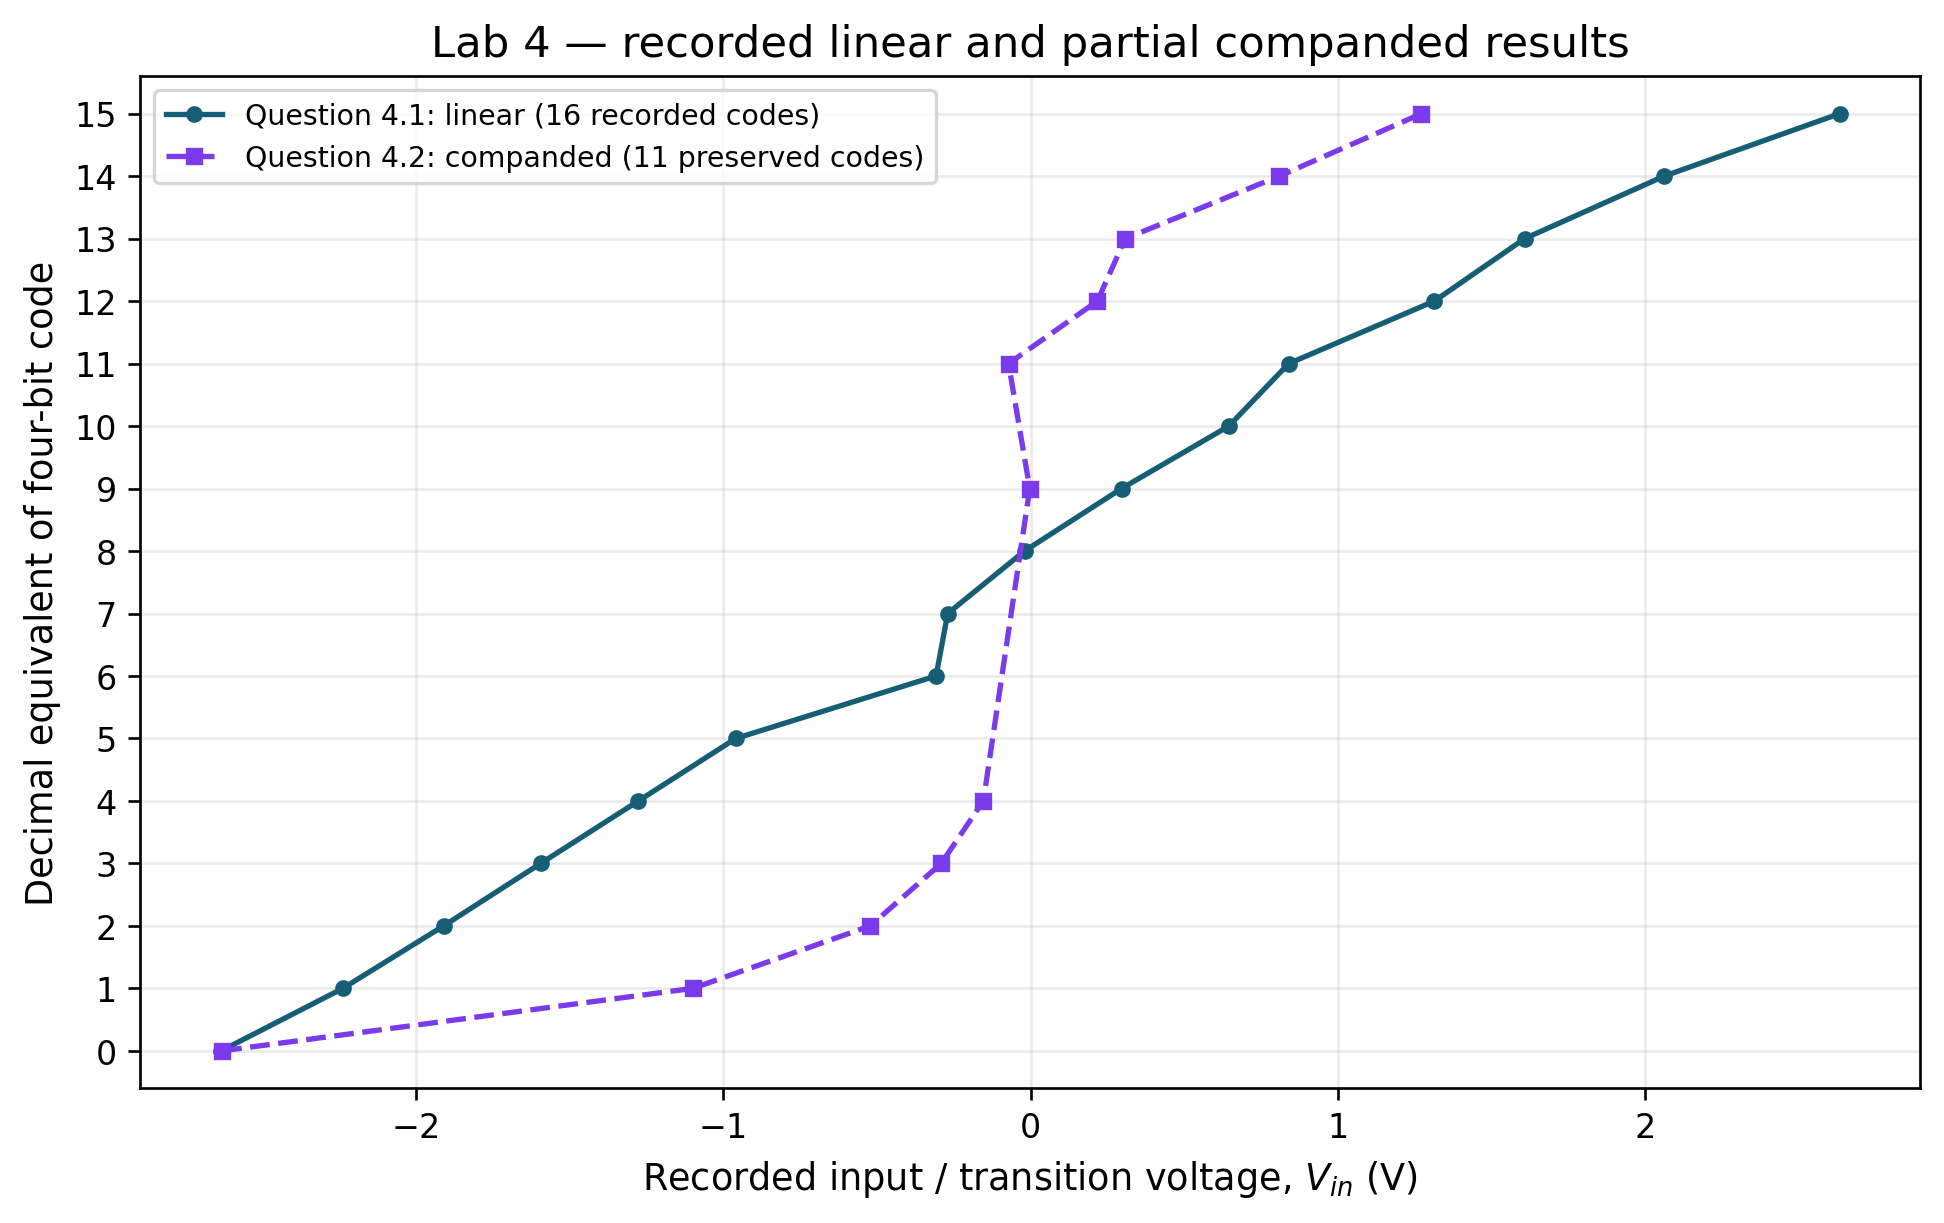
\includegraphics[width=0.96\textwidth]{lab4_linear_companded_comparison.png}
  \caption{Direct comparison of my complete raw linear sequence and the partial preserved companded sequence. This plot shows the expected non-uniform character qualitatively, but the incomplete and out-of-order companded record prevents a final quantitative companding-law fit.}
  \label{fig:comparison}
\end{figure}
\subsection{Second session: encoder/decoder continuation}
In the second Lab 4 session, Iyla, Amber, Nihil and I attended. Iyla read ahead while Nihil and I connected the encoder and decoder and continued data collection; Amber was present and supported the group. The complete 16-row encoder/decoder comparison showed close tracking across the code range.
\begin{figure}[H]\centering
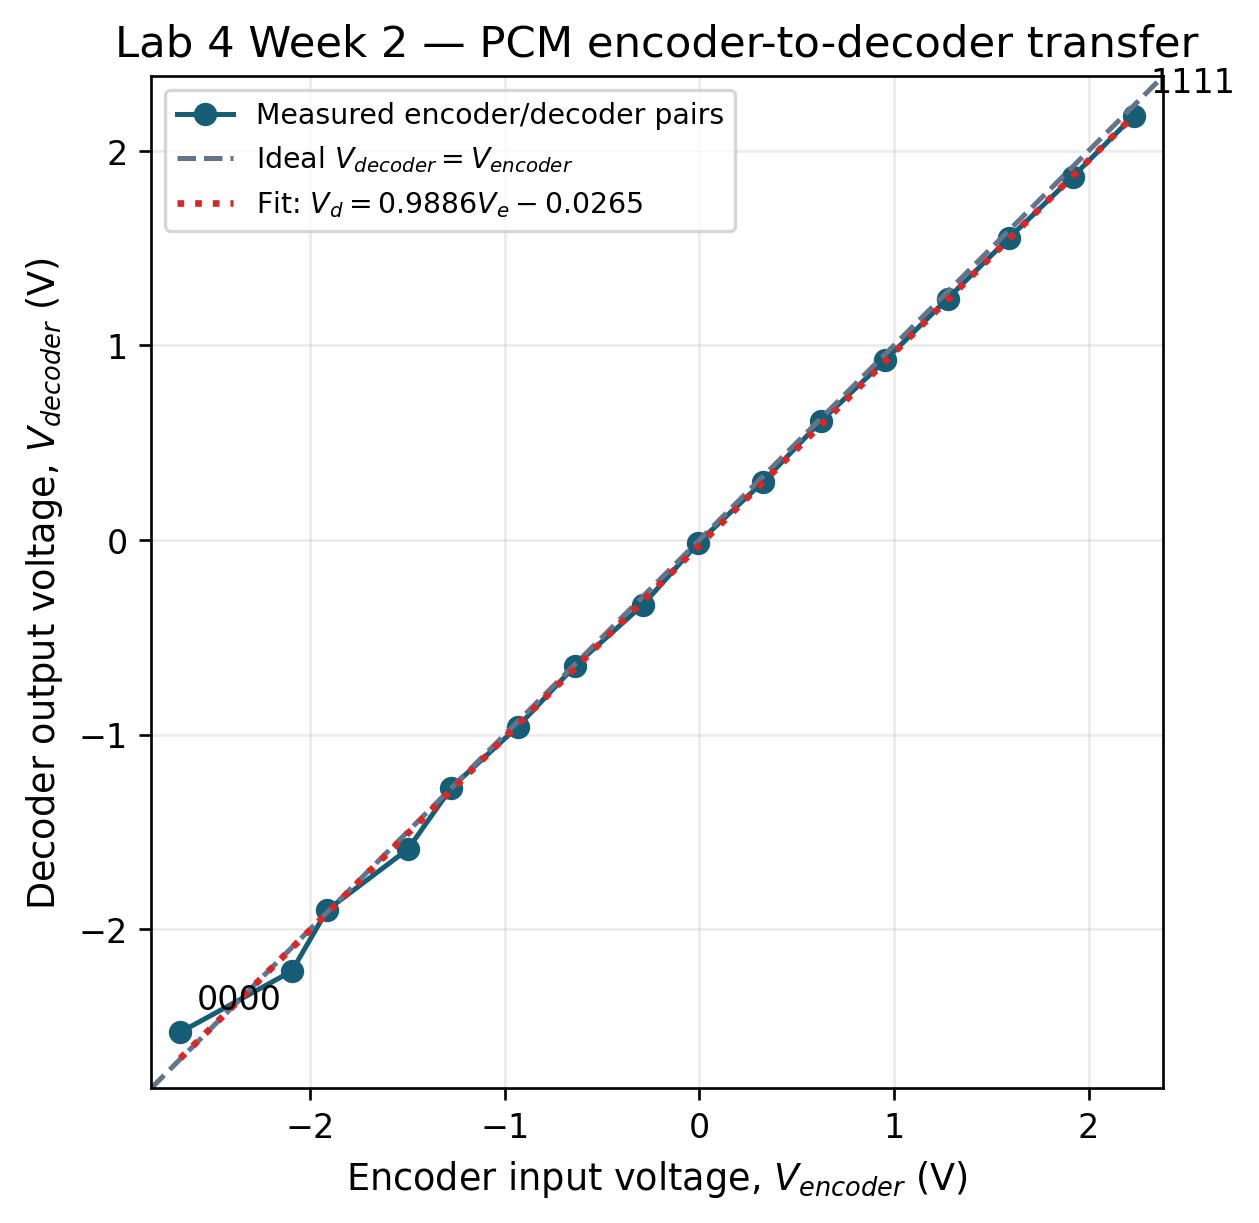
\includegraphics[width=0.95\textwidth]{lab4_week2_encoder_decoder_transfer.png}
\caption{Later verified graph of the second-session decoder output against encoder input. The fitted relationship was $V_{decoder}=0.9886V_{encoder}-0.0265$ V with $R^2=0.99879$.}
\end{figure}
\begin{figure}[H]\centering
\begin{subfigure}[t]{0.49\textwidth}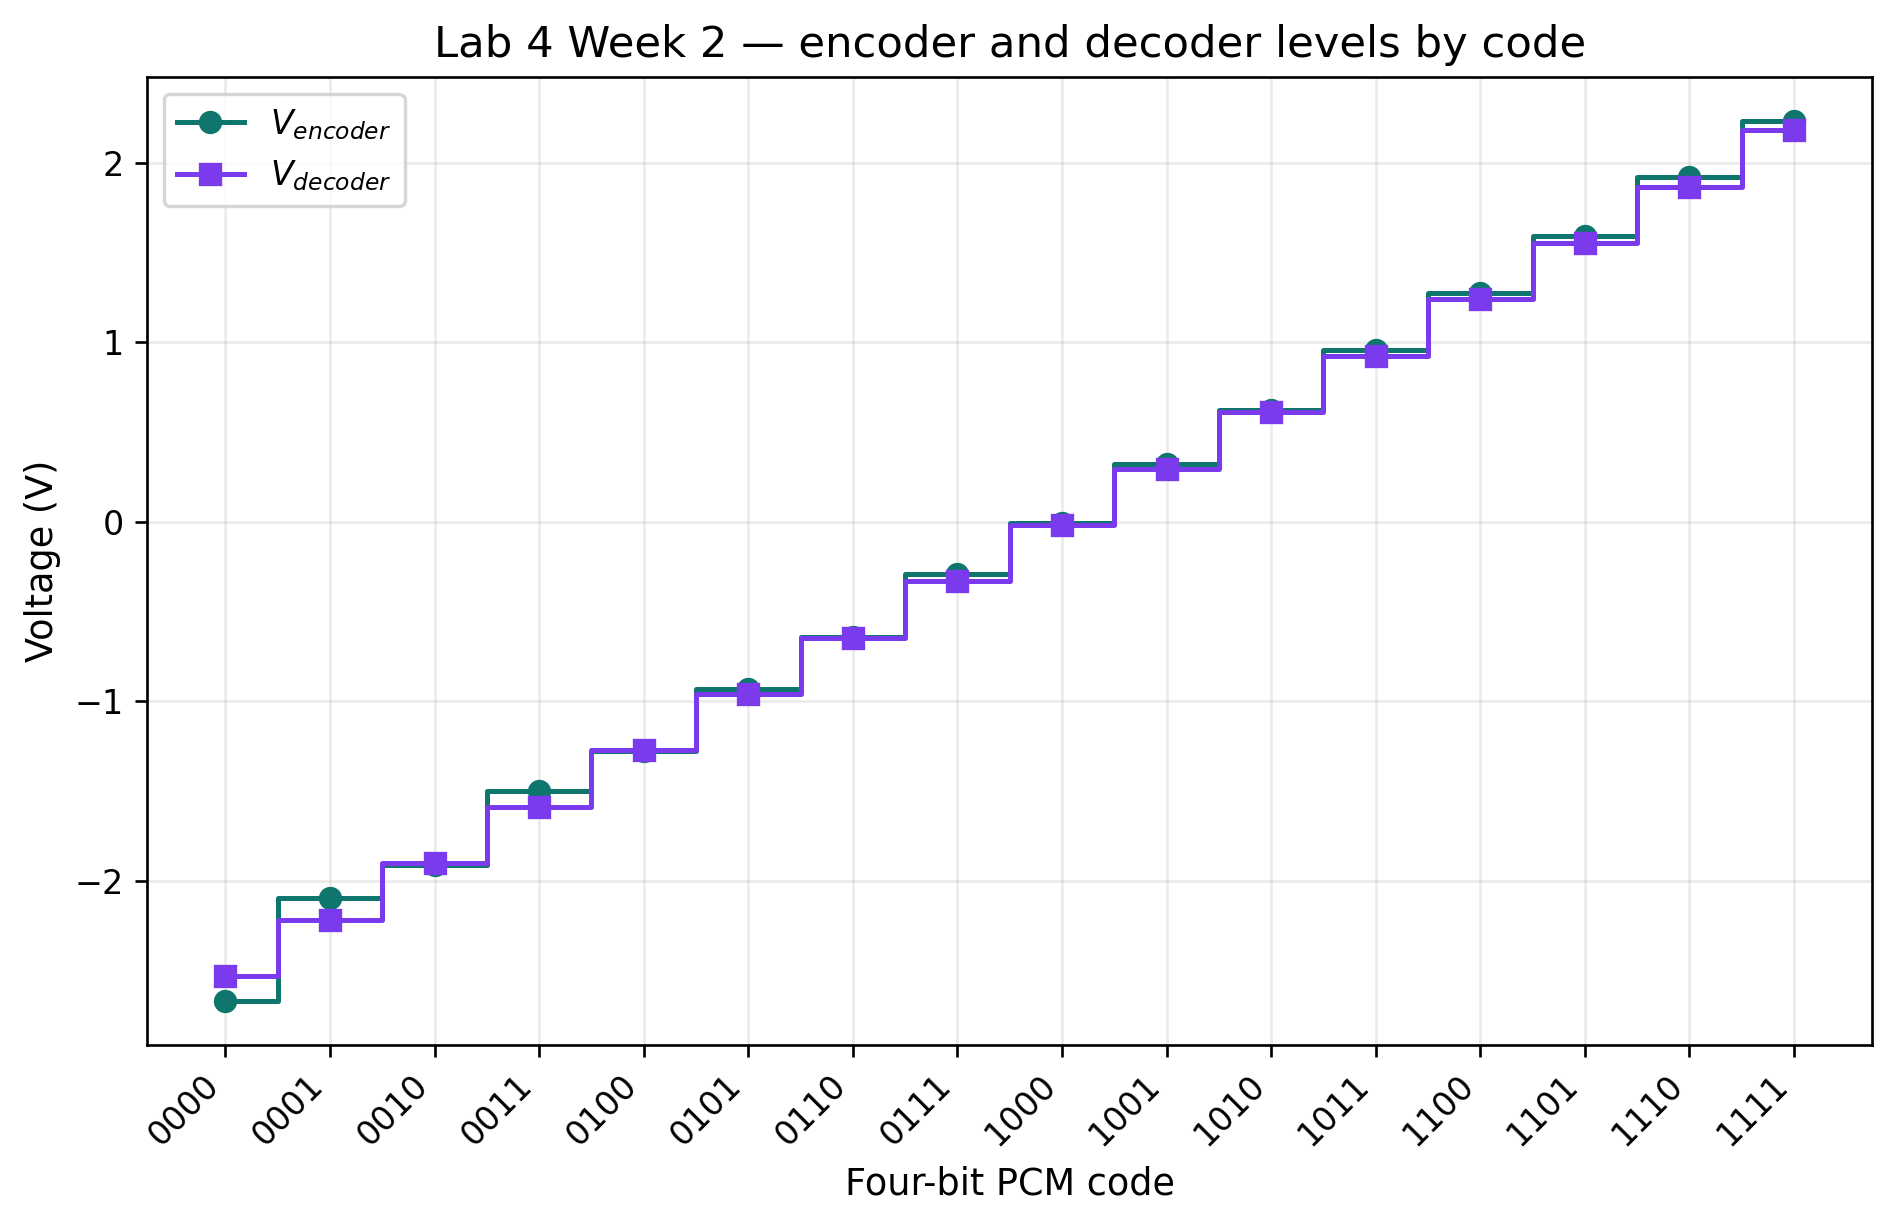
\includegraphics[width=\linewidth]{lab4_week2_levels_by_code.png}\caption{Encoder and decoder levels by code.}\end{subfigure}\hfill
\begin{subfigure}[t]{0.49\textwidth}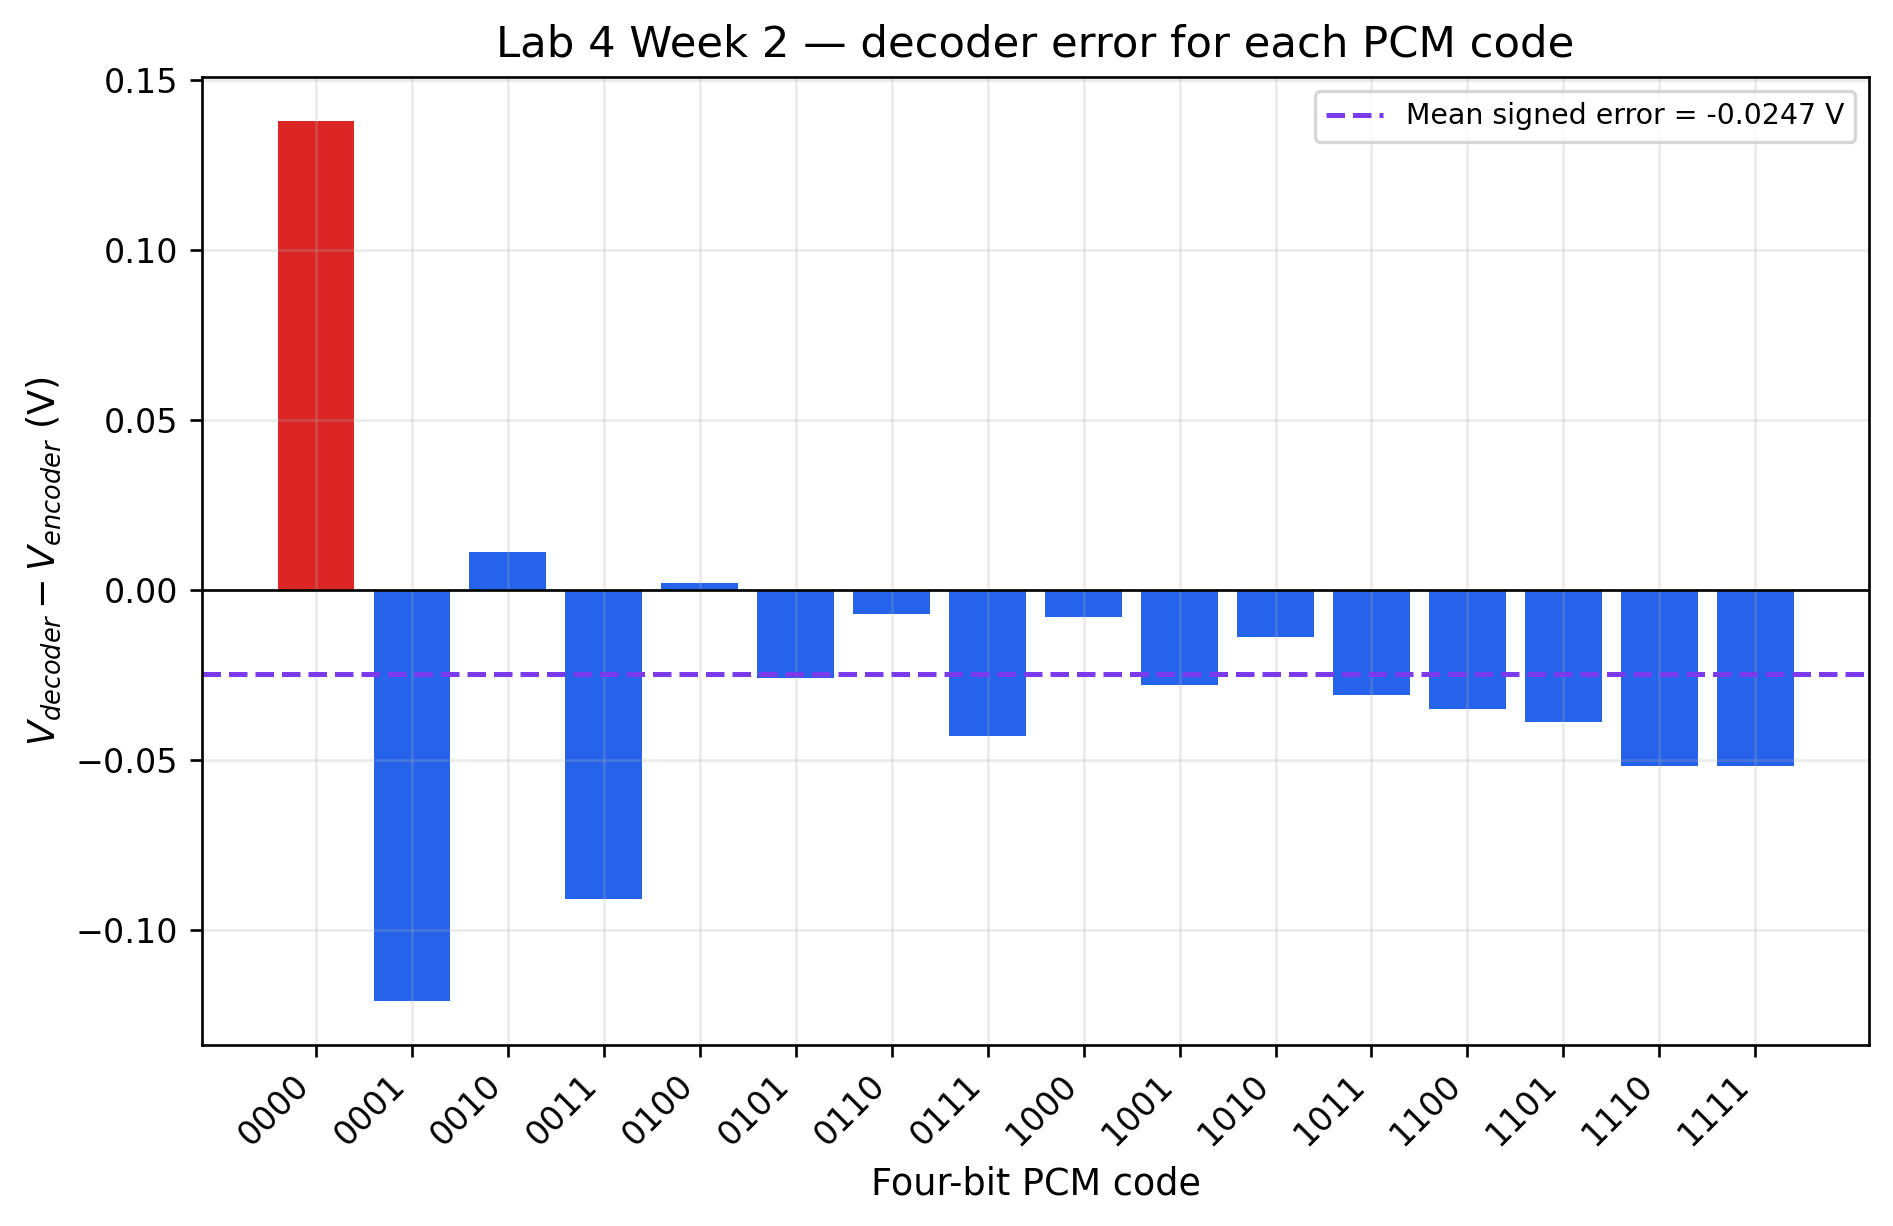
\includegraphics[width=\linewidth]{lab4_week2_decoder_error.png}\caption{Decoder-minus-encoder error by code.}\end{subfigure}
\caption{The mean absolute error was 0.0436 V, RMSE 0.0585 V, mean signed error $-0.0248$ V and maximum absolute error 0.138 V.}
\end{figure}

\subsection{Manual questions answered}
\subsection{Question 1: sampling rate and input bandwidth}
\begin{answerbox}
The master clock was $f_{CLK}=8.333$ kHz and one PCM frame occupied eight clock periods. I calculated
\[
 f_s=\frac{8333}{8}=1041.625\ \text{samples/s}.
\]
This is the same for 4-bit and 7-bit coding because the TIMS frame remains eight slots long in both modes; the selected mode changes the number of data slots used, not the frame rate. By the Nyquist criterion, the theoretical maximum input bandwidth is
\[
 B_{max}=\frac{f_s}{2}=520.8125\ \text{Hz}.
\]
In practice, I would keep the message below this boundary and use suitable anti-alias filtering.
\end{answerbox}

\subsection{Question 2: 4-bit timing and quantisation}
\begin{answerbox}
\begin{enumerate}[label=(\alph*)]
\item Sampling rate: $1041.625$ samples/s.
\item Frame width: $8/8333=0.960038$ ms.
\item Data-bit width: $1/8333=120.005$ $\mu$s.
\item Four-bit data-word width: $4/8333=480.019$ $\mu$s.
\item Number of quantising levels: $2^4=16$.
\item The ideal 4-bit linear mode should have uniformly spaced levels. My raw graph is broadly increasing and covers all 16 codes, but the transcribed central values make the measured spacing non-uniform. I cannot honestly claim close uniformity until those entries are checked.
\end{enumerate}
\end{answerbox}

\subsection{Question 3: definition and composition of a frame}
\begin{answerbox}
I define a frame as the eight-clock-slot interval used to carry the encoded value of one analogue sample together with synchronisation information. In 4-bit mode, slots 7--5 remain zero, slots 4--1 carry the four-bit data word, and slot 0 carries the encoder's alternating embedded frame-synchronisation bit.

\begin{center}
\begin{tabular}{c|c|c|c|c|c|c|c|c}
\toprule
Slot & 7 & 6 & 5 & 4 & 3 & 2 & 1 & 0 \\
\midrule
Content & 0 & 0 & 0 & $D_3$ & $D_2$ & $D_1$ & $D_0$ & FS \\
\bottomrule
\end{tabular}
\end{center}
The FS bit alternates 1, 0, 1, 0 across successive frames. At 8.333 kHz, equal-valued embedded pulses recur every two frames, approximately $1.920$ ms apart.
\end{answerbox}

\subsection{Question 4: transmitting frames more slowly}
\begin{answerbox}
I could store completed frames in a buffer or memory, then transmit the stored bits using a slower serial clock and reconstruct their original timing at the receiver using a buffer, recovered clock and frame synchronisation. This introduces delay and requires enough storage. A continuously operating source cannot be sent forever at an average information rate below the rate at which bits are produced unless I also reduce, compress or discard information. Slower delayed transmission is useful for recorded data, burst transmission, time-division sharing, or a channel whose instantaneous rate is low but where delay is acceptable.
\end{answerbox}

\subsection{Question 5: stable and unstable oscilloscope displays}
\begin{answerbox}
A DC message is constant, so every sample is assigned the same quantisation code. Triggering on frame synchronisation overlays identical PCM frames and gives a stable display. With a sinusoidal message, the sample amplitude changes from frame to frame, so the encoder produces different code words. When those frames are repeatedly overlaid, the PCM data appears unstable or as many superimposed patterns unless I capture a single frame or synchronise over the complete repeating message sequence.
\end{answerbox}

\subsection{Question 6: quantisation diagram and experimental method}
\begin{answerbox}
Figure~\ref{fig:q41-linear} is my measured quantisation diagram. I started near the maximum negative input, read the four data bits in slots 4--1, converted each binary word to decimal, and slowly increased the Variable DC input. Each time the PCM word changed, Nahil and I recorded the meter voltage and the new code. We continued until the sequence reached 1111. The photograph series in Figure~\ref{fig:q41-photos} directly supports the first four measured code regions.
\end{answerbox}

\subsection{Question 7: reconstruction-filter amplitude characteristic}
\begin{answerbox}
I would require a low-pass filter with a substantially flat amplitude response across the wanted message band and strong attenuation at the sampling images above that band. If I am using the output to measure second- and third-order message harmonics, the passband must extend far enough to retain those harmonics; otherwise the filter would hide distortion and give a falsely optimistic result. Passband ripple should be small enough that it does not materially change the measured message amplitudes.
\end{answerbox}

\subsection{Question 8: reconstruction-filter specification}
\begin{answerbox}
I would start with the maximum wanted message frequency, the $1041.625$ samples/s sampling rate, and the location of the first spectral image. I would then specify: passband edge; acceptable passband ripple; stopband edge and attenuation; transition width; allowable phase or group-delay distortion; load and signal levels; and whether the second and third message harmonics must remain measurable. The final cutoff must pass the wanted content while rejecting the high-frequency sample-and-hold components as much as the available transition band allows.
\end{answerbox}

\subsection{Question 9: reducing sampling and quantisation distortion}
\begin{answerbox}
For sampling distortion from a sample-and-hold system, I can raise the sampling rate relative to the message bandwidth, use appropriate anti-alias and reconstruction filters, and compensate sample-and-hold aperture droop where necessary. For quantisation distortion, I can increase the number of bits and levels, scale the signal so it uses the available input range without clipping, or use a suitable non-uniform quantiser/compander for signals such as speech.
\end{answerbox}

\subsection{Question 10: cost of increasing the number of levels}
\begin{answerbox}
More quantisation levels require more bits per sample. The price is greater converter and decoder complexity, a higher serial bit rate or more occupied frame slots, more storage, wider channel bandwidth when the sample rate is unchanged, and potentially greater power and clocking demands. In this TIMS experiment, the cost was visible as extra data-bit positions: 7-bit mode uses seven data slots instead of four. Because the frame was fixed at eight clock periods, the sample rate itself remained unchanged, but the resolution and number of occupied data slots increased.
\end{answerbox}
\weeklynote{\textbf{Week 3:} Nahil and I learned how to align and read the four PCM data slots, then divided adjustment and recording roles.\\\textbf{Week 4:} Iyla, Amber, Nihil and I continued with encoder/decoder patching, complete data collection, reconstruction and FFT inspection.\\\textbf{Main lesson:} Draw and label the whole signal path before patching, verify one signal at a time, and write scope settings beside each photo.}
\labdivider
\section{Lab 5 -- Amplitude Modulation using Simulink}
\subsection{Open labbook questions}
\subsubsection*{What exact code or plotting change produced the three stacked spectra?}
\begin{answerbox}
The preserved files do not identify one decisive line as the final fix. What I can verify is the final working arrangement: I selected each axis with \texttt{subplot(3,1,k)} before calling \texttt{sigspec} for the modulating signal, carrier and modulated signal. I also had to keep the signals in compatible vector orientations and use the same spectrum function for all three. This produced three separate, vertically stacked spectra rather than repeatedly drawing into one axis. I should not claim a more specific last edit because I did not record it at the time.
\end{answerbox}

\subsubsection*{Did a lecturer or classmate identify the decisive fix?}
\begin{answerbox}
I did not preserve enough evidence to attribute the decisive plotting fix to a lecturer or classmate. My logbook records collaborative troubleshooting and several attempts, but it does not name a person who supplied the final correction. I therefore leave the attribution unclaimed.
\end{answerbox}

\subsubsection*{What did the final Scope show?}
\begin{answerbox}
Our saved model routed the Product output to a Scope, so the intended Scope result was an AM double-sideband suppressed-carrier waveform: a rapidly oscillating carrier whose positive and negative envelope followed the two-arch message. However, I did not preserve an identifiable in-class Scope capture. The strongest saved class result is the final three-spectrum screenshot below. I therefore use the Scope description as the expected interpretation of the model, not as a claim about a missing screenshot.
\end{answerbox}

\begin{figure}[H]
  \centering
  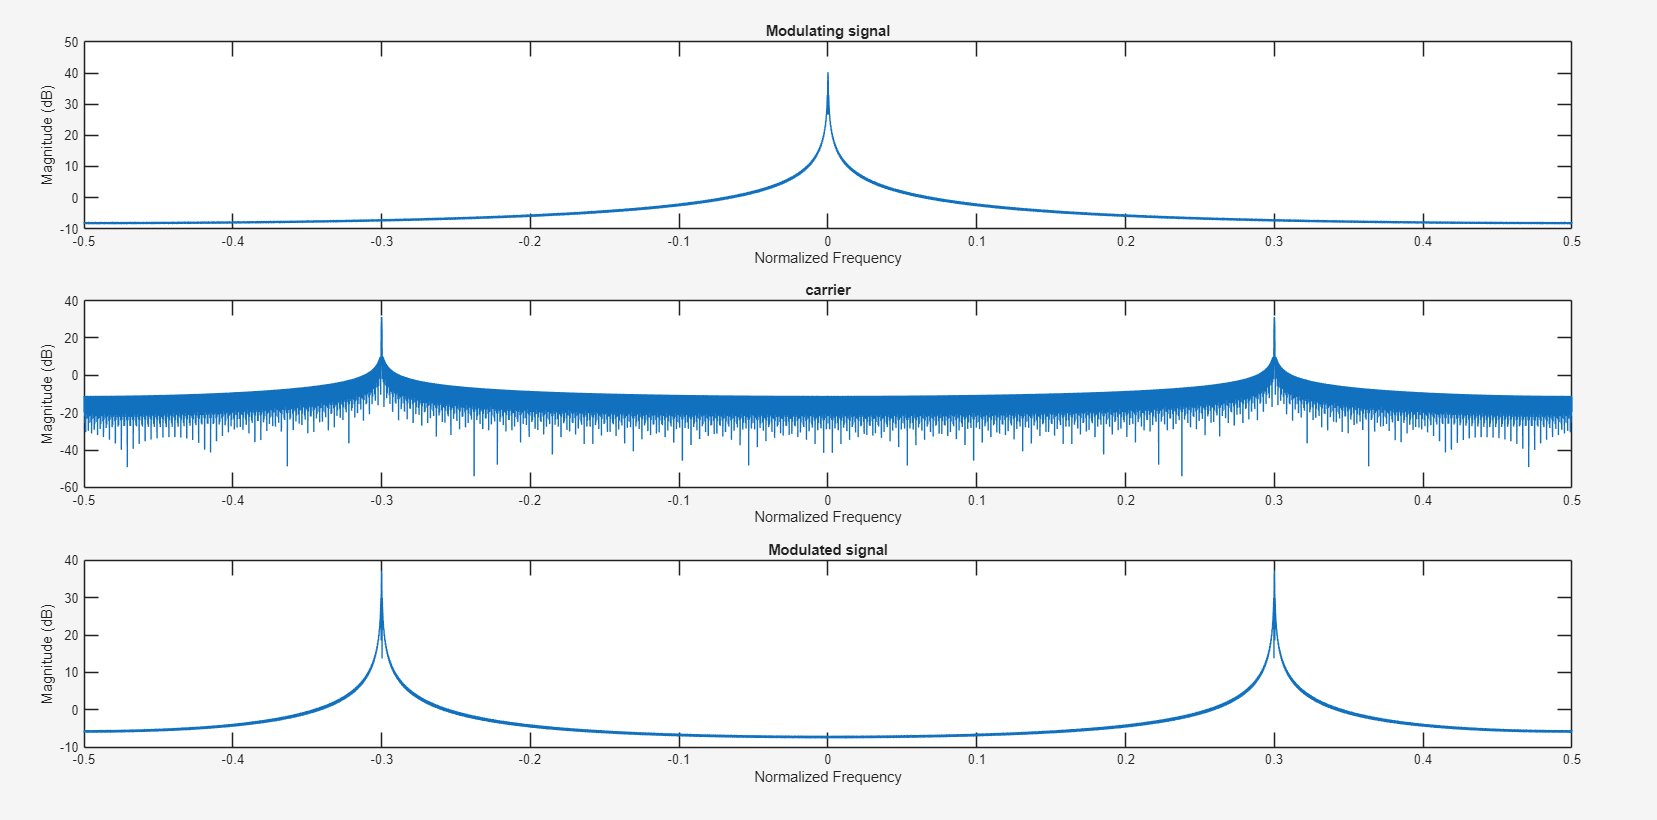
\includegraphics[width=0.96\textwidth]{lab5_inclass_spectra.png}
  \caption{Primary in-class evidence from Lab 5: our saved three-spectrum result. The baseband message is centred near zero, while the modulated spectrum is translated to the carrier regions near normalized frequency $\pm 0.3$.}
  \label{fig:lab5-class-spectra}
\end{figure}

\begin{figure}[H]
  \centering
  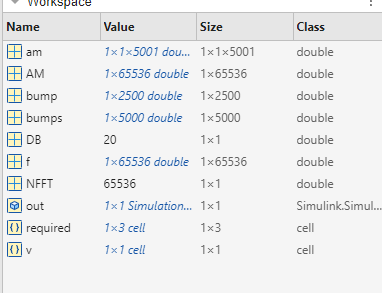
\includegraphics[width=0.48\textwidth]{lab5_workspace.png}
  \caption{Primary in-class MATLAB workspace evidence retained with our Lab 5 files.}
  \label{fig:lab5-workspace}
\end{figure}
\subsection{Manual questions answered}
\subsection{Question 1: MATLAB spectrum function}
\begin{answerbox}
I completed the supplied \texttt{sigspec} structure by forcing row inputs into columns, applying a Hamming window, using a zero-padded FFT, centring the spectrum with \texttt{fftshift}, and plotting either linear magnitude or the manual's $10\log_{10}$ magnitude. The function I used for the completed written answer is listed below. The optional outputs let me verify the peak locations numerically; they do not change the required plotting behaviour.
\end{answerbox}

\begin{lstlisting}[style=matlab,caption={My completed Lab 5 \texttt{sigspec.m} function.}]
function [f, siginspec] = sigspec(sigin, flag)
%SIGSPEC Display a signal spectrum using the ENEL700 Lab 5 method.
% Optional outputs are retained only for numerical verification.
if(nargin==0)
    disp('USAGE: sigspec(sigin,flag)');
    disp('   The input signals should be in the columns of sigin.');
    disp('   flag=0 produces a linear magnitude plot (default)');
    disp('   flag=1 produces a log magnitude plot (dB)');
    f = [];
    siginspec = [];
    return;
end
if(nargin==1)
    flag = 0;
end
[len,numsigs]=size(sigin);
if(len<numsigs)
    sigin = sigin.';
    tmp = len;
    len = numsigs;
    numsigs = tmp;
end
fftsize = 2^(ceil(log2(len))+2);
f=[0:fftsize-1].'/fftsize - 0.5;
sigin = repmat(hamming(len),1,numsigs).*sigin;
siginspec = abs(fftshift(fft(sigin,fftsize),1));
if(flag)
    plot(f,10*log10(siginspec));
    ylabel('Magnitude (dB)');
else
    plot(f,siginspec);
    ylabel('Linear magnitude');
end
xlabel('Normalized Frequency');
end
\end{lstlisting}

\subsection{Question 2: explanation of the three spectra and scaling}
\begin{answerbox}
In the first plot, the modulating signal is a baseband signal, so most of its spectral energy is centred near normalized frequency zero. In the second plot, the sinusoidal carrier gives narrow symmetric components at approximately $-0.3$ and $+0.3$. In the third plot, multiplying the message by the carrier shifts copies of the message spectrum from baseband to regions around $-0.3$ and $+0.3$. Because this is suppressed-carrier modulation, I do not expect a separate dominant unmodulated carrier line in the output.

For a unit cosine carrier,
\[
\cos(2\pi f_c n)=\tfrac{1}{2}e^{j2\pi f_c n}+\tfrac{1}{2}e^{-j2\pi f_c n},
\]
so each shifted copy has one-half of the original message-spectrum magnitude. My later numerical check measured a ratio of $0.498366$, close to the expected $0.5$. Under the manual's $10\log_{10}$ convention, this was $-3.0245$ dB, close to the expected $-3.0103$ dB. Figure~\ref{fig:lab5-class-spectra} remains the primary in-class plot; Figure~\ref{fig:lab5-scaling} is a later calculation used to verify the expected scaling.
\end{answerbox}

\begin{figure}[H]
  \centering
  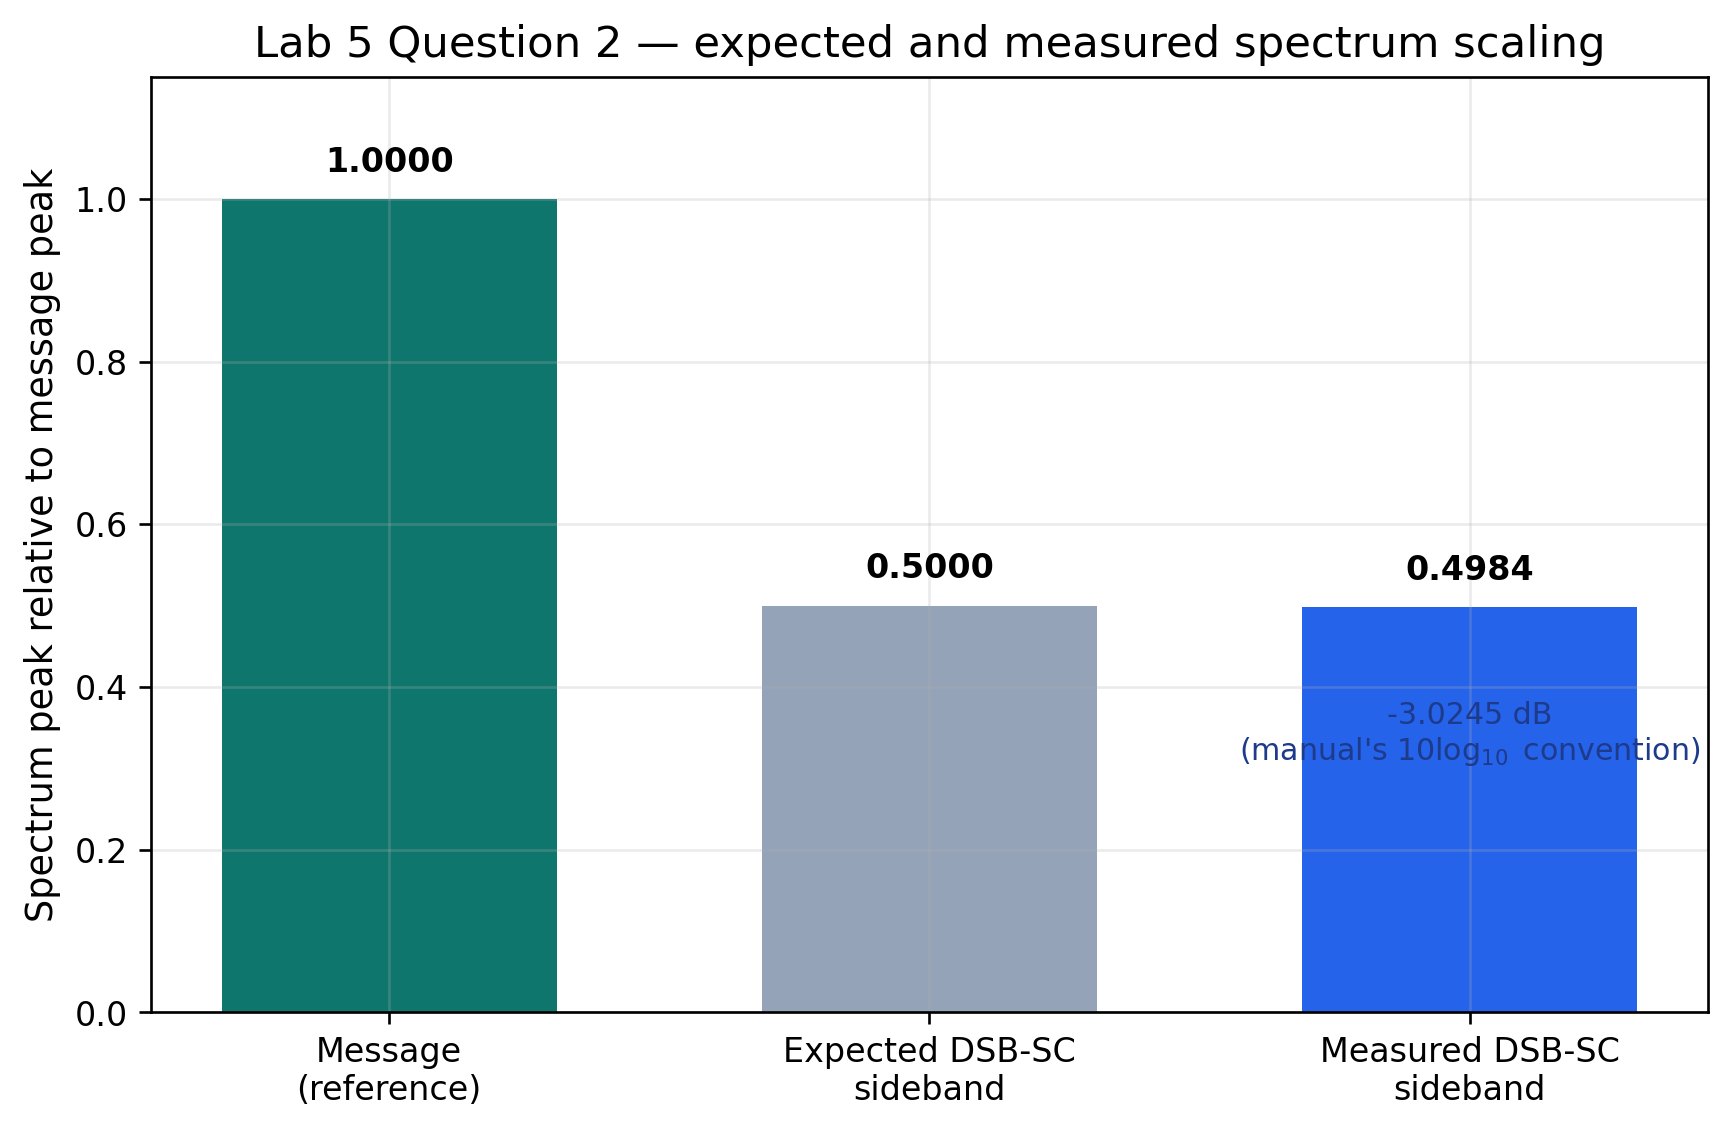
\includegraphics[width=0.88\textwidth]{lab5_q2_scaling.png}
  \caption{Later numerical verification of the Lab 5 Question 2 scaling. This graph supports the interpretation of the in-class spectrum screenshot; it is not presented as a class capture.}
  \label{fig:lab5-scaling}
\end{figure}
\weeklynote{\textbf{Attendance:} The full group attended both sessions.\\\textbf{What we did:} We rotated the computer role, worked through MATLAB and Simulink, and produced the final three-spectrum result.\\\textbf{Main difficulty:} Several possible plotting fixes were tried around one shared computer, and the exact decisive edit was not recorded.\\\textbf{Main lesson:} Preserve a known working baseline, change one thing at a time, and save the final script, model, scope capture and a one-line troubleshooting note.}
\section*{Document-wide unresolved details}
\begin{checkbox}
Before this becomes a final submission, complete the title-page group line, Lab 3 attendance/roles and weekly note, and later populate the deliberately blank Lab 1 and Lab 2 sections from primary class evidence.
\end{checkbox}
\end{document}
